\documentclass{article}

\usepackage{amssymb,amsmath,longtable, gensymb}

\usepackage[pdftex]{graphicx}
\graphicspath{ {Images/} {Images/eLoss/} {Images/CoordSys/} {Images/TrackerPics/} {Images/Field/} {Images/TrackingFlow/}}

\usepackage[margin=1in]{geometry}

\usepackage{hyperref}
\hypersetup{
    colorlinks=true,
    linkcolor=red,
    urlcolor=blue,
    citecolor=blue
}

\usepackage[backend=biber,sorting=none]{biblatex}
\addbibresource{mybib.bib}



\begin{document}

\title{Geane Track Fitting}
\author{Nicholas Kinnaird}
\date{\today}
\maketitle

% \renewcommand{\abstractname}{Assigned Problem}
\begin{abstract}

    In this document I will detail the concepts and mathematics of GEANE track fitting, as well as it's implementation in the gm2 simulation framework for the Muon g-2 Experiment at Fermilab. I will also detail the pecularities and intricacies of the code. This is done both for documentation purposes as well as a precursor to sections of my future thesis. This document assumes some familiarity with art on part of the reader, though such knowledge is not necessary for many sections. Note that the tracking code and framework is in constant development, so the details contained here within may be outdated at time of reading. 

\end{abstract}



\section{Introduction}

  The Muon g-2 Experiment at Fermilab will use tracking detectors in order to measure positron trajectories for the purpose of determining the beam distribution and its characteristics, both for the final $\omega_{a}$ result and for general beam diagnostics. A fraction of positrons originating from decaying muons will pass through the trackers. By fitting these tracks and extrapolating back to the average decay point, the beam can be characerized in a non-destructive fashion. The tracking can be done independently from the calorimeters in order to cross-check, or combined with them in order to provide the muon distribution that the calorimeters see for the direct $\omega_{a}$ calculation. It is arguable that this is the most important duty of the trackers. (Note that the integration of the two detector systems in the code has not been initiated.) It is also worth noting that there is a large percentage of tracks that hit the calorimeters hit zero or a small number of tracking modules, which this fitting code is not capable of handling.

  Each tracker module consists of 4 layers of 32 straws with a stereo angle of 7.5 degrees, the first two ``U'' layers oriented with the tops of the straws at a greater radial position, and the second two ``V'' layers oriented with the bottoms of the straws at a greater radial position. A tracking module is shown in Figure \ref{fig:tracker}. There are 3 tracker stations located at the 0, 12th, and 18th sections of the ring, counting clockwise from the top most point of the ring where the inflector resides. (Station 18 has been installed at time of writing, with station 0 planned for the fall. Station 12 is slated for the future sometime.) Each station consists of 8 tracking modules arranged in a staircase pattern that follows the curvature of the ring as seen in Figure \ref{fig:staircase}. Further hardware and electronics information regarding the trackers will be omitted in this document.

\begin{figure}[]
\caption{Shown is a picture of one of the many tracking modules used in the Muon g-2 experiment. The first layer of straws with a stereo angle of 7.5 degrees can be seen, with the other 3 straw layers hiding behind it. The beam direction is roughly into the page in this picture, and this view is what the decay positrons will see. Picture provided by James.}
\centering
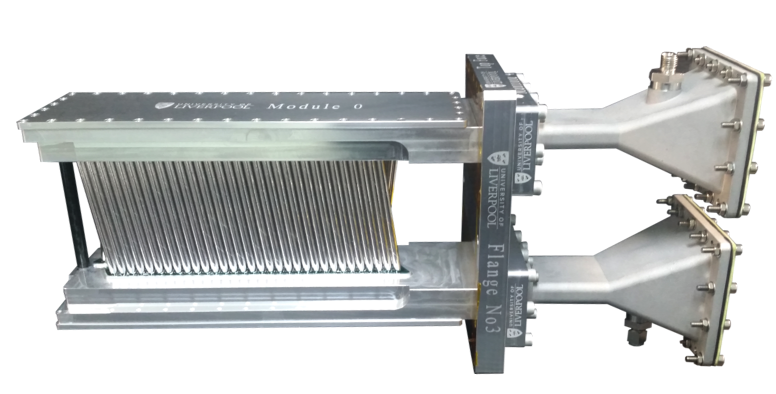
\includegraphics[width=0.9\textwidth]{Tracker}
\label{fig:tracker}
\end{figure}

\begin{figure}[]
\caption{Tracker modules are arranged in the shown staircase pattern. In green and dark blue is the edge of the vacuum chamber (where the dark blue identifies the modification that was made to the old vacuum chambers), and it can be seen that vacuum chamber walls lie at the ends of the outside tracking modules. The position of a calorimeter can be seen in teal at the right. The dark red spots are the locations of the pole tips.}
\centering
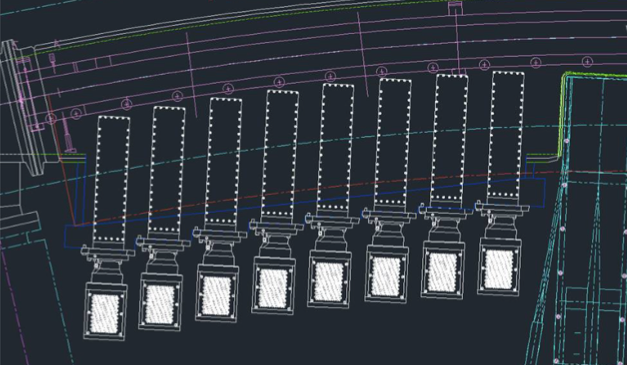
\includegraphics[width=0.9\textwidth]{trackerStation}
\label{fig:staircase}
\end{figure}


  Because of the proximity of the trackers to the muon beam, they will lie within a region of varying field. The radial field of the trackers rises from 0 Tesla at the outer ends to roughly .3 Tesla at the inner top and bottom ends, and the vertical field drops approximately 50\% from the storage dipole field of 1.451 Tesla. Shown in Figures \ref{fig:operaBy} and \ref{fig:operaBx} is the location of the tracker with respect to the horizontal and vertical fields respectively. If one thing can be said to be special to g-2 when it comes to tracking it is these large field gradients over the tracking detector region and several meter long extrapolation distance back to the muon decay point. This is one of the main motivations for using the Geane (Geometry and Error Propagation) fitting algorithm and routines, which has direct access to the field. 


\begin{figure}[]
\caption{Shown is the vertical field of the g-2 magnet in and around the storage region as calculated in Opera 2D. The center of the storage region lies at 7.112 m along the x axis. The black box shows the rough location of the tracker with respect to the field (size exaggerated slightly). It can be seen that there is a large inhomogeneity within the tracker space, goring from left to right.}
\centering
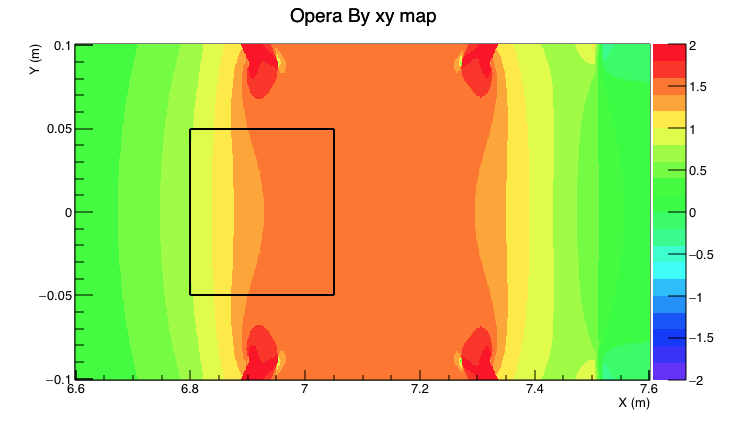
\includegraphics[width=0.9\textwidth]{operaBy}
\label{fig:operaBy}
\end{figure}

\begin{figure}[]
\caption{Shown is the radial field of the g-2 magnet in and around the storage region as calculated in Opera 2D. The center of the storage region lies at 7.112 m along the x axis. The black box shows the rough location of the tracker with respect to the field (size exaggerated slightly). It can be seen that there is a large homogeneity at the inner upper and lower ends compared to the right center. The shape of the pole pieces and tips can readily be seen.}
\centering
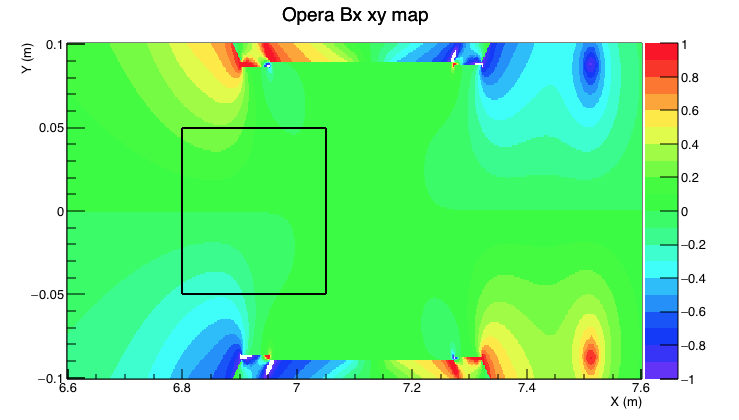
\includegraphics[width=0.9\textwidth]{operaBx}
\label{fig:operaBx}
\end{figure}

  The Geane fitting routines originated in Fortran with the EMC collaboration, and was used in the precursor E821 experiment as well as the PANDA experiment with some success. (cite stuff here?) (There might be some other instances of its use as well.) The core error propagation routines were at some point added to Geant4 under the error\_propagation directory which is included in all default installs. The tracking code strengths lie with its direct implementation and access to the Geant4 geometry and field, and its ability to handle the field inhomogeneties. The Geane algorithm code which makes use of the Geant4 error\_propagation routines follows the structure of \cite{geanemanual} and is detailed in the Formalism section in this paper. It is a relatively straight forward least squares global $\chi^{2}$ minimization algorithm. 



\section{Formalism}
\label{sec:Formalism}

    I recommend reading \cite{geanemanual}, Chapter 4 of \cite{Lavezzi}, and \cite{trajfit} in order to best understand the fitting algorithm. However, due to the at times confusing notation, ommitted equations or concepts, and differences between papers, I have attempted to summarize here the different sources and present the material in a more understandable and readable format. The implementation of the fitting algorithm into the code follows this section.

    One can define a $\chi^{2}$ for a track in the usual way by dividing the residuals of measured and predicted track parameters by their errors:
        \begin{align} \label{eq:chi2}
            \chi^2 = (\vec{p}-\vec{x})^{T} (\sigma^{-1}) (\vec{p}-\vec{x}),
        \end{align}
    where $\vec{p}$ are predicted track parameters from a fit to the measured track parameters $\vec{x}$, and $\sigma$ is a covariance matrix of errors on the fitted parameters. The Geant4 error propagation routines can be used to determine these predicted parameters and error matrices by propagating track parameters from some initial guesses. By minimizing this $\chi^{2}$ with respect to the track parameters one can then fit and improve the track. The Geant4 error propagation routines propagate particles along their average trajectories neglecting the effects of discrete processes, using a helix equation along small enough steps where the change in the magnetic field is small. The predicted parameters are then a function of path length: 
        \begin{align} \label{eq:pp}
            p_{l} = F_{l,l_{0}}(p_{0}),
        \end{align}
    where the path length can be defined how one wishes. In our system we have tracker planes defined at X positions, and limit path lengths to reach those planes. (From here on the dependence on path length or X position will be neglected, in favor of using plane indices.) In tandem, error matrices describing the expected distribution in true parameters about those predicted parameters due to said discrete process are also calculated:
        \begin{align} \label{eq:sigma}
            \sigma^{ij} = <p^{i}p^{j}> - <p^{i}> \cdot <p^{j}>,
        \end{align} 
    where i and j are track parameter indices. These parameter vectors are 5x1 objects defined in some track representation, as described in the \hyperref[sec:Coord]{Coordinate Systems} section. The propagation of these parameters and error matrices are done using transport matrices, which express the infinitesimal changes in parameters at some plane (or path length) with respect to the parameters at some previous plane (or previous path length):
        \begin{align} \label{eq:transport}
            \delta p_{N} = T_{N,N-1} \delta p_{N-1}, \\
            \sigma_{N} = T_{N,N-1} \sigma_{N-1} T_{N,N-1}^{T}.
        \end{align}
    Said transport and error matrices are 5x5 objects since the parameter vectors are 5x1 objects as described above. The calculation of these transport matrices, as well as details on the functional form of \ref{eq:pp} are shown in \cite{jacob}.

    With parameters defined on such planes, one can define the $\chi^{2}$ as: 
        \begin{align} \label{eq:chi2sum}
            \chi^2 = \sum_{i=1}^{N} [(p_{i}(p)-x_{i})^{T} (\sigma_{i}^{-1}) (p_{i}(p)-x_{i})],
        \end{align}
    where $p_{i}$ are the average predicted parameters from some general starting parameters $p$. At first order one can solely include the measurement errors on parameters, which fill in the diagonals of $\sigma_{i}$, if random processes can be neglected. Unmeasured parameters should have measurement errors of infinity (or some large value) along the diagonals in the code, which account for the fact that residuals for unmeasured parameters do not exist. When the error matrix is inverted all rows and columns of the matrix with these large numbers will fall to 0 in the $\chi^{2}$. 

    In order to get the best fit track, the $\chi^{2}$ should be minimized with respect to the initial track parameters p, and evaluated at some chosen or fitted parameters:
        \begin{align} \label{eq:minimize}
            \frac{\partial \chi^{2}}{\partial p}|_{p=p'_{0}} = 0,
        \end{align}
    resulting in
        \begin{equation}
        \begin{aligned}
            0 = \sum_{i=1}^{N}[ (\frac{\partial p_{i}(p)}{\partial p}|_{p=p'_{0}})^{T} (\sigma_{i}^{-1}) (p_{i}(p'_{0})-x_{i}) \\ 
            + (p_{i}(p'_{0})-x_{i})^{T} \frac{\partial(\sigma_{i}^{-1})}{\partial p}|_{p=p'_{0}} (p_{i}(p'_{0})-x_{i}) \\ 
            +  (p_{i}(p'_{0})-x_{i})^{T} (\sigma_{i}^{-1}) (\frac{\partial p_{i}(p)}{\partial p}|_{p=p'_{0}})]
        \end{aligned}
        \end{equation}
    where the 1st and 3rd terms are identical, and the 2nd term is small if one assumes that the error matrix doesn't change much with respect to the starting parameters. (Fair since most of the error comes from measurement, and as long as the initial guess is decent enough such that the path length through material doesn't change appreciably from one iteration to the next.) This simplifies to: 
        \begin{align} \label{eq:solve}
            \sum_{i=1}^{N} T^{T}_{i0} (\sigma_{i}^{-1}) (p_{i}(p'_{0})-x_{i}) = 0,
        \end{align}
    which is just the top term with 
        \begin{align} \label{eq:transport2}
             T_{i0} = \frac{\partial p_{i}(p)}{\partial p}.
        \end{align}
    To solve this make the substitution 
        \begin{align} \label{eq:psub}
            p_{i}(p'_{0}) = p_{i}(p_{0}) + \frac{\partial p_{i}(p_{0})}{\partial p} \Delta p_{0} = p_{i}(p_{0}) + T_{i0} \Delta p_{0},
        \end{align}
    where $p'_{0}$ are the improved starting parameters for the next iteration calculated from the previous starting parameters $p_{0}$, and $\Delta p_{0}$ are the changes in the starting parameters to improve the track. This equation can be plugged into the above if one makes the assumption that $T_{i0}$ does not change much from one iteration the next, which follows from the inherent nature of making small adjustments to the track in order to improve it.

    After simplifying one arrives at 
        \begin{align} \label{eq:deltap}
            \Delta p_{0} = \sigma_{p_{0}} \sum_{i=1}^{N} T^{T}_{i0}(\sigma_{i}^{-1})(x_{i} - p_{i}(p_{0})),
        \end{align}
    where
        \begin{align} \label{eq:cov}
            \sigma_{p_{0}} = [\sum_{i=1}^{N} T^{T}_{i0} (\sigma_{i}^{-1}) T_{i0} ]^{-1},
        \end{align}
    is the 5x5 covariance matrix of fitted parameters on the starting plane, whose diagonals describe the errors in the 5 track parameters on that plane and in the region close to it. (The fit does not directly return fit errors for track parameters on other planes.) $\Delta p_{0}$ along with $\chi^2$ is exactly what we want to determine since that is what allows us to fit and improve the track from iteration to iteration.

    However, since random processes should not be neglected for optimal tracking results, it makes more sense to return to the original $\chi^2$ in equation \ref{eq:chi2}, only now the included matrix and vector objects are combined into one large linear algebra equation. Instead of a sum over N 5x1 objects multiplying 5x5 error matrices, the vectors are combined into a single 5Nx1 vector multiplying a single 5Nx5N matrix. The 5x5 diagonal blocks of this large error matrix should now include the effects due to material processes as calculated in Geant from equation \ref{eq:sigma} as well as the measurement errors. 

    Because now parameters at one plane are no longer independent of the parameters at other planes, due to correlations from these random processes, it's necessary to add off-diagonal elements into the large error matrix. These 5x5 blocks come from 
        \begin{align} \label{eq:corr}
            \sigma_{MN} = T_{MN} \sigma_{N}, 
        \end{align}
    for the top diagonals, and the transpose for the bottom diagaonals, where M and N are two separate planes within the detector. ($\sigma_{N}$ is the error matrix on plane N calculated from the starting plane.) This follows from equation \ref{eq:sigma} evaluated at plane M with respect to a path length from plane N, and not plane 0, which is equivalent to \ref{eq:corr}. 

    You can then minimize the $\chi^{2}$ in the same way, only again with the matrix objects being aggregates of the per plane objects:
        \begin{align} \label{eq:deltafull}
            \Delta \vec{p}_{0} = \sigma_{p_{0}} \tau^{T}\sigma^{-1}(\vec{x}-\vec{p}),
        \end{align}
        %
        \begin{align} \label{eq:covfull}
            \sigma_{p_{0}} = [\tau^{T} \sigma^{-1} \tau ]^{-1},
        \end{align}
    where $\tau$ is the combined transport matrices from the individual 5x5 matrices, a 5Nx5 object.

    The unmeasured parameter errors of infinity still come into play in the final calculation in the same was as before. Because however these matrix objects are very large, and the tracking must have a certain amount of speed in order to keep up with data, it is useful to reduce the size of these matrices. (It also makes things easier programming wise. Note that there are other some other ways to speed things up, specifically the banded inversion method as described in reference \cite{trajfit}. This method was not used in favor of getting the code working in the simpler form in the first place, but it is a possiblity in the future to use this technique to speed things up even more.) It suffices to simply remove all rows and columns where said infinity values exist in the error matrix. This is mathematically equivalent to inverting the error matrix with the infinities included, which make all rows and columns where they exist go to zero. The associated unmeasured parameter rows in the residual vector and transport matrices must similarly be removed. This results in an Nx1 residual vector, NxN error matrix, 5xN combined transport matrix transpose, which multiply against the 5x5 covariance matrix out front to still result in a 5x1 fix to the starting parameters, and a scalar $\chi^2$ value. (Note that these element removals should be done just before the final calculation, and not higher up in the algrebra, otherwise plane correlations are not properly calculated.)

    By calculating the last two equations one can fit the track, acquire a $\chi^{2}$ describing the degree of the fit, determine how the track parameters can be improved at the starting point, and calculate errors on those starting parameters. This algorithm can be iterated a number of times to get a best fit track until successive iterations produce no improvement, where usually 3 or 4 iterations is enough. Note that there is remarkable robustness with respect to the initial starting parameters in fitting the track. Of course if the initial starting paramaters are too poor, then the fit will not converge. All of these calculations are completed within the \hyperref[sec:GeaneFitter]{GeaneFitter.cc} file within the framework.
 % Math stuff


\section{In the gm2 Framework}

  At the time of writing, the user should check out the artg4, gm2dataproducts, gm2geom, gm2ringsim, gm2tracker, and gm2utils packages of the gm2 repository, and be on the feature/trackDevelop branch in all instances. Every so often these branches are merged with the main develop branches, where the tracking code will work but might not have the latest code changes. In the future when the track reconstruction code is in a more final state, I imagine that the main g-2 analyses will all be based on particular versions of the develop branches.

  \subsection{Event Generation, Geometry, and Material}

    While not a direct part of the reconstruction and fitting code, there is relevant information with respect to event generation in the simulation upon which the reconstruction acts. Event generation before fitting is done using the mdc fcl files in gm2ringsim using the main simulation, where one should also include the tracker dummy plane geometry for truth comparison with the Geane fitting. These are built in the TrackerDummyPlane\_service and associated geometry files. At time of writing there are some modified mdc\#-geane fcl files which can readily be used. Only the necessary straw geometry and associated mother volumes, as well as the parallel world dummy planes are necessary to fit tracks, though including other geometry can of course change particle behaviour. All 3 main trackers are included in their original positions.

    Fcl parameters exist for the StrawTrackerCadMesh\_service and Straws\_service in order to turn material on or off at will, ``materialTracker'' and ``strawMaterial'' respectively. The rest of the geometry has to be manually changed and rebuilt in order to remove material if one wishes. These include VacuumChamberCadMesh and the World, as well as the ``buildSupportPost'' option in strawtracker.fcl, ``buildTrolly'' in vac.fcl (where the associated material is hardcoded in), and ``trolleySupportMaterial,'' also in vac.fcl. One should make sure to perform reconstruction with the same material parameters as were used in the event generation for proper results. (These options are primarily for debugging the tracking. Close to perfect results have been shown for tracking within a vacuum world, \href{http://gm2-docdb.fnal.gov:8080/cgi-bin/ShowDocument?docid=4876}{DocDB 4876} and \href{http://gm2-docdb.fnal.gov:8080/cgi-bin/ShowDocument?docid=4894}{DocDB 4894}.)


    \subsection{Reconstruction Flow}

    The overall tracking infrastructure and reconstruction flow can be seen in Figure \ref{fig:Infrastructure}. Data coming from simulation or the real experiment, are turned into art objects upon which the gm2 framework acts, and are grouped based on their positions in space and time. The RunGeane.fcl file (detailed more below) performs the entire chain within the blue box in Figure \ref{fig:Infrastructure}, excepting the track extrapolation stage. Within the reconstruction flow objects called Track Candidates are produced, which are the input to the Geane fitting code. The Geane fitting specific flow can be seen in Figure \ref{fig:GeaneFlow}. 


\begin{figure}[]
\caption{Shown is the infrastructure flow for the entire track reconstruction chain. In the green blocks are the sources of track data to fit, either from Geant simulation, or real data. In blue is the offline reconstruction block. Straw digits are formed in the digitalization step, those are then calibrated and grouped into time islands, clusters, and seeds which then combine to form track candidates. It is these track candidates which are the input into the Geane fitting code (and other future fitting code). The fitting code then outputs tracks which the track extrapolation stage will run over. This picture is taken from one of Tammy's talks. Note that there is some iteration here that is not shown.}
\centering
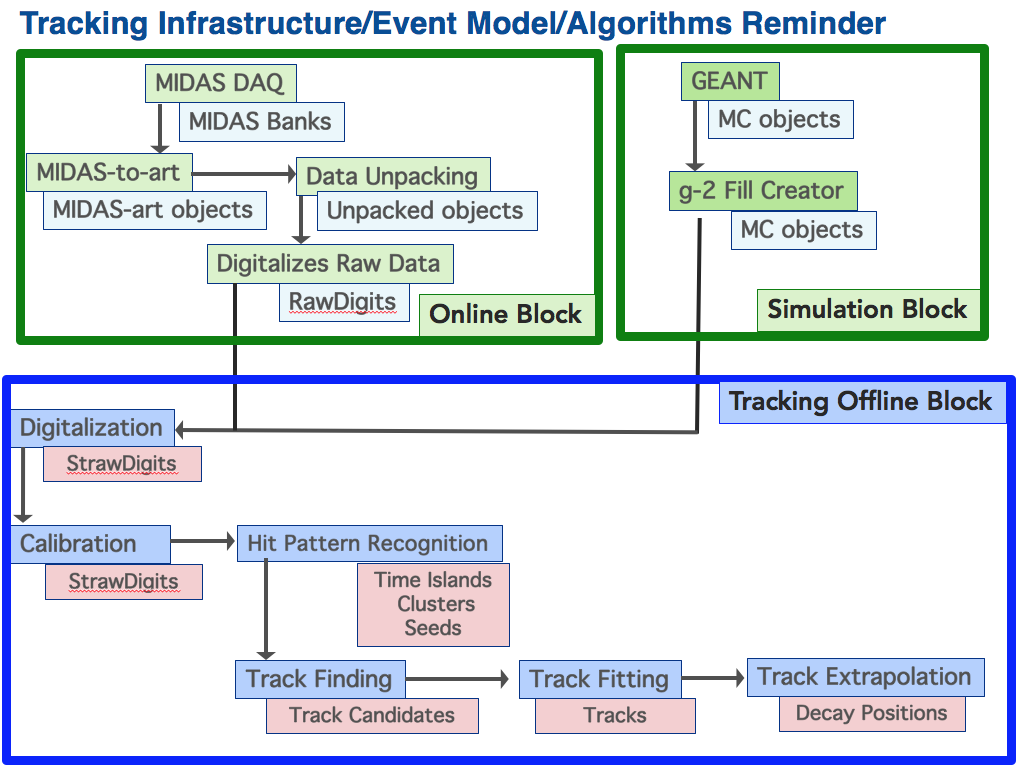
\includegraphics[width=0.9\textwidth]{TrackInfrastructure}
\label{fig:Infrastructure}
\end{figure}

\begin{figure}[]
\caption{Shown is the Geane fitting code flow. See the text for a thorough explanation of this flow, and the specifics of each box.}
\centering
\hspace{15mm}
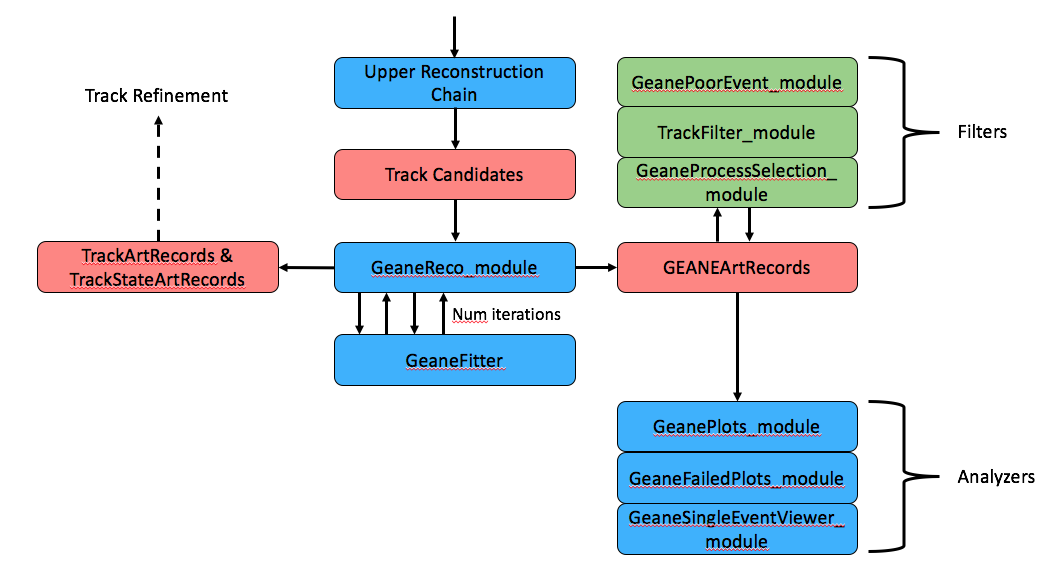
\includegraphics[width=0.9\textwidth]{GeaneFlow}
\label{fig:GeaneFlow}
\end{figure}


    The primary code for the Geane fitting are the GeaneReco\_module.cc and GeaneFitter.cc files. Detailed information regarding all of these files is given below, but here is provided a shorter summary. Track candidates drop into the GeaneReco file which initially sets up both the Geant4 world and the error\_propagation routines (once for all events), creates a GEANEArtRecord, and fills relevant track fitting objects. GeaneReco then tracks particles along their average trajectories in the Geant4 world, producing the matrix objects necessary for fitting as described in the Formalism section. All of these objects are stored within the GEANEArtRecord, which is then passed to the GeaneFitter class, which contains the methods and math needed for fitting the track again described in the Formalism section, after which a fit to the track is provided along with higher level track objects. GeaneFitter also provides an improvement to the track. GeaneReco and GeaneFitter then loop until the track fitting either succeeds or fails based on some metric, after which GeaneReco produces TrackArtRecords and TrackStateArtRecords, as well as a final updated GEANEArtRecord for the track. (Note that after a single iteration, one pass through GeaneReco and one pass through GeaneFitter, a $\chi^{2}$ and a fix for the track will be produced, but the track predicted parameters and objects will be based on the starting position and momentum guess before it has been updated, and so do not correspond to the fitted track. It's necessary to perform at least a second iteration for this reason, and is why no track converges under the strict criteria in under 3 iterations.) These TrackArtRecords can then pass to the extrapolation stage or go into some refinement stage (which has not been developed yet). The produced GEANEArtRecords can then be passed through filters and analyzers depending on what the user is investigating or looking at (again detailed below).


  \subsection{fcl File Specifics - RunGeane.fcl} 

    Again, reconstruction is performed using RunGeane.fcl in gm2tracker on the events generated from somewhere higher in the chain. It is important to explain some fcl parameters necessary for the reconstruction. First, there is a fcl parameter ``useSD'' for the Straws geometry service to turn off the straw sensitive detectors so that in the reconstruction phase hits are not regenerated. If this is not included, it will default to true and cause crashes in the reconstruction. Secondly, the RunGeane.fcl file loads all 3 trackers necessary for symbol and name definitions, but such that tracker 0 (or 18) is rotated such that the tracking planes are parallel to the global geant X axis (using the rotateArcTracker fcl parameter for the Arc service). This is done to avoid the issue of error propagation instability close to the Z axis, as detailed in \href{http://gm2-docdb.fnal.gov:8080/cgi-bin/ShowDocument?docid=4567}{DocDB 4567}, while at the same time still observing the correct azimuthally symmetric 2D field for the tracks. Track hits are rotated from their separate tracker frames to this one reconstruction frame with the GeaneWorldTracker[0], GeaneWorldTracker[12], and GeaneWorldTracker[18] transforms defined at the bottom of StrawTrackerCadMesh\_service.cc, and as detailed in the Coordinate Systems section. (In the future, if fields or geometries are not identical between trackers, the details here will have to be improved after changes have been made.) As a reminder there are material fcl parameters for the straws and straw trackers which should be the same as were used in the event generation. The RunGeane.fcl file also includes some analyzer and filter modules by default, which are detailed further below, and can be turned on and off at will.

    While the pieces of the chain before the track fitting (digitalizing, seeding, clustering, t0 finder, and track finding) are distinct and separate from the material detailed in this document, it is important to understand at some level those stages and the different options which will affect the tracking results. See a collaboration talk by Tammy, \href{http://gm2-docdb.fnal.gov:8080/cgi-bin/ShowDocument?docid=5601}{DocDB 5601}, for a general overview on this. Here is a short summary, not all method or file calls are detailed. Most of these files and parameters should be left unchanged unless one is familiar with the subject matter. 

    \begin{enumerate}

          \item{\bf{Digitalizer\_module.cc}} \\
          This module creates StrawDigits which will ultimately be combined to form the Track Candidates that the fitting will act over. It is the variables in this art record that are updated and correspond to real data, which straw was hit, the time of the hit, and the dca of the hit. The StrawDigits also contain a pointer to a struct of Monte-Carlo truth data, StrawMCDigit, which can also be accessed for track information. The Digitalizer module has several fcl parameters to change things like the gas drift time, drift model, allowing recorded negative times, and some particle cuts. By default it uses a Gaussian drift model which is called when the Digitalizer calls the DriftTimeModels.cc file, where it will gaussian smear the hit time from the MC digit time. These fcl parameters are located in digitalizerParams.fcl. The smearedDriftTimeSeed parameter should be set to 0 if one wants random results from run to run, which is necessary for grid jobs. The drift time model can also be set to the Garfield version, which will produce more realistic measurement parameters. If this is used the drift time calculator in the DriftDistanceCal module should also be set to the Garfield version. These more realistic hit data result in reconstructed tracks that haven't been fully examined yet.

          \item{\bf{TimeIsland\_module.cc}} \\
          Groups the digits from the Digitalizer in time. Has some options for changing the time window width. fcl parameters are located in recoIslandParams.fcl. There is some major ongoing work in relation to this module for dealing with real data, where there is a much increased number of hits closer in time. The short summary here does not reflect the difficult and important task that this module has.

          \item{\bf{ClusterFormation\_module.cc}} \\
          Groups neighboring digits in the same view to form clusters. fcl parameters are located in recoClusterParams.fcl.

          \item{\bf{T0Finder\_module.cc}} \\
          Calculates a t0 for the track. Has an option for which model to use for calculating said t0. The default is using truthData if one is running the tracking over simulated hits. If one is looking at real data there are other options. It's important to note that the t0 for a track can be difficult to calculate, and the current goal is to combine information from the calorimeter to get this number. fcl parameters are located in recoT0FindingParams.fcl.

          \item{\bf{DriftDistanceCal\_module.cc}} \\
          Calculates the drift times and distances within the straws based on the calculated t0 from the previous module. Has options for different drift calculators and parameters, including a ``useTrueModuleT0'' parameter for using mc truth information. The drift time is calculated from the digit hit time (calculated in the Digitalizer) minus the module t0. If true t0 is not used, then the dca smearing will not be perfectly gaussian. fcl parameters are located in recoClusterParams.fcl.

          \item{\bf{SeedFormation\_module.cc}} \\
          Groups neighboring clusters in the same module to form seeds. There are two fcl parameters for this module. The first is ``reconstructPosition'' which will fill seed nodes which form the seed, and essentially correspond to indidual digits - but which contain some left-right (LR) ambiguity information important for track fitting. The second is ``useGeometryLR'' which uses the straw geometry information to make an initial guess at the left-right choices for doublets within the track. fcl parameters are located in recoSeedParams.fcl.

          \item{bf{Aside}}
          It's important to note that there is another iteration of the time island and clustering modules which are improved now that better drift times and distances have been calculated from the previous modules, using the same fcl paramters. This will almost certainly change in the future as the tracking code becomes more developed.

          \item{\bf{TrackFinding\_module.cc}} \\
          Groups time islands and digits based on their positions in space. There are two finders available for use, fcl parameter trackFinderName, the Simple Track Finder (SimpleTrackFindingUtils.cc) and the Long Track Finder (LongTrackFindingUtils.cc). The former just runs off the generated time islands, and is more applicable to truth monte carlo data. If you use this, then the second clustering module and seed formation module can be left out of the reconstruction chain. The latter, Long Track Finder, forms track candidates based on combining seeds and is the default used. It also has stricter fcl conditions, such as a default cut of 6 or more planes hit for the track. Both finders make use of the SimpleCircleFitter.cc class which fits a circle to the U and V digit positions to calculate a starting position and momentum guess for the track, which is currently necessary for the Geane fitting. The Long Track Finder also has a least squares minimizer which is unimportant for the Geane fitting. There is also some functionality to make multiple track candidates from the same digits, which will be more useful once real data is coming in. fcl parameters are located in recoFindingParams.fcl, which then also links to some other fcl files depending on the finder used.


    \end{enumerate}

  \subsection{geaneFitParams.fcl}

    Because the Geane track fitting is the subject of this document, it will go more into detail of the Geane fitter fcl parameters, located in the geaneFitParams.fcl file. Some of these parameters are very likely to change or disappear in the near future.

    \begin{enumerate}

      \item{\bf{module\_type}} \\
      The ordinary art producer parameter which tells art which cc file to run, this is always set to GeaneReco unless the filename changes.

      \item{\bf{G4EVERBOSE}} \\
      This parameter corresponds to the iverbose level present in the Geant4 error\_propagation files and can be manually set here, from 0 to 5. It is for the debugging of deeper level Geane fitting code. Note that unless Geant is compiled with the flag by the same name setting this verbose level will do nothing. Since currently we utilize our own slightly modified error\_propagation files copied into the artg4/gm2Geane directory, it would be possible to remove the dependencies on this Geant4 build flag. Since however this will slow down the tracking it is the current choice to leave them in. 

      \item{\bf{trackingVerbose}} \\
      Geant4 tracking verbose level, from 0 to 5. This is always available but should only be used for debugging.

      \item{\bf{matrixDebug}} \\
      This boolean paramater turns on and off the copious matrix debugging output, used for deep level debugging. Note that these outputs are included in the log file and the log file threshold needs to be set to ``DEBUG''. In the future it might be beneficial for speed reasons to remove completely these debugging outputs. This parameter should always be turned off if looking at a large number of events.

      \item{\bf{numPassesWireFit, numPassesMainFit}} \\
      These are parameters used for the Left-Right sequence checking routines for a full fit. numPassesWireFit is the number of passes that the track should be fit to the wire centers, before which the best sequences were passed to the main fit code which would iterate a number of times equal to numPassesMainFit. It was observed in the past that 2 or 3 passes for each of these was sufficient for good tracking results. 

      \item{\bf{convergenceCriteria}} \\
      This is a scalar convergence criteria telling whether the track fitting has been successful or not, with a default value of .1. As long as the current iteration $\chi^{2}$ minus the previous iteration $\chi^{2}$ is less than this value, the track is considered to have converged, otherwise it continues iterating until it succeeds, fails, or is manually cut off at a larger number of iterations, depending on the fit mode used.

      \item{\bf{useCircleGuess}} \\
      This boolean parameter tells the code whether to use the circle fitter results for the track starting guess or not, called in the track finding part of the chain. It's default should remain true unless one wants to return to the uniform starting parameter smearing for debugging purposes.

      \item{\bf{lockLowDCAs}} \\
      This is a temporary fcl parameter which will take measured hits with small values (currently hardcoded to 300 um) and change them to the wire center positions, at the same time locking the LR choices to the center. This will be necessary when fitting data due to the large measurement uncertainty of hits close to the wire, and at the same time speeds up the code with one less LR choice to iterate over.

      \item{\bf{fitMode}} \\
      This is the most important fcl parameter for the Geane fitting. It defines what type of fitting mode you'd like to use for fitting the incoming track candidates. There are currently 4 separate fitting modes. ``truthLRFit'' only works with simulated data and will fit to the unambiguous LR UV values from the digits. ``wireFit'' will fit a track to the wire centers of the incoming digits, with a corresponding uniform error equal to the gas diameter. ``mainFit'' will first do a wire fit to the track in order to make an initial guess at the LR choices for each hit, and will then fit to those LR choices. (At the time of writing this it actually does a second wire fit in the middle where it locks LR choices for doublets where the LR choice is guaranteed to be known.) Finally there is the ``fullSeqFit'' which will first do the wire fit, and will then go about checking all LR sequences before doing full fits on the set of best sequences. (This LR procedure is detailed lower in the code somewhere.)

      \item{\bf{rseed, yPosChange, zPosChange, xMomChange, yMomChange, zMomChange}} \\
      These are the uniform smearing bounds for the starting position and momentum of the track from truth, units of mm and MeV. These are largely unused now since the circle fitter provides a level of smearing automatically when it's used, but should be kept for future debugging purposes. The rseed parameter is the number seed for the random number generator. The default should be 0 for the root TRandoms unless one wants to reproduce results.

    \end{enumerate}


  \subsection{cc Files}

    Here will be given a summary of the different cc files used in the Geane track fitting as shown in Figure \ref{fig:GeaneFlow} and explained up above, as well as extensive detail where necessary. 


    \begin{enumerate}

      \item{\bf{GeaneReco\_module.cc}} \\
      This file consists of the main code which sets up the GEANE track fitting, pulls in upstream data products, interfaces with both Geant4 and the gm2 art framework, outputs TrackStateArtRecords and TrackArtRecords for use downstream, as well as GEANEArtRecords to analyze. 

      It's methods consists of:

        \begin{itemize}

          \item{produce} \\
          General overriden produce method. Calls main track fitting code on an event by event basis. Produces data products for downstream use.

          \item{InitializeGEANE} \\
          Geant4 GEANE (error\_propagation) initialization method called by the constructor, once per run.

          \item{trackFitting} \\ 
          Sets up variables and objects for track fitting after reading in upstream data products (track candidates and dummy planes). Contains calls to track fitting iteration loops. Also contains LR sequence checking routines.

          \item{modifyMeasuredParams} \\ 
          Short method for LR sequence checking, modifies measured parameters based on particular sequence.

          \item{fittingLoop} \\ 
          Method which contains the fitting loop code which successively calls errorPropagation in the same file and the GeaneFitter for fitting the track. The angleCorrection method is called each iteration to update the UV measured positions and errors depending on the track momentum. (Before it is called the errors are reset so that they are not double corrected.) There is also a method parameter for updating the LR choices based on the fit at each iteration, which is only used when doing a ``mainFit'', which improves the final tracking results. This method will loop inside itself until convergence is achieved or the max number of iterations is reached (or fitting fails).

          \item{checkExtraneousFailureModes} \\
          This is a short method used for checking if track results might be off because of other extraneous reasons.

          \item{errorPropagation} \\ 
          This method tracks particles through the detector using Geant4 error propagation routines with the correct geometry and field. It builds transport matrices, error matrices, and predicted parameters which are the objects used for fitting the track. It tracks on a plane by plane and step by step basis. These routines can be used to track particles forwards and backwards, where the forwards tracking is used in the code. Changing to backwards tracking would be very non-trivial. Add more detail here later..

          \item{angleCorrection} \\
          Method to iteratively correct measured parameters from a radial DCA value to a U or V value based on the momentum of the track and approximating a constant field within the straw. Also corrects the errors using a simple straight line approximation which is good enough. See appendix section for more details on how this works.


go into detail somewhere about what this method is doing and where??



        \end{itemize}

      \item{\bf{GeaneFitter.cc}} \\
      This file consists of the main track fitting chi2 algorithm. It multiplies measured parameters, predicted parameters, error matrices, and transport matrices together to produce a chi2 for the track and an improvement to the starting paramters. It also reads in the measured hits errors in order to properly fit the track. There is a fcl parameter matrixDebug which can be used to turn on or off the many large matrix cout debugging statements.

        \begin{itemize}

          \item{TrackCorrelation} \\
          The main matrix multiplication routines.

          \item{preSequenceChecking} \\
          A method in order to create a hybrid wire / U or V error matrix for L/R sequence checking. Only called once per event.

          \item{sequenceChecking} \\ 
          The main L/R sequence checking method for an individual event. This method is called many thousands of times as each U or V sequence is checked. Ignore for now.

          \item{convertTo} \\
          Some methods for converting Eigen 5 vectors from GeV cm to MeV mm and vice versa.

        \end{itemize}

      \item{\bf{GeanePlots\_module.cc}} \\
      The main analyzer/plotting module which runs on the output GEANEArtRecords produced upstream. This creates many plots including chi2 distributions, p value distributions, number of iterations, track parameter, residuals, pulls, etc. Truth information for these plots is currently necessary as written, but can be take out in the future for real data. There are some fcl paramters to make cuts on different parameters. There are also some other plotter modules which are similar but much reduced in scope. reference geanePlotsParams.fcl file here.

      \item{\bf{GEANESingleEventViewer\_module.cc}} \\
      include a plot or two of what the single event viewer can show, how to use it (specify events or not)

      \item{\bf{GEANEProcessSelection\_module.cc}} \\
      mention how this insn't fully devloped yet

      \item{\bf{GeaneFailedPlots\_module.cc}} \\
      explain failed plots mode, included plot

      \item{\bf{GeanePoorEvent\_module.cc}} \\
      selection on bad events and why

      \item{\bf{geane plots macro}} \\
      I think also include some notes about this guy

    \end{enumerate}


  \subsection{Other useful fcl files}

    There is a number of other fcl files which are currently included in gm2tracker which are useful for various analysis or fitting purposes. These are relatively simple and straight forward fcl files which can be deleted, combined, or changed however the user wishes depending on what they are looking at. They are typically used on produced sets of GEANEArtRecords.

    \begin{enumerate}

      \item{\bf{RefitGeane.fcl}} \\
      This file simply refits a previously produced set of track candidates, typically used for refitting failed or bad events from a previous attempt at fitting. One can make changes to the fitting code, refit, and compare to previous results.

      \item{\bf{makeGEANEPlots.fcl}} \\
      This file will call the main GeanePlots analyzer module for producing plots about the GEANEArtRecords, useful for when one wants to add or remove plots after tracks have already been produced.

      \item{\bf{ProcessSelectionGeane.fcl}} \\
      This file will call the filter on different physical processes that events have undergone within the tracker region, if one wishes to separate events based on this criteria.

      \item{\bf{makeGeaneSingleEvent.fcl}} \\
      This file will take produced GEANEArtRecords and call the single event analyzer on the specified set of events. This is useful for analyzing single events to see where rare errors crop up, if tracks are kinking, for debugging purposes, etc. This should not be used for a large number of events.

      \item{\bf{filterTracks.fcl}} \\
      This file will filter on whether art events successfully produced a GEANEArtRecord or not (succeeded or failed), which is useful for reducing the size of art files which contain many events that do not hit the tracker or don't hit enough planes.

      \item{\bf{fileMerge.fcl}} \\
      This very general file will simply combine the set of art files that are passed to it, useful for reducing the number of files one has to deal with.

    \end{enumerate}


\subsection{Code details}

Building and multipilying transport and SC2SD matrices
Converting things to eigen objects

JacobianToUV stuff - or combine with other coordinate transform stuff
Matrix accumulation/reduction
Notes on loop indices, start points and such



\subsection{Code peculiarities / notes}

Where to structure this in the file?

Notes on coordinate systems I use - UV pointing outward vs XYZ, XUV x being forward, UVW in geante src, maybe IJK/TUV in one paper-prob not, GeaneTrackerWorld[0,12,18], rotateArcTracker (bit more specific), magnetic field access coordinates?, JacobianToUV

accessing the field in a specific way



\section{gm2Geane package in artg4 - eloss, brems, ionizations, msc}

See many docdbs by Nick Kinnaird on geane updates for more info if wanted. Summary of stuff here.


  There is a folder under artg4/gm2Geane, where slightly (but importantly) modified geant/geane code that the geane track fitting uses is located. Most importantly is that the reconstruction was taking too much energy away from the particle during propagation due to bremsstrahlung, so that has been removed. (Thanks James for help with this.) (Probably explain flow of file - extrapolator tables etc.).

  Besides those associated files, all files from the geant folder ``error\_propagation'' have been copied into this directory as well, with the only non-name changes lying in gm2GeaneFreeTrajState.cc. (Many files had to be copied due to naming/linking - some could probably have been omitted but I decided to copy the whole folder.) Ionization and multiple scattering errors have been modified according to Lavezzi thesis (explain more) - with no improvement in results unfortunately. (Probably turn defaults back to original code (still gm2Geane) with the option to turn things on somehow if desired - at least leave them in for future tuning.)

Should I go more in depth about the error\_propagation/gm2Geane source code? Probably - at least for certain main files.


Add many plots and pictures of things - pulls, single events, tracks, etc etc.

\begin{figure}[]
\caption{Shown here is the energy loss between the first and last hit in the tracker from simulation. (Momentum magnitude difference.) Sources of energy loss come from ionization and bremsstrahlung processes, which account for the long Landau tail running off to infinity. The distribution has a mean of approximately 220 keV and and peak centered at about 150 keV, which is reasonable for the material composition of our trackers and tracker gas. More than 50\% of the energy loss comes from the mylar walls of the straws as seen in the simulation.}
\centering
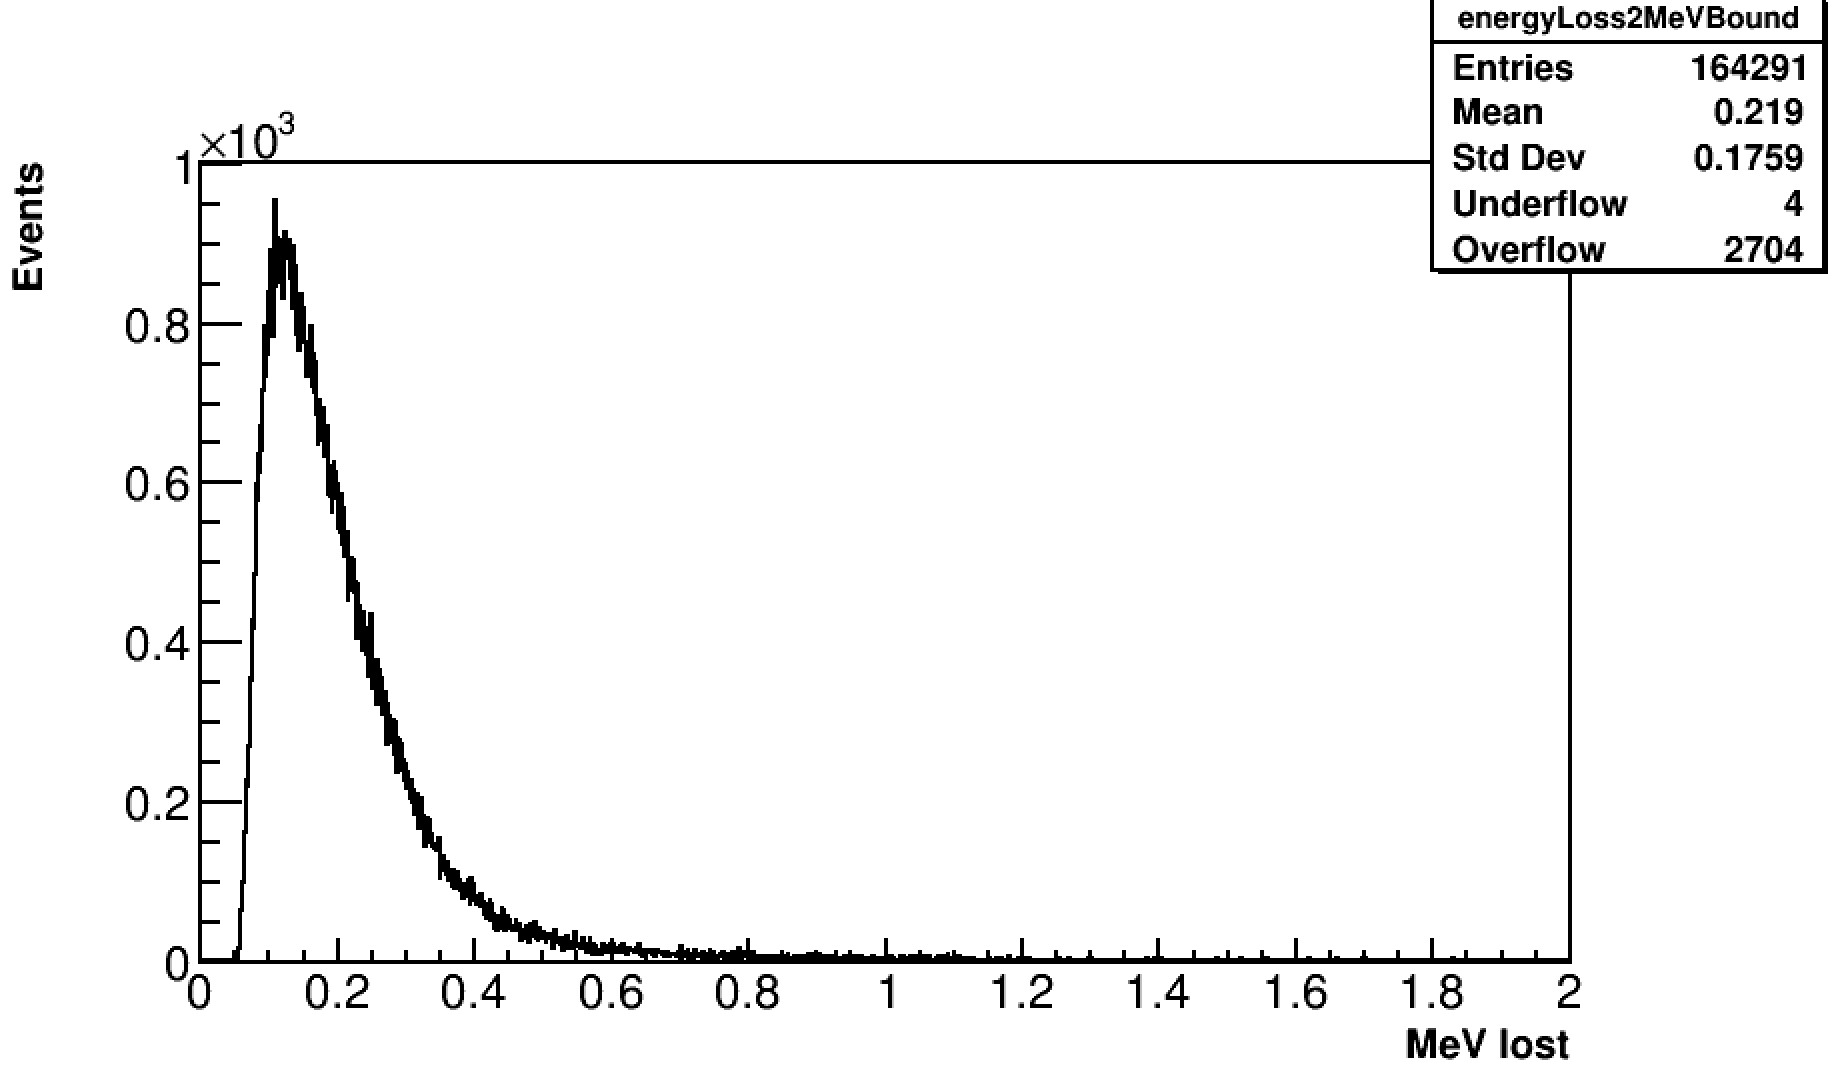
\includegraphics[width=1.0\textwidth]{eLoss}
\label{fig:eLoss}
\end{figure}

\begin{figure}[]
\caption{It was noticed during the course of debugging that the Geant4 error\_propagation routines were consistently removing too much energy on average from all tracks as they passed through the tracker during reconstruction. It was discovered that the Geant4 tables were taking out too much energy due to bremsstrahlung processes and it was decided to remove this effect. The left plot shows in a red the true particle momentum as a function of X distance through the tracker, and in black the reconstructed momentum before bremsstrahlung was taken out of the reconstruction for a single event. The differing slopes signify the problem. The right plot shows the same event but with bremsstrahlung taken out. Notice scale change, and that the reconstructed momentum aligns much more readily with the truth.}
\centering
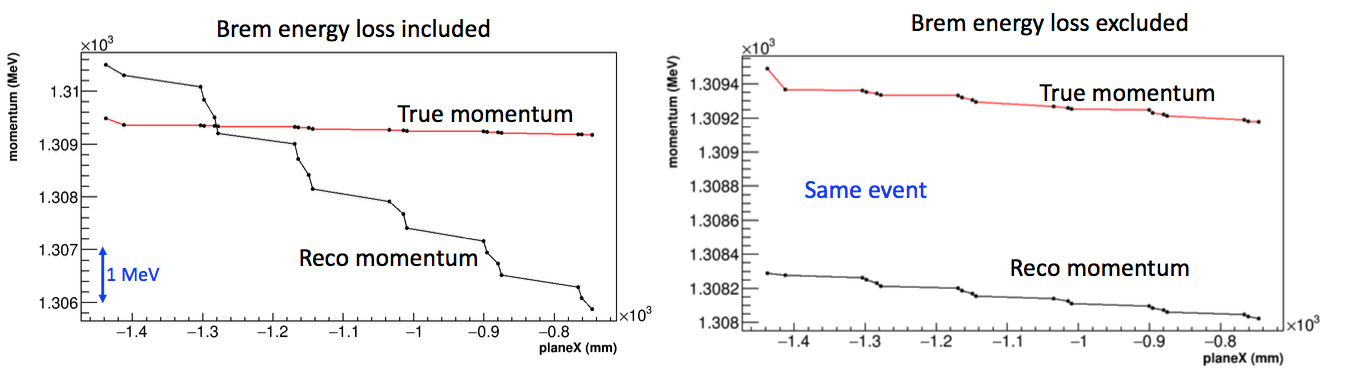
\includegraphics[width=1.0\textwidth]{bremComparison}
\label{fig:bremComparison}
\end{figure}


% /////////////////////////////////////////////////////////////////////////////////////
\section{Coordinate Systems}

  The only material not covered here in full detail is the mathematical explanation of reference frames, for which one should see the reference papers. It suffices to summarize as follows: GEANE objects (matrices and parameter vectors) are defined and calculated in the Geant4 source code in the free particle system. Then there is an intermediate surface system defined in XYZ, as the Geant4 surface trajectory system must be defined in an orthogonal coordinate system, before which parameter objects are converted to the most natural detector system of XUV. (Important note - be very careful with coordinate system variables, letters are reused between different papers and code bases with different configurations and meanings constantly.)


\begin{figure}[]
\caption{Shown here is a picture of the 3 trackers in the world geometry in their approximate positions. First note the world coordinate system shown in the bottom left of the plot, where the origin lives at the center of the ring. Tracks are then generated and read out from the trackers in their three world positions in red. Due to the reconstruction bug where tracks improperly reconstruct if their momenta is too aligned with the globabl Z axis, the reconstruction rotates the entire arc including tracker 0 to the blue position, where planes are parallel in X, and this problem is avoided. Track parameters from the 3 positions are then rotated to this reference frame by the amounts shown on the plots for the reconstruction stage, and at the end are rotated back.}
\centering
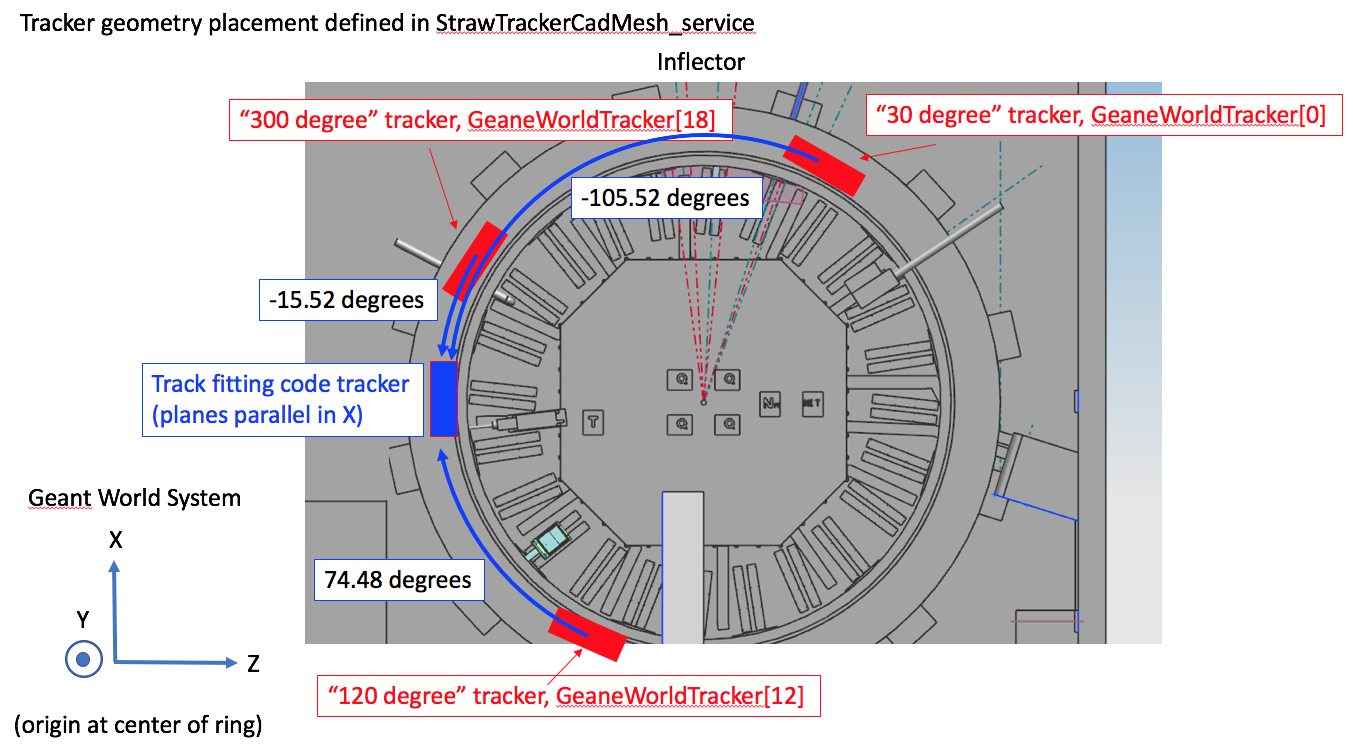
\includegraphics[width=1.0\textwidth]{WorldCoordSys}
\label{fig:WorldCoordSys}
\end{figure}

\begin{figure}[]
\caption{This picture shows the coordinate system in which the the Geane track reconstruction is performed, in relation to the world coordinate system. The origin remains at the center of the ring, with the tracking planes parallel in X in the reconstruction, going forward in number. Y is vertically up, and Z is horizontally to the right. U and V are defined such that they have greater values with higher radii and increasing straw number.}
\centering
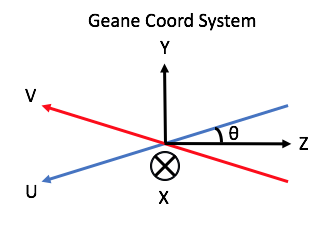
\includegraphics[width=0.6\textwidth]{GeaneCoordSys}
\label{fig:GeaneCoordSys}
\end{figure}


$1/p, \lambda, \phi, y_{\perp}, z_{\perp}$, free system

$1/p, py/px, pz/px, y, z$, surface system

$
\begin{pmatrix}
u \\
v \\
\end{pmatrix} =
\begin{pmatrix}
-\sin{\theta} & -\cos{\theta} \\
\sin{\theta} & -\cos{\theta} \\
\end{pmatrix}
\begin{pmatrix}
y \\
z \\
\end{pmatrix}
$, yz to uv matrix, where $\theta$ is $7.5\degree$, the 5x5 transformation is just a 1 in the top left corner, and then this matrix in the remaining 2 diagonal blocks

$1/p, pu/px, pv/px, u, v$, uv system

% /////////////////////////////////////////////////////////////////////////////////////




% it seems I have to cite the references in order for them to be added to the paper - some weird build issue, just do it here until I cite them naturally in the paper
\cite{jacob}, \cite{energyloss}

\printbibliography


\section{notes and other}

 Due to the CBO of the beam, 1 tracker accounts for ~90\% of the physics, and a second tracker accounts for much of the remaining. (Find/learn sources for this to explain a bit better..)

  starting error matrix

  linking equations to code variables

  initial errors into tracing/error propagation?

  mention that it's possible to make a Kalman filter which uses the geane matrix objects? and that I didn't do so because we wanted two separate methods for the tracking originally and someone else was working on the kalman filter? (and the chi2 minimization was used in the last experiment)

  make a subsection on the left-right ambiguity work 

  negative chi2 stuff

  note on older branches for development at all?

  \subsection{Kalman Filter}

    There is some precedent for using the error propagation matrix objects within a Kalman filter as detailed in the Lavezzi thesis \cite{Lavezzi}, but due to the circumstances following the creation of this code that technique was not followed. At the beginning of development, a Kalman filter was being started in tandem by others, which has since fallen by the wayside. In order to have two separate methods for fitting however, the least squares global minimization was chosen. The simpler method was also chosen as the author was unfamiliar with track fitting and coding in general when beginning development.



\section{Acknowledgements}

Should I put an acknowledments section in? (Rob, Rob, James, Joe)
From a technical document perspective maybe not?


\appendix
\section{Appendix}
\label{sec:Appendix}

  \subsection{Angular correction}

  Our straws don't actually measure U and V coordinates directly, but instead measure the distance of closest approach radii deriving from measured hit times. In order to utilize the minimization procedure on measured track parameters these radii must first be converted to U and V parameters, and similarly for the U and V errors. (Note that a future Kalman filter will not be subject to this disadvantage.) This is done in the calcMeasuredParams method at the bottom of the GeaneParamUtils class. These conversion corrections will be dependent on the angle of the track, so it's imporant to note that during each successive iteration, the ``measured'' parameters are adjusted by the latest ``predicted'' momenta. It was found that for the error correction, a simple straight line correction was sufficient for ideal results. For the position correction, it was found that a constant field correction for curved tracks was sufficient.

  To calculate these corrections, first the momentum perpendicular to the straw measurement axis can be ignored since it won't affect the U or V value. Because the positron tracks curve in only one direction through the tracker, one needs to calculate the correction depending on whether the track went to the left or right side of the wire. See Figure \ref{fig:angularCorrection} for a pictorial representation of the problem. The calculation of the right side correction follows, with the left side correction being calculated in a similar manner.

	\begin{figure}[]
	\caption{Shown here is a positron passing through a straw. The desire is to convert the measured parameter d into a U or V position, which can be done by approximating the particle trajectory as a circle in a constant magnetic field over the course of the straw and using trigonometry. Sizes and angles are exaggerated.}
	\centering
	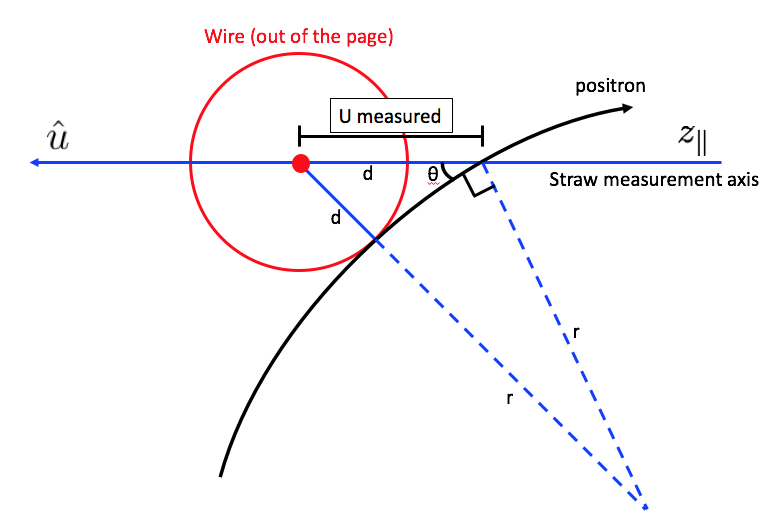
\includegraphics[width=1.0\textwidth]{angularCorrection}
	\label{fig:angularCorrection}
	\end{figure}

  To solve for the measured U (or V) value, we can use the equation:
	\begin{align}
		(r+d)^{2} = r^{2}+u^{2}-2ru\cos(90+\theta),
	\end{align}
  where the 90 degrees is approximate for large curvature of tracks. The angle $\theta$ can be determined from 
	\begin{align}
		\hat{z_{\parallel}} \cdot \hat{p_{\parallel}} = \cos{\theta}, \hspace{.1cm} \theta = \cos^{-1}{\frac{p_{\parallel}}{p}}, 
	\end{align}
  where $p_{\parallel}$ is the positron momentum parallel to the $z_{\parallel}$ axis at the wire plane and can be determined within the code. (The $z_{\parallel}$ axis simply stands for the axis perpendicular to the straw and parallel to the U measurement axis, but opposite in direction. At the end this calculated U value will simply be added or subtracted to the wire center U position depending on which side of the wire the positron travelled.) Using some trig identities and solving for u gives
	\begin{align}
		u = -r\sqrt{1-(\frac{p_{\parallel}}{p})^{2}} + \sqrt{d^{2} + 2dr + r^{2}(1-(\frac{p_{\parallel}}{p})^{2})},
	\end{align}
  for the right side correction, and 
	\begin{align}
		u = +r\sqrt{1-(\frac{p_{\parallel}}{p})^{2}} - \sqrt{d^{2} + 2dr + r^{2}(1-(\frac{p_{\parallel}}{p})^{2})},
	\end{align}
  for the left side correction. (Corrections to v are identical.) The radius of the particle circle can be calculated from the circular momentum and magnetic field at the predicted hit position. The straightline correction is done simply using the Pythagorean theorem in a simpler manner, with the correction to the errors then being
	\begin{align}
		\sigma_{uv}' = \frac{\sigma_{uv}}{\sqrt{1-(\frac{p_{\parallel}}{p})^{2}}}.
	\end{align}


\subsection{Matrix Transformation}
\label{sec:MatTransf}

  Transport matrices are accumulated as
      \begin{align} %\label{eq:nolabel}
        T_{mn} = T_{mk}T_{kn},
      \end{align}
  where the indices can stand for either plane numbers or step numbers, and converted by 
      \begin{align} %\label{eq:nolabel}
        T_{mn,s} = A_{m} T_{mn,f} A_{n}^{-1},
      \end{align}     
  where the indices s and f stand for the surface and free trajectory states respectively, and A is the Jacobian transformation from the free state to the surface state on a particular plane m or n. See \cite{jacob} for the calculation of these Jacobians. The error matrices in the surface state can be grabbed directly from the Geant code unlike the transport matrices, or if necessary can be converted as
      \begin{align} %\label{eq:nolabel}
        \sigma_{m,s} = A_{m} \sigma_{m,f} A_{m}^{-1}.
      \end{align}  



\subsection{GEANEArtRecord.hh} 
\begin{longtable}{|p{16cm}|}
% \scriptsize
\caption{GEANEArtRecord.hh active variables. This is subject to change. GEANEArtRecord contains vectors of variables on planes, as well as larger objects containing information about the whole track. Note that Eigen matrix objects cannot be stored into art data products. For this reason, and for minimal code changes, it was decided to add a data object for each Eigen member, made up of vectors with the word ``Data'' tagged at the end. The data objects are saved when creating GEANEArtRecords using a utils file. In analyzers accessing the GEANEArtRecords, these data objects are then swapped into the Eigen objects using the same utils file.}
 
\label{tab:artRecord}

% \begin{tabular}{|p{16cm}|}

  \\ \hline

enum GeaneHitSide \\ 
\textit{An enum for which side of the wire the track hit is guessed or calculated to have passed. Options are gLeft, gRight, gCenter, gNA\_side, and gUnknown. The first three are self explanatory, gNA\_side simply means there wasn't a hit, and gUnknown is used within the LR sequence checking part of the fitting code where any hits with said value or looped over to try and find the best choice.} 

  \\ \hline

art::Ptr \textless{} gm2strawtracker::TrackCandidateArtRecord \textgreater{} candidate \\
\textit{One track corresponding to one candidate corresponding to one GEANEArtRecord for the whole track.} \\ \hline

std::vector\textless{} art::Ptr\textless{} gm2truth::GhostDetectorArtRecord \textgreater{} \textgreater{} dummyPlaneHits \\
\textit{Associated dummy plane hits on planes aligned with straw wires, vector consists of hit dummy planes corresponding to hit wire planes (if a straw plane was skipped but that dummy plane was hit, it is not included in this vector. Vector has size N = num hits in straws that form the track +1 for the 0 plane.)} \\ \hline

int failureMode \\ 
\textit{Different failure modes for failed track reconstruction, 0 means it passed.} \\ \hline

double chi2 \\ 
\textit{Chi2 for whole track.} \\ \hline

std::vector\textless{}double\textgreater{} chi2Iterations \\
\textit{Chi2s for whole track for different iterations.} \\ \hline

std::vector\textless{}double\textgreater{} chi2Planes \\
\textit{Individual chi2s on each plane which add up to total chi2, vector consists of hit planes with size N.} \\ \hline

int numIterations \\
\textit{Number of iterations to converge.} \\ \hline

unsigned int dof \\
\textit{DoF of track = number of hit planes - 5 track parameters.} \\ \hline

double chi2DoF \\
\textit{chi2/dof} \\ \hline

double pValue \\
\textit{Fit pValue for whole track.} \\ \hline

double energyDiff \\
\textit{energy loss between first and last hit in track - from truth, for material characterizing} \\ \hline

std::vector\textless{}double\textgreater{} startingTrackParameters \\
\textit{Starting parameters for track: size 6, 3 position then 3 momentum, x y z px py pz, best starting parameters updated after each iteration, starting parameters x position defined before first hit.} \\ \hline

std::vector\textless{}double\textgreater{} startingTrackGuessOffsets \\
\textit{Size 10, x y z px py pz p 1/p pu/px pv/px offsets in different starting track parameters for plotting purposes.} \\ \hline

int trackNumPlanesHit \\ 
\textit{Total number of planes hit.} \\ \hline

int trackFirstPlaneHit \\ \hline

int trackLastPlaneHit \\ \hline

std::vector\textless{}int\textgreater{} trackPlanesHitList \\
\textit{List of hit planes, with missed planes excluded from the vector. Ex. 1 2 4 5 8 9} \\ \hline


std::vector\textless{}std::vector\textless{}double\textgreater{} \textgreater{} wireUVPositions \\
\textit{Wire center U and V postions, first vector is track param vector size 5 (0 1 2 unfilled, 3 is U, 4 is V), second vector is planenumber from 0 - 32  (formatted this way to align with other similar vectors - can probably be reduced.)} \\ \hline

std::vector\textless{}double\textgreater{} measuredDCAs \\
\textit{Vector of measured DCAs for hit planes, with size 33. Mainly to hold on to smearing values for now.} \\ \hline

std::vector\textless{}double\textgreater{} UVerrors \\
\textit{Vector of UV measurement errors for planes 0-32. Built in order to accomadate varying errors in the future.} \\ \hline

std::vector\textless{}double\textgreater{} planeXPositions \\
\textit{Vector of X postions of hit wire planes with size 33 (0 - 32), 0 plane being in front of the first module that was hit.} \\ \hline

std::vector\textless{}std::vector\textless{}double\textgreater{} \textgreater{} geaneMeasuredParameters \\
\textit{Measured GEANE parameters, first vector is param num 0 - 4, second vector is plane number 0 - 32, units are MeV mm. 1/P, Pu/Pz, Pv/Pz, U, V - only U or V is filled at the start of the GEANE fitting module.} \\ \hline

std::vector\textless{}std::vector\textless{}double\textgreater{} \textgreater{} geanePredictedParameters \\ 
\textit{Predicted GEANE parameters, first vector is param num 0 - 4, second vector is plane number 0 - 32, units are MeV mm. 1/P, Py/Px, Pz/Px, Y, Z - all params filled in tracing stage of GEANE fitting module - coord system has to be orthogonal - converted to UV locally in the fitting module.} \\ \hline

std::vector\textless{}GeaneHitSide>\textgreater{} geaneHitSides \\
\textit{Vector of GeaneHitSide enums with size 33 describing the sides of the wires that each hit of the track passed.}
 

std::vector\textless{}Eigen::MatrixXd\textgreater{} geaneTransportMatrices \\
std::vector\textless{}std::vector\textless{}double\textgreater{} \textgreater{} geaneTransportMatricesData \\ 
\textit{Units of GeV cm - transport matrices between planes tracked to in GEANE fitting module, 5x5 objects. Vector has size 33.} \\ \hline

std::vector\textless{}Eigen::MatrixXd\textgreater{} geaneErrorMatrices \\ 
std::vector\textless{}std::vector\textless{}double\textgreater{} \textgreater{} geaneErrorMatricesData \\ 
\textit{Error matrices on tracked to planes, units GeV cm, size 33.} \\ \hline

Eigen::MatrixXd covarianceTotalInverse \\
std::vector\textless{}double\textgreater{} covarianceTotalInverseData \\
\textit{5x5 inverse of total covariance matrix for track. Diagonals represent errors in 5 track paramaters on plane 0.} \\ \hline

std::vector\textless{}Eigen::VectorXd\textgreater{} paramPredictedInUVEigen \\ 
std::vector\textless{}std::vector\textless{}double\textgreater{} \textgreater{} paramPredictedInUVEigenData \\ 
\textit{Predicted parameters in UV space as an eigen object (converted from geanePredictedParameters above) for calculation convenience and some LR information storage. Order of vectors is switched here, first is planenum, second is paramnum, units are MeV mm.} \\ \hline

\textit{Objects below here are full track objects with larger sizes, held on to for fast sequence checking. Units GeV cm.} \\ \hline

std::vector\textless{}Eigen::MatrixXd\textgreater{} extendedTransportMatrixBegToEnd \\
std::vector\textless{}std::vector\textless{}double\textgreater{} \textgreater{} extendedTransportMatrixBegToEndData \\ 
\textit{Accumulated/combined transport matrices from starting plane to all following planes.} \\ \hline

Eigen::MatrixXd extendedCombinedTransportMatricesTranspose \\
std::vector\textless{}double\textgreater{} extendedCombinedTransportMatricesTransposeData \\
\textit{Transpose of larger eigen object composed of above begtoend transport matrices.} \\ \hline

Eigen::MatrixXd extendedReducedMatrix \\
std::vector\textless{}double\textgreater{} extendedReducedMatrixData \\ 
\textit{Total error correlation matrix, reduced to size NxN (N = num planes hit).} \\ \hline

Eigen::MatrixXd extendedReducedMatrixInverse \\ 
std::vector\textless{}double\textgreater{} extendedReducedMatrixInverseData \\
\textit{Inverse of above saved once for LR checking.} \\ \hline

Eigen::MatrixXd extendedModifiedReducedMatrix \\ 
std::vector\textless{}double\textgreater{} extendedModifiedReducedMatrixData \\
\textit{Reduced matrix from above that's going to be modified into a hybrid error matrix separately for U and V fits but that needs to be held onto for all sequences.} \\ \hline



std::vector\textless{}int\textgreater{} hitSidesCorrect \\
\textit{Vector of ints as to whether the sides that the track fitting guessed/calculated were correct or not - only available when truth is available. 1 for correct, 0 for no hit, and -1 for incorrect. Almost certainly temporary.} \\ \hline


  \hline

% \end{tabular}
\end{longtable}




\begin{longtable}{|p{16cm}|}
% \scriptsize
\caption{GEANEArtRecord.hh active variables. This is subject to change. GEANEArtRecord contains vectors of variables on planes, as well as larger objects containing information about the whole track. Note that Eigen matrix objects cannot be stored into art data products. For this reason, and for minimal code changes, it was decided to add a data object for each Eigen member, made up of vectors with the word ``Data'' tagged at the end. The data objects are saved when creating GEANEArtRecords using a utils file. In analyzers accessing the GEANEArtRecords, these data objects are then swapped into the Eigen objects using the same utils file.}
 
\label{tab:artRecord}

% \begin{tabular}{|p{16cm}|}

  \\ \hline

enum GeaneHitSide \\ 
\textit{An enum for which side of the wire the track hit is guessed or calculated to have passed. Options are gLeft, gRight, gCenter, gNA\_side, and gUnknown. The first three are self explanatory, gNA\_side simply means there wasn't a hit, and gUnknown is used within the LR sequence checking part of the fitting code where any hits with said value or looped over to try and find the best choice.} 

  \\ \hline

art::Ptr \textless{} gm2strawtracker::TrackCandidateArtRecord \textgreater{} candidate \\
\textit{One track corresponding to one candidate corresponding to one GEANEArtRecord for the whole track.} \\ \hline

std::vector\textless{} art::Ptr\textless{} gm2truth::GhostDetectorArtRecord \textgreater{} \textgreater{} dummyPlaneHits \\
\textit{Associated dummy plane hits on planes aligned with straw wires, vector consists of hit dummy planes corresponding to hit wire planes (if a straw plane was skipped but that dummy plane was hit, it is not included in this vector. Vector has size N = num hits in straws that form the track +1 for the 0 plane.)} \\ \hline

int failureMode \\ 
\textit{Different failure modes for failed track reconstruction, 0 means it passed.} \\ \hline

double chi2 \\ 
\textit{Chi2 for whole track.} \\ \hline

std::vector\textless{}double\textgreater{} chi2Iterations \\
\textit{Chi2s for whole track for different iterations.} \\ \hline

std::vector\textless{}double\textgreater{} chi2Planes \\
\textit{Individual chi2s on each plane which add up to total chi2, vector consists of hit planes with size N.} \\ \hline

int numIterations \\
\textit{Number of iterations to converge.} \\ \hline

unsigned int dof \\
\textit{DoF of track = number of hit planes - 5 track parameters.} \\ \hline

double chi2DoF \\
\textit{chi2/dof} \\ \hline

double pValue \\
\textit{Fit pValue for whole track.} \\ \hline

double energyDiff \\
\textit{energy loss between first and last hit in track - from truth, for material characterizing} \\ \hline

std::vector\textless{}double\textgreater{} startingTrackParameters \\
\textit{Starting parameters for track: size 6, 3 position then 3 momentum, x y z px py pz, best starting parameters updated after each iteration, starting parameters x position defined before first hit.} \\ \hline

std::vector\textless{}double\textgreater{} startingTrackGuessOffsets \\
\textit{Size 10, x y z px py pz p 1/p pu/px pv/px offsets in different starting track parameters for plotting purposes.} \\ \hline

int trackNumPlanesHit \\ 
\textit{Total number of planes hit.} \\ \hline

int trackFirstPlaneHit \\ \hline

int trackLastPlaneHit \\ \hline

std::vector\textless{}int\textgreater{} trackPlanesHitList \\
\textit{List of hit planes, with missed planes excluded from the vector. Ex. 1 2 4 5 8 9} \\ \hline


std::vector\textless{}std::vector\textless{}double\textgreater{} \textgreater{} wireUVPositions \\
\textit{Wire center U and V postions, first vector is track param vector size 5 (0 1 2 unfilled, 3 is U, 4 is V), second vector is planenumber from 0 - 32  (formatted this way to align with other similar vectors - can probably be reduced.)} \\ \hline

std::vector\textless{}double\textgreater{} measuredDCAs \\
\textit{Vector of measured DCAs for hit planes, with size 33. Mainly to hold on to smearing values for now.} \\ \hline

std::vector\textless{}double\textgreater{} UVerrors \\
\textit{Vector of UV measurement errors for planes 0-32. Built in order to accomadate varying errors in the future.} \\ \hline

std::vector\textless{}double\textgreater{} planeXPositions \\
\textit{Vector of X postions of hit wire planes with size 33 (0 - 32), 0 plane being in front of the first module that was hit.} \\ \hline

std::vector\textless{}std::vector\textless{}double\textgreater{} \textgreater{} geaneMeasuredParameters \\
\textit{Measured GEANE parameters, first vector is param num 0 - 4, second vector is plane number 0 - 32, units are MeV mm. 1/P, Pu/Pz, Pv/Pz, U, V - only U or V is filled at the start of the GEANE fitting module.} \\ \hline

std::vector\textless{}std::vector\textless{}double\textgreater{} \textgreater{} geanePredictedParameters \\ 
\textit{Predicted GEANE parameters, first vector is param num 0 - 4, second vector is plane number 0 - 32, units are MeV mm. 1/P, Py/Px, Pz/Px, Y, Z - all params filled in tracing stage of GEANE fitting module - coord system has to be orthogonal - converted to UV locally in the fitting module.} \\ \hline

std::vector\textless{}GeaneHitSide>\textgreater{} geaneHitSides \\
\textit{Vector of GeaneHitSide enums with size 33 describing the sides of the wires that each hit of the track passed.}
 

std::vector\textless{}Eigen::MatrixXd\textgreater{} geaneTransportMatrices \\
std::vector\textless{}std::vector\textless{}double\textgreater{} \textgreater{} geaneTransportMatricesData \\ 
\textit{Units of GeV cm - transport matrices between planes tracked to in GEANE fitting module, 5x5 objects. Vector has size 33.} \\ \hline

std::vector\textless{}Eigen::MatrixXd\textgreater{} geaneErrorMatrices \\ 
std::vector\textless{}std::vector\textless{}double\textgreater{} \textgreater{} geaneErrorMatricesData \\ 
\textit{Error matrices on tracked to planes, units GeV cm, size 33.} \\ \hline

Eigen::MatrixXd covarianceTotalInverse \\
std::vector\textless{}double\textgreater{} covarianceTotalInverseData \\
\textit{5x5 inverse of total covariance matrix for track. Diagonals represent errors in 5 track paramaters on plane 0.} \\ \hline

std::vector\textless{}Eigen::VectorXd\textgreater{} paramPredictedInUVEigen \\ 
std::vector\textless{}std::vector\textless{}double\textgreater{} \textgreater{} paramPredictedInUVEigenData \\ 
\textit{Predicted parameters in UV space as an eigen object (converted from geanePredictedParameters above) for calculation convenience and some LR information storage. Order of vectors is switched here, first is planenum, second is paramnum, units are MeV mm.} \\ \hline

\textit{Objects below here are full track objects with larger sizes, held on to for fast sequence checking. Units GeV cm.} \\ \hline

std::vector\textless{}Eigen::MatrixXd\textgreater{} extendedTransportMatrixBegToEnd \\
std::vector\textless{}std::vector\textless{}double\textgreater{} \textgreater{} extendedTransportMatrixBegToEndData \\ 
\textit{Accumulated/combined transport matrices from starting plane to all following planes.} \\ \hline

Eigen::MatrixXd extendedCombinedTransportMatricesTranspose \\
std::vector\textless{}double\textgreater{} extendedCombinedTransportMatricesTransposeData \\
\textit{Transpose of larger eigen object composed of above begtoend transport matrices.} \\ \hline

Eigen::MatrixXd extendedReducedMatrix \\
std::vector\textless{}double\textgreater{} extendedReducedMatrixData \\ 
\textit{Total error correlation matrix, reduced to size NxN (N = num planes hit).} \\ \hline

Eigen::MatrixXd extendedReducedMatrixInverse \\ 
std::vector\textless{}double\textgreater{} extendedReducedMatrixInverseData \\
\textit{Inverse of above saved once for LR checking.} \\ \hline

Eigen::MatrixXd extendedModifiedReducedMatrix \\ 
std::vector\textless{}double\textgreater{} extendedModifiedReducedMatrixData \\
\textit{Reduced matrix from above that's going to be modified into a hybrid error matrix separately for U and V fits but that needs to be held onto for all sequences.} \\ \hline



std::vector\textless{}int\textgreater{} hitSidesCorrect \\
\textit{Vector of ints as to whether the sides that the track fitting guessed/calculated were correct or not - only available when truth is available. 1 for correct, 0 for no hit, and -1 for incorrect. Almost certainly temporary.} \\ \hline


  \hline

% \end{tabular}
\end{longtable}


\newpage
\section{Plots}
\label{sec:Plots}

Here is a section of common plots that were produced with the GeanePlots module. (This is not all-inclusive.) These plots were generated with the makeGEANEPlots.fcl file with version v7\_06\_01 for truthLRFit tracks. There is no plane number cut in these plots, but there is a truth energy cut of 3 MeV to cut out some poor events. The tracks these plots describe were generated starting with 7000 muons times 500 grid jobs, 3.5 M muons, with the mdc1.fcl file, resulting in approximately 140,000 tracks. All three trackers were included in the simulation, unnecessary geometry was omitted (such as calorimeters), the trajectory art records were not recorded, orphans were not tracked, and normal material was included. If checking out this documentations repository, then the analyzer root file is located in ``Images/MainPlots/gm2GEANE\_ana\_19831354\_1504040981.139.root''.

Branch and commit numbers used to generate these plots are listed below: \\

artg4 - feature/trackDevelop - ed5436 \\

gm2analyses - develop - b470cb7 \\

gm2dataproducts - feature/trackDevelop - 4fb1dc \\

gm2geom - feature/trackDevelop - c623aa9 \\

gm2ringsim - feature/trackDevelop - 9684d18 \\

gm2tracker - feature/trackDevelop - aa9239e \\

gm2util - feature/trackDevelop - 17b7856 \\

The sam-data-set names are ``nkinnaird\_documentation\_events\_mdc1\_reduced'' and \\
``nkinnaird\_documentation\_tracks\_truthLRFit'' for the events and tracks respectively.
Some more information including the locations of the sam-data-sets and root files are included in the directory: \\
``/pnfs/GM2/persistent/Tracking/nkinnaird/Documentation''

\begin{figure}
    \centering
    \begin{subfigure}[]{0.7\textwidth}
        \centering
        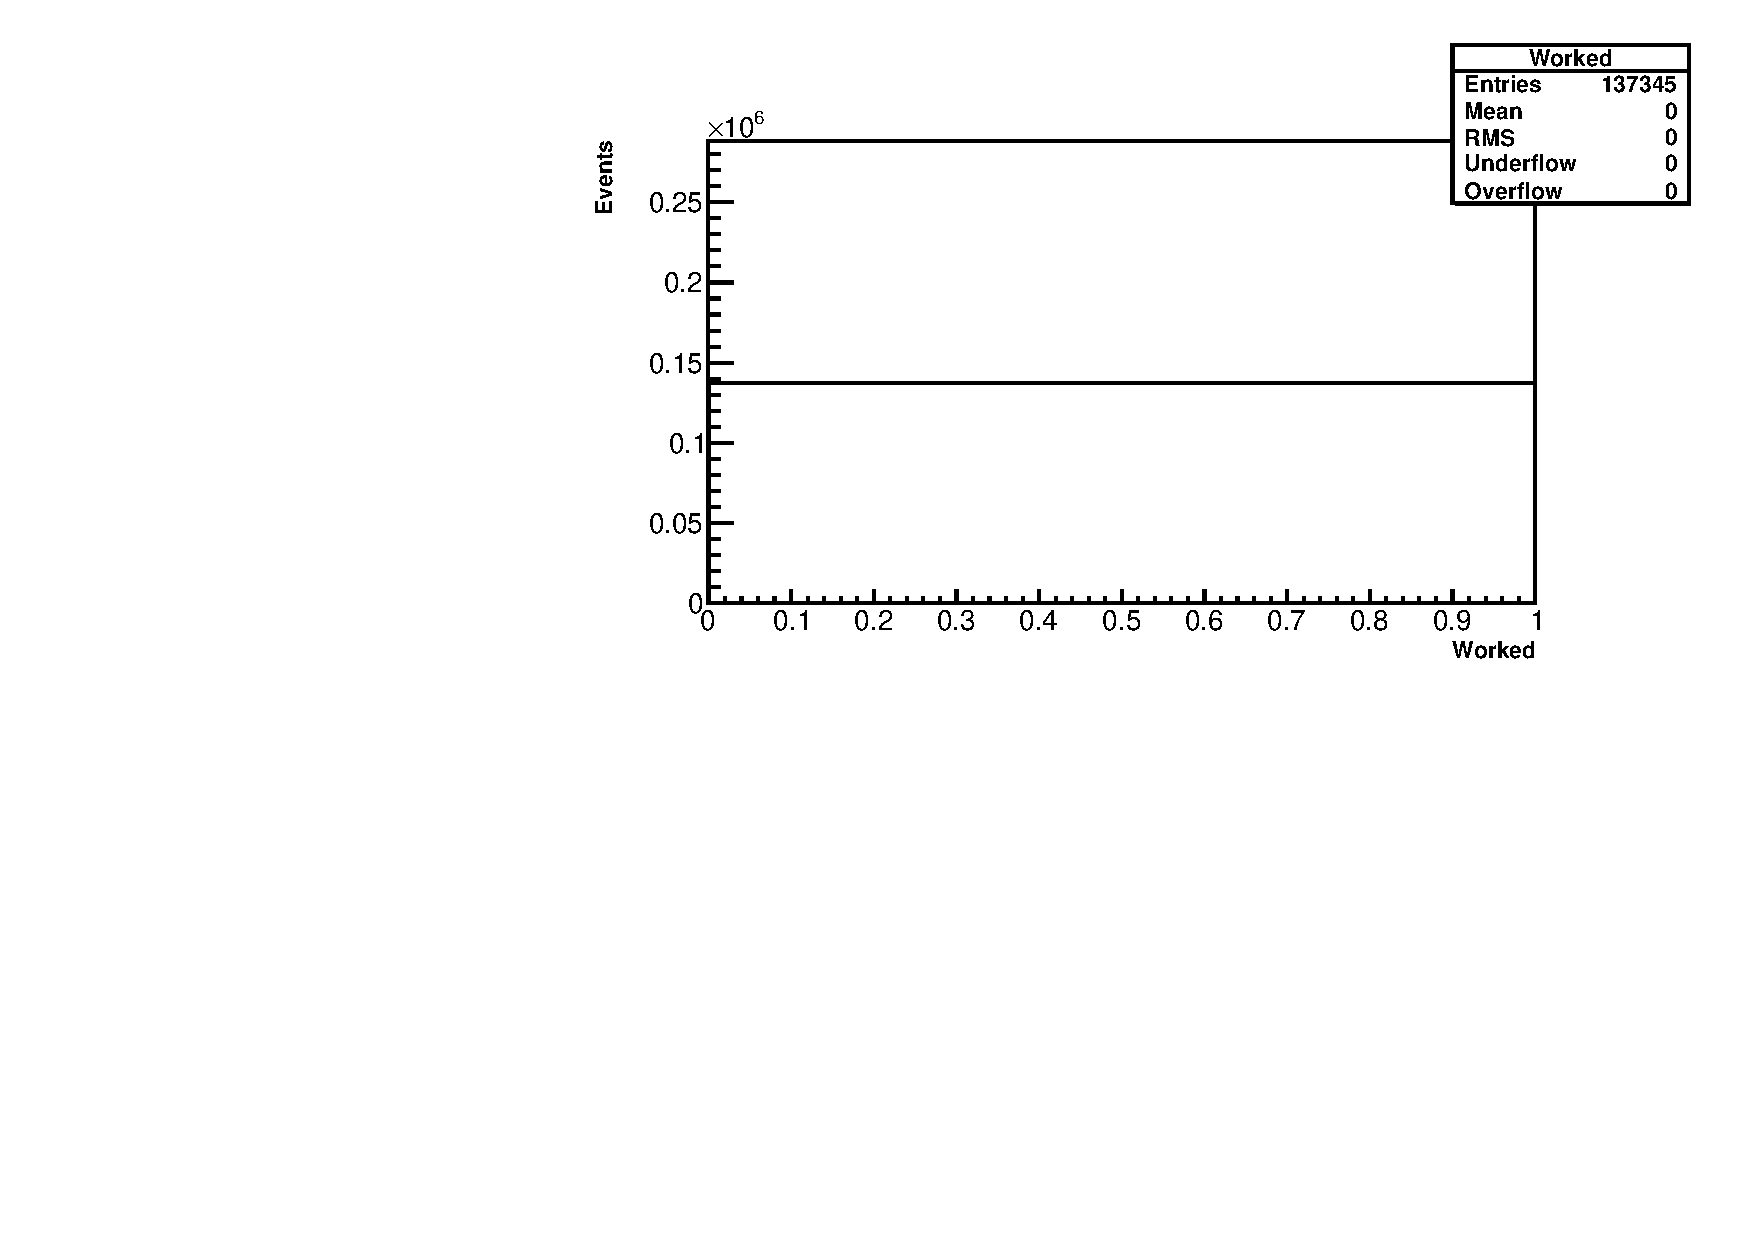
\includegraphics[width=1\textwidth]{WorkedEvents} 
        \caption{Number of events that passed the track fitting, with no cuts applied.}
        \label{fig:worked}
    \end{subfigure}
    
    \begin{subfigure}[]{0.7\textwidth}
        \centering
        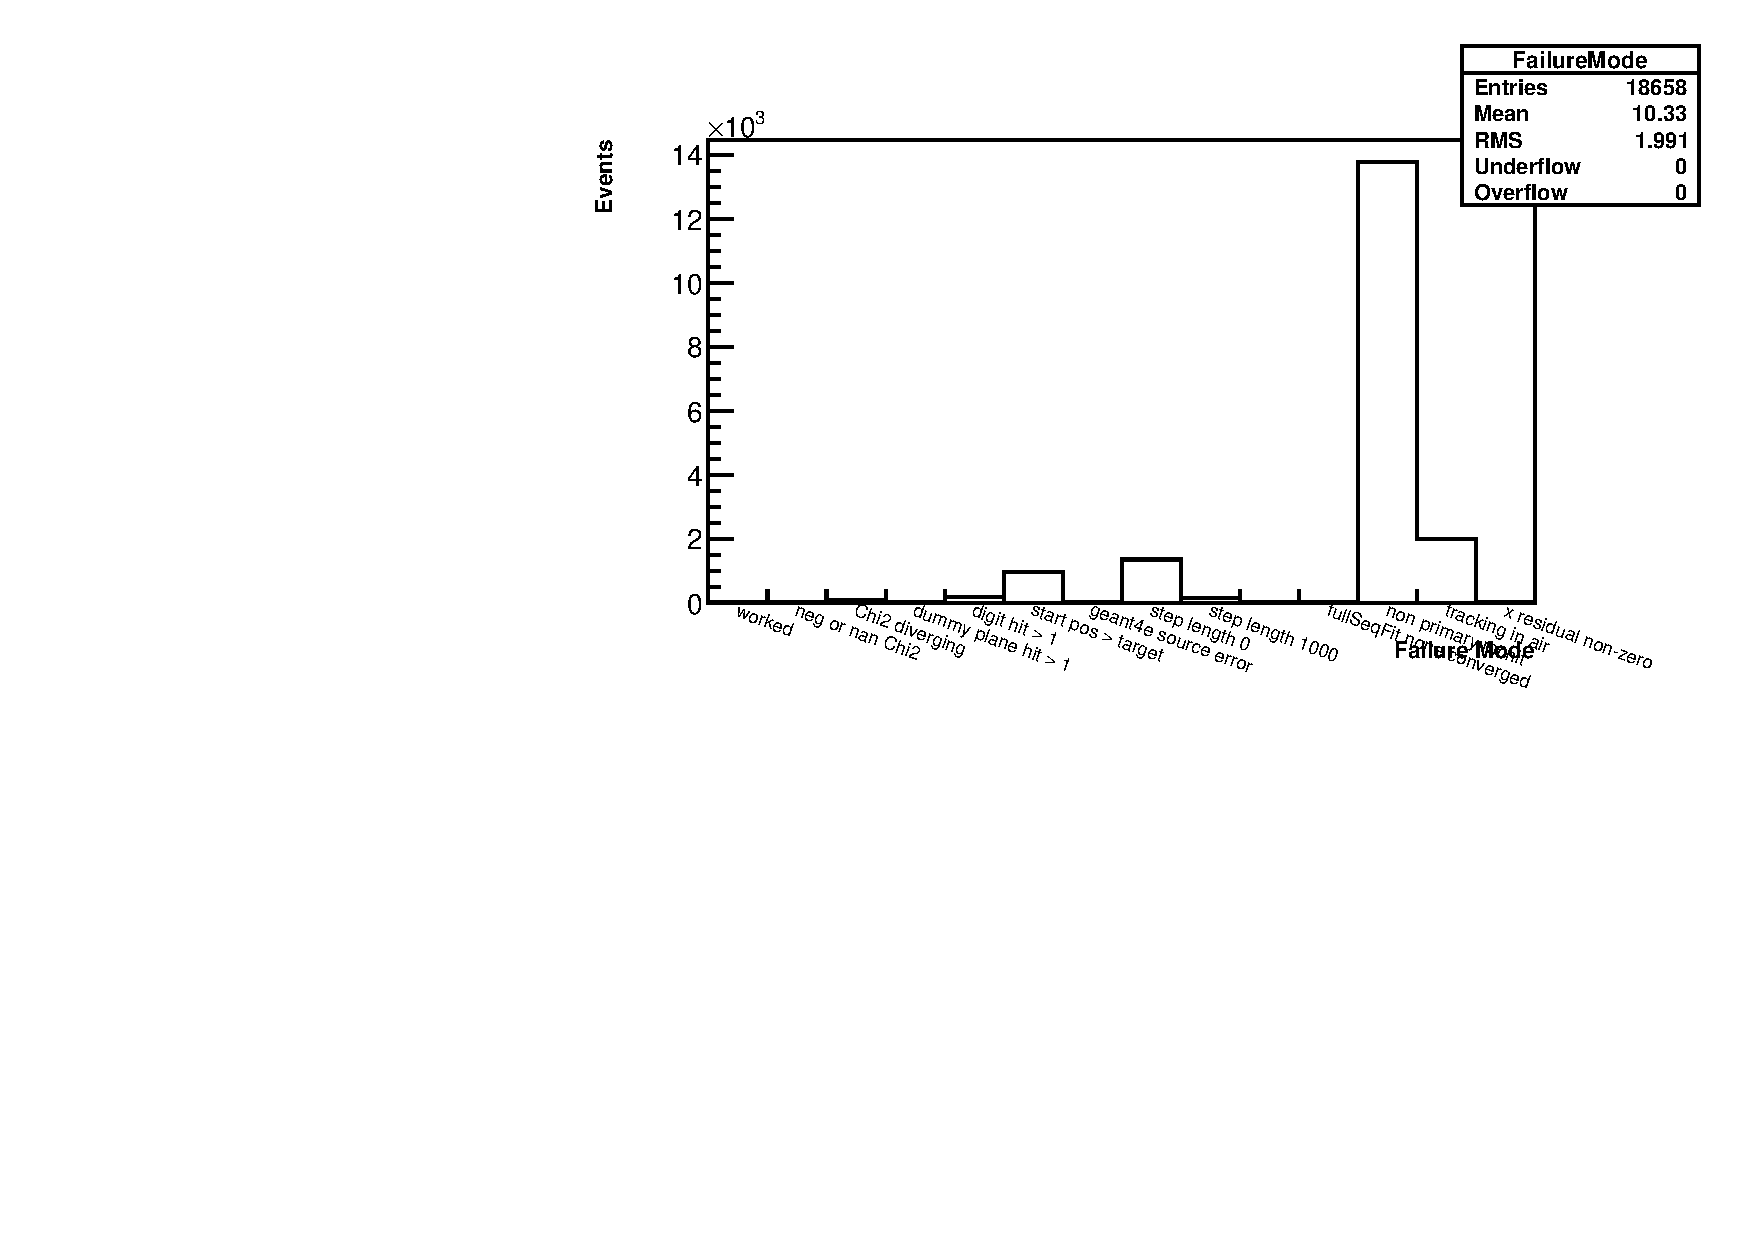
\includegraphics[width=1\textwidth]{FailedEventsUnzoomed} 
        \caption{Failure modes for the track reconstruction. Most ``failures'' are Geant issues.}
    \end{subfigure}

    \begin{subfigure}[]{0.7\textwidth}
        \centering
        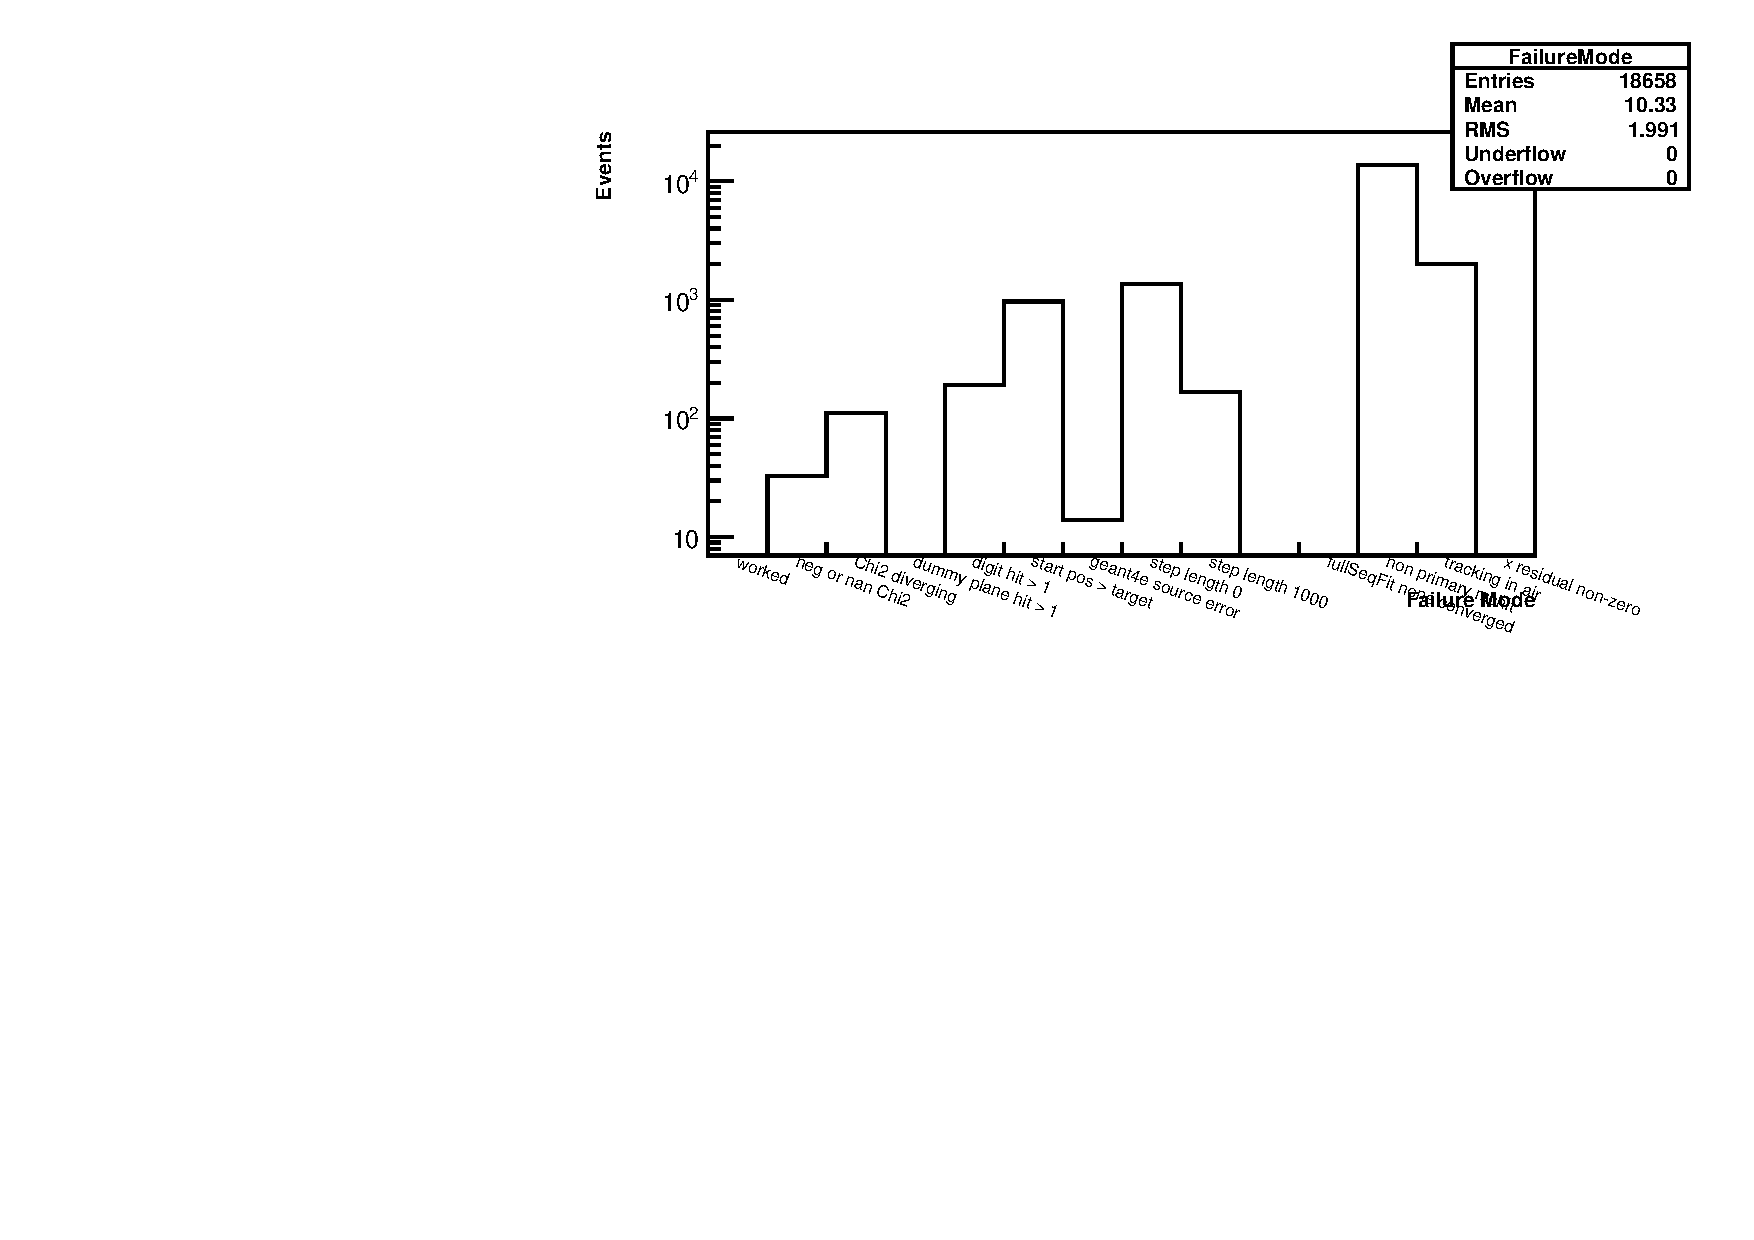
\includegraphics[width=1\textwidth]{FailedEventsLog} 
        \caption{Log plot of the failure modes. The first two failure mode bins are the most important.}
    \end{subfigure}

    \caption{The number of events that passed and failed the Geane track fitting.}
\end{figure}



\begin{figure}
    \centering
    \begin{subfigure}[]{0.7\textwidth}
        \centering
        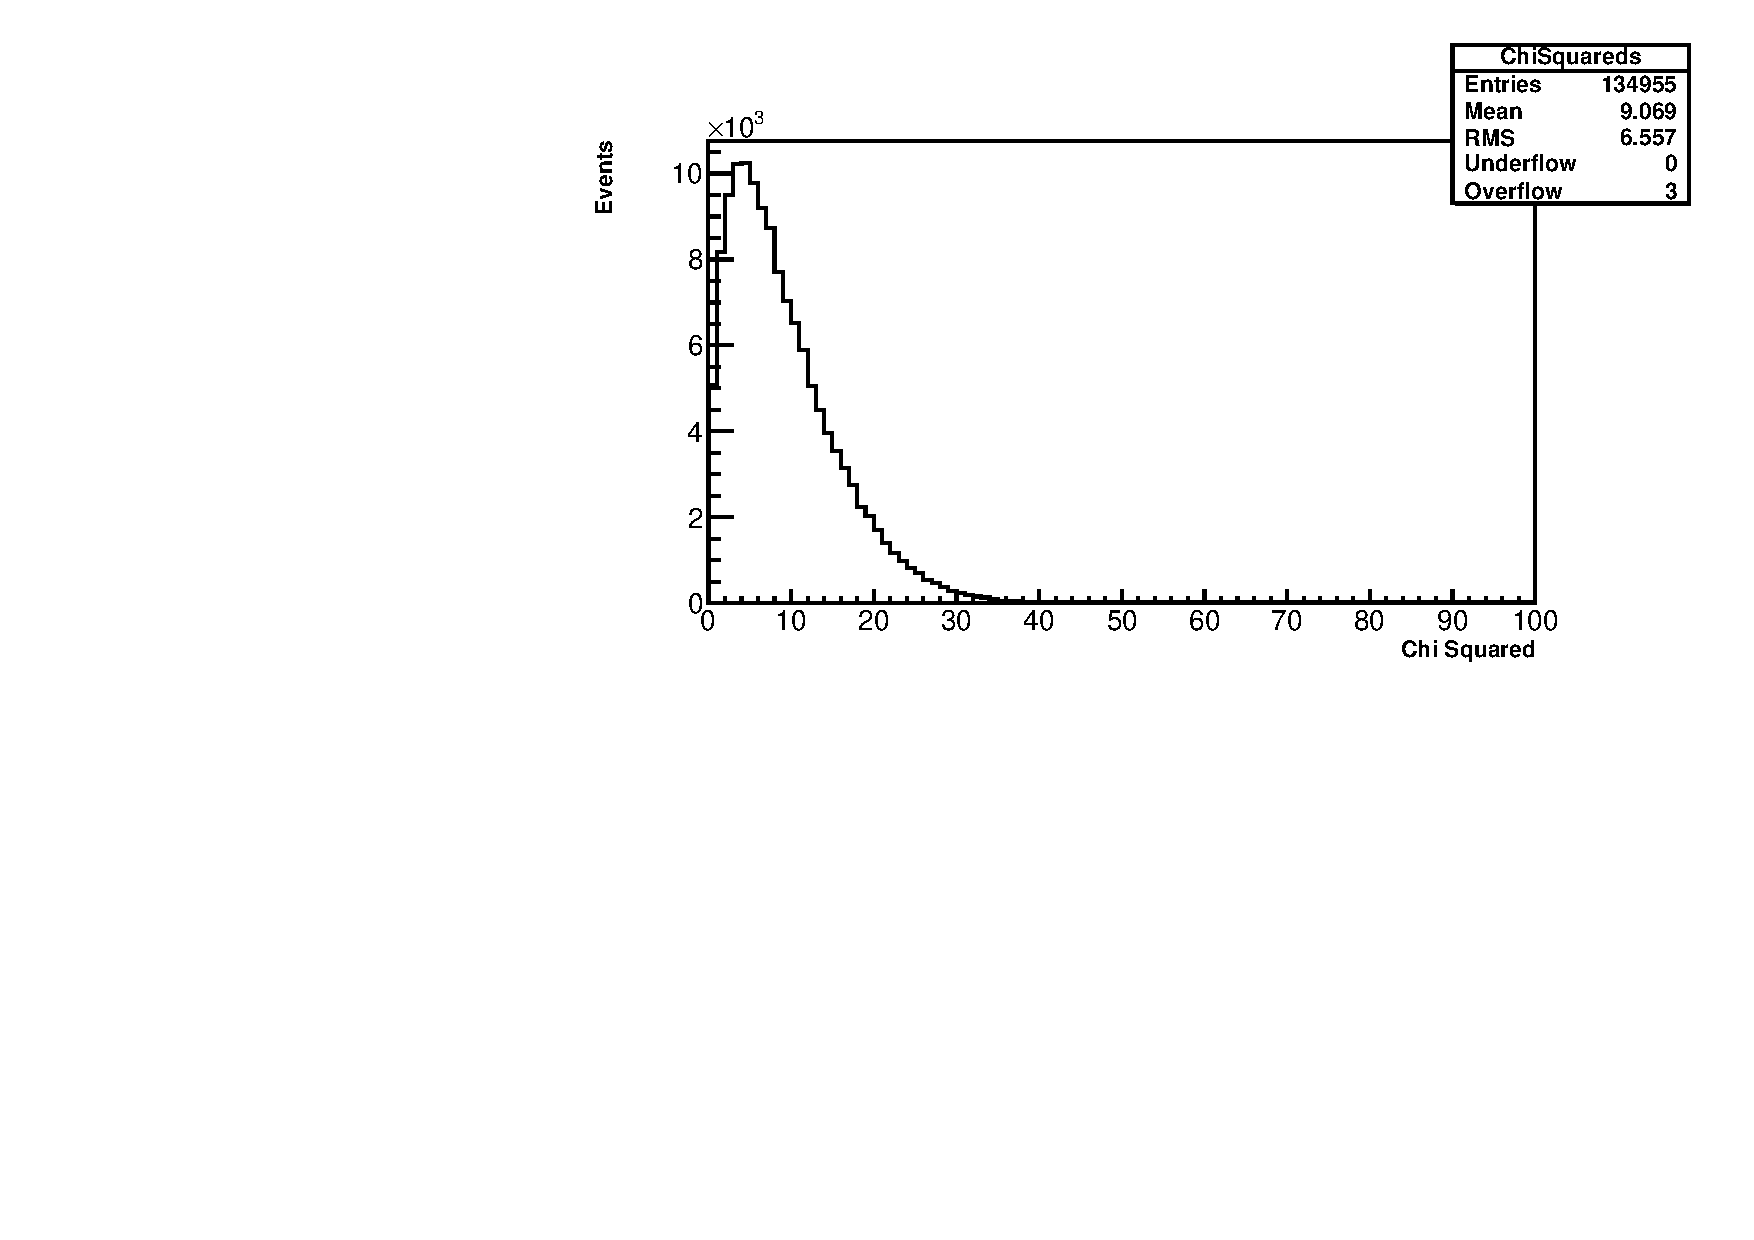
\includegraphics[width=1\textwidth]{chi2} 
        \caption{Distribution of $\chi^{2}$s for all tracks. Comprised of separate $\chi^{2}$ distributions with degrees of freedom equal to the number of planes hit minus 5.}
    \end{subfigure}
    
    \begin{subfigure}[]{0.7\textwidth}
        \centering
        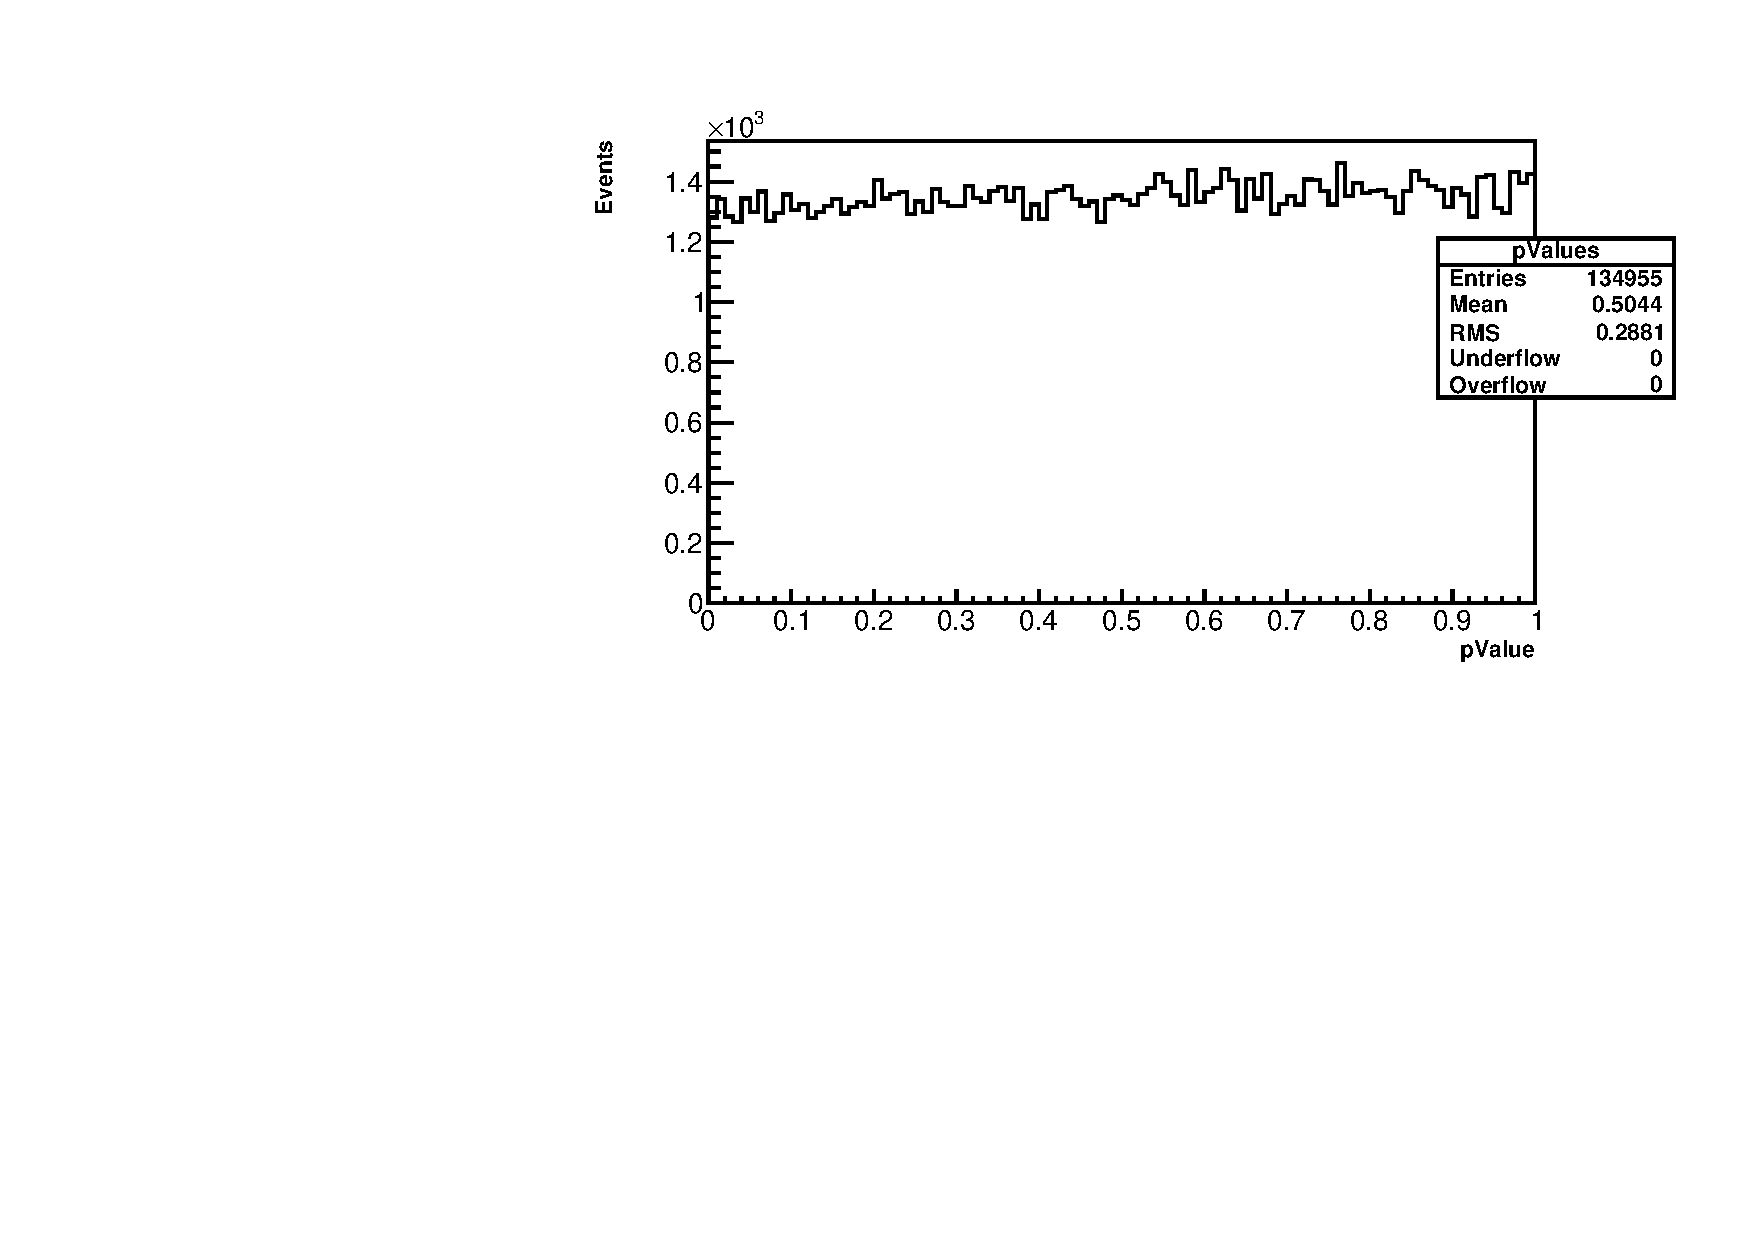
\includegraphics[width=1\textwidth]{pValueUnzoomed} 
        \caption{P-value distribution for tracks. Very nearly uniform, showing tracking is working as expected.}
    \end{subfigure}

    \begin{subfigure}[]{0.7\textwidth}
        \centering
        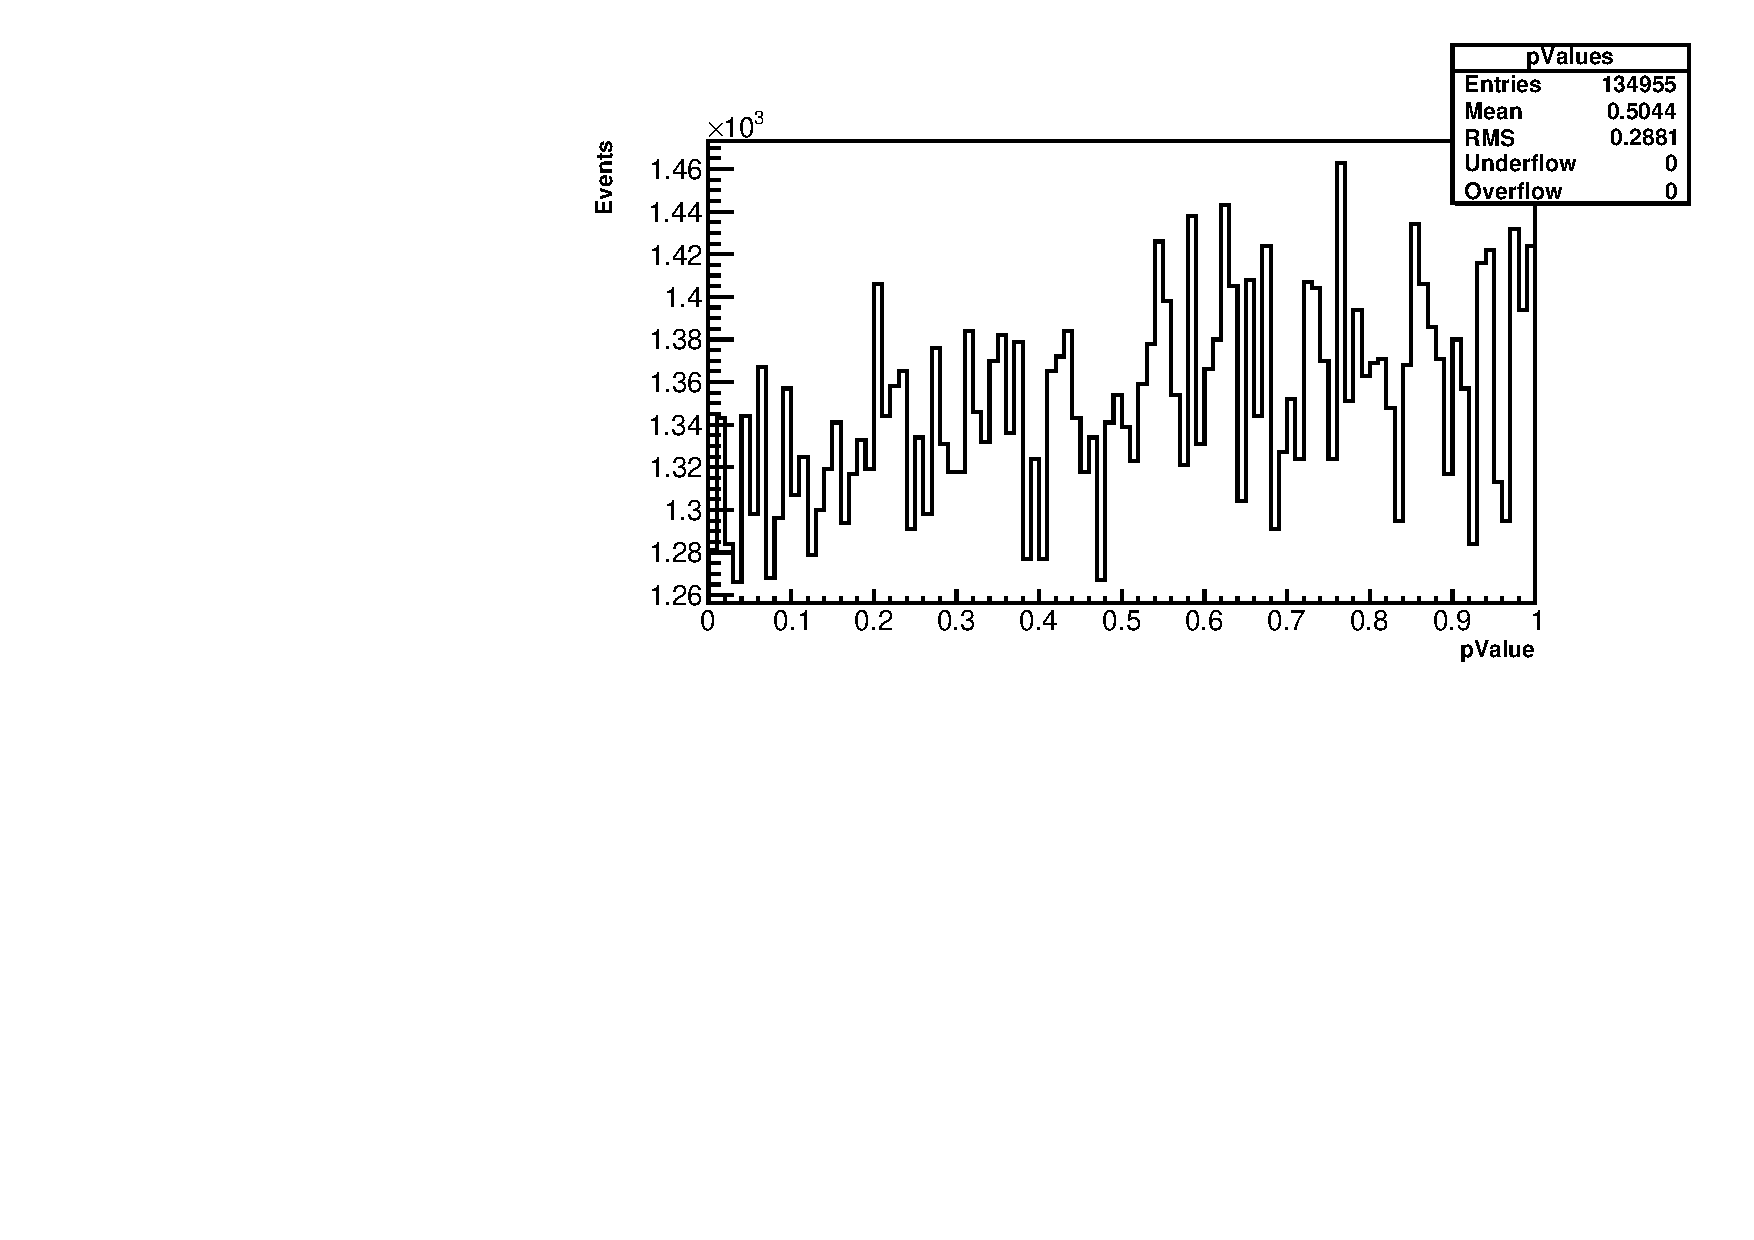
\includegraphics[width=1\textwidth]{pValueZoomed} 
        \caption{P-value distribution zoomed in. A slight rise towards 1 can be seen.}
    \end{subfigure}

    \caption{$\chi^{2}$ and p-value distributions for all tracks. There are less entries than in \ref{fig:worked} due to the energy cut of 3 MeV.}
\end{figure}



\begin{figure}
    \centering
    \begin{subfigure}[]{0.65\textwidth}
        \centering
        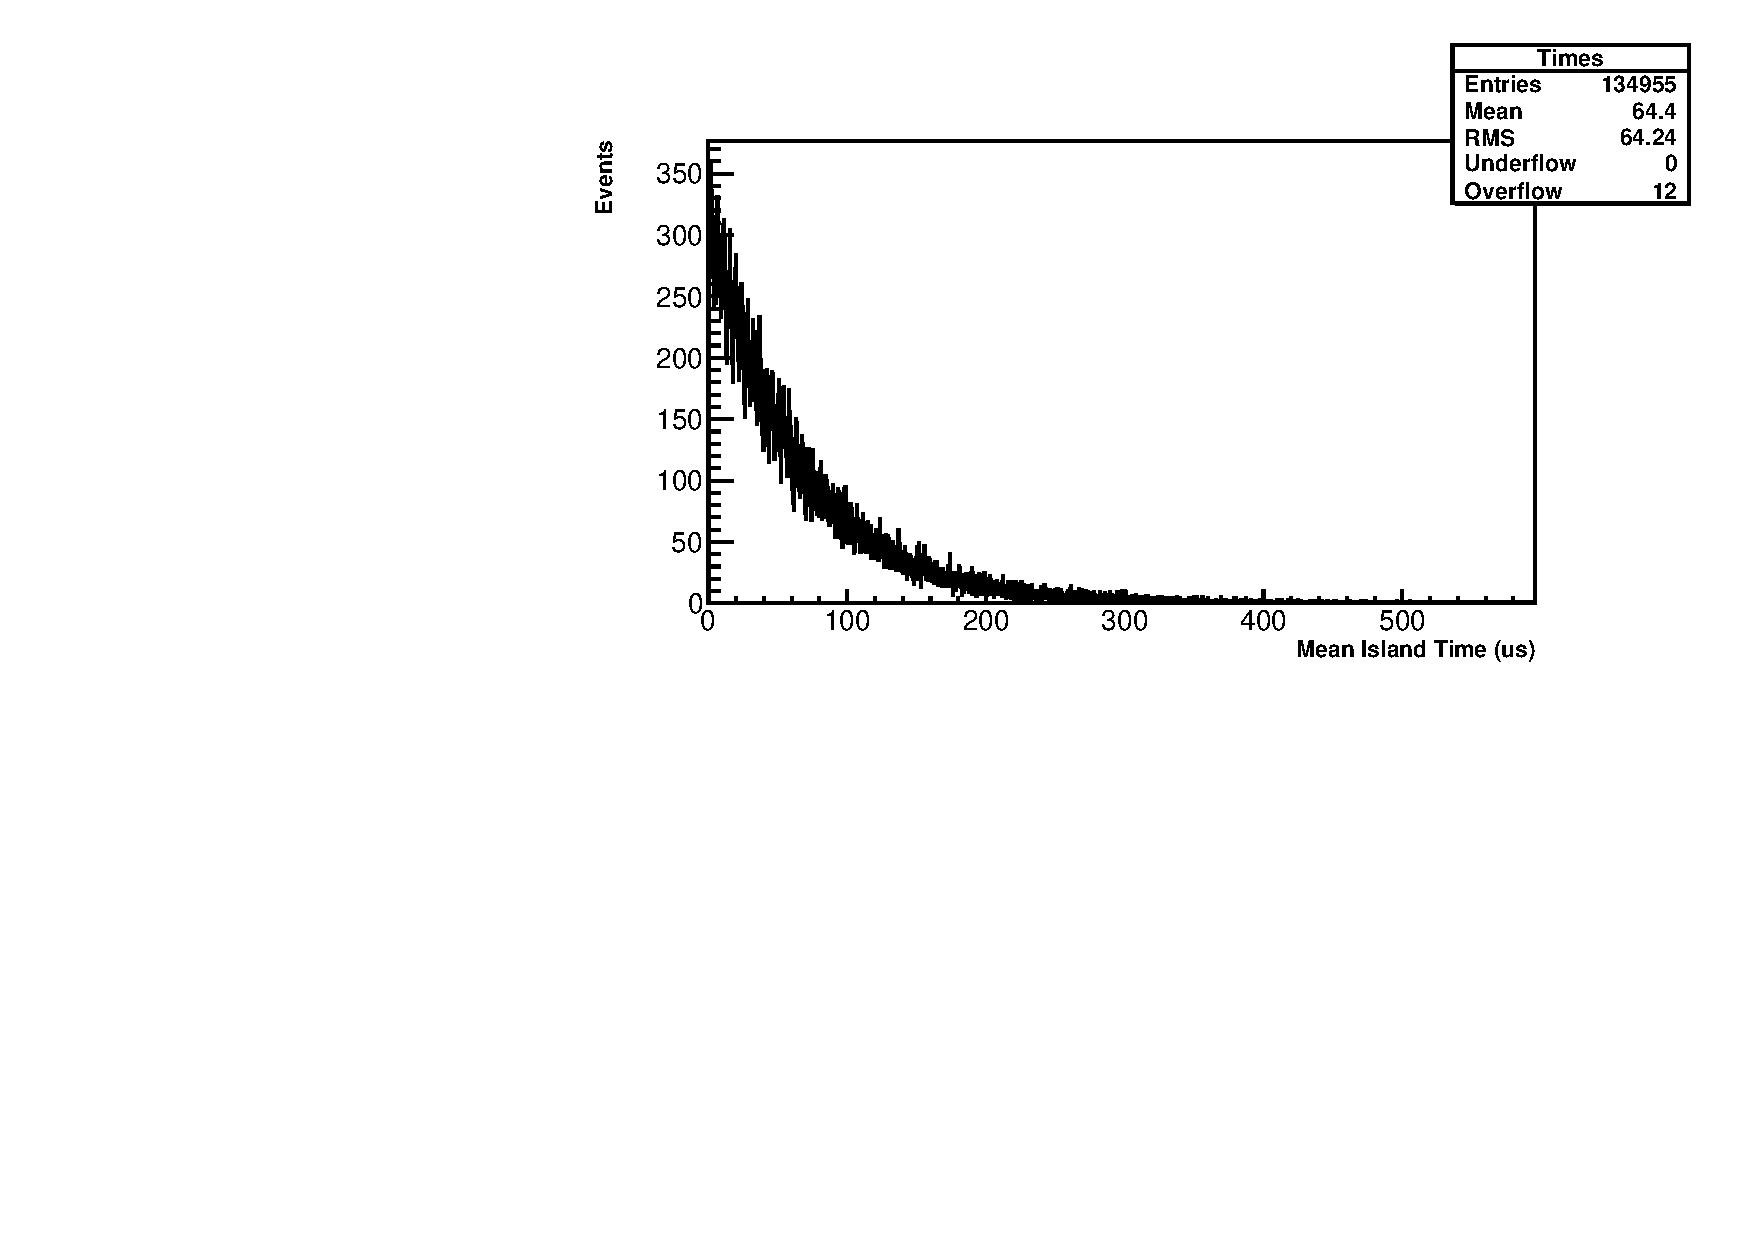
\includegraphics[width=1\textwidth]{Times} 
        \caption{Mean island times for fitted events from the mdc1 simulation. The cbo can just barely be seen.}
    \end{subfigure}
    
    \begin{subfigure}[]{0.65\textwidth}
        \centering
        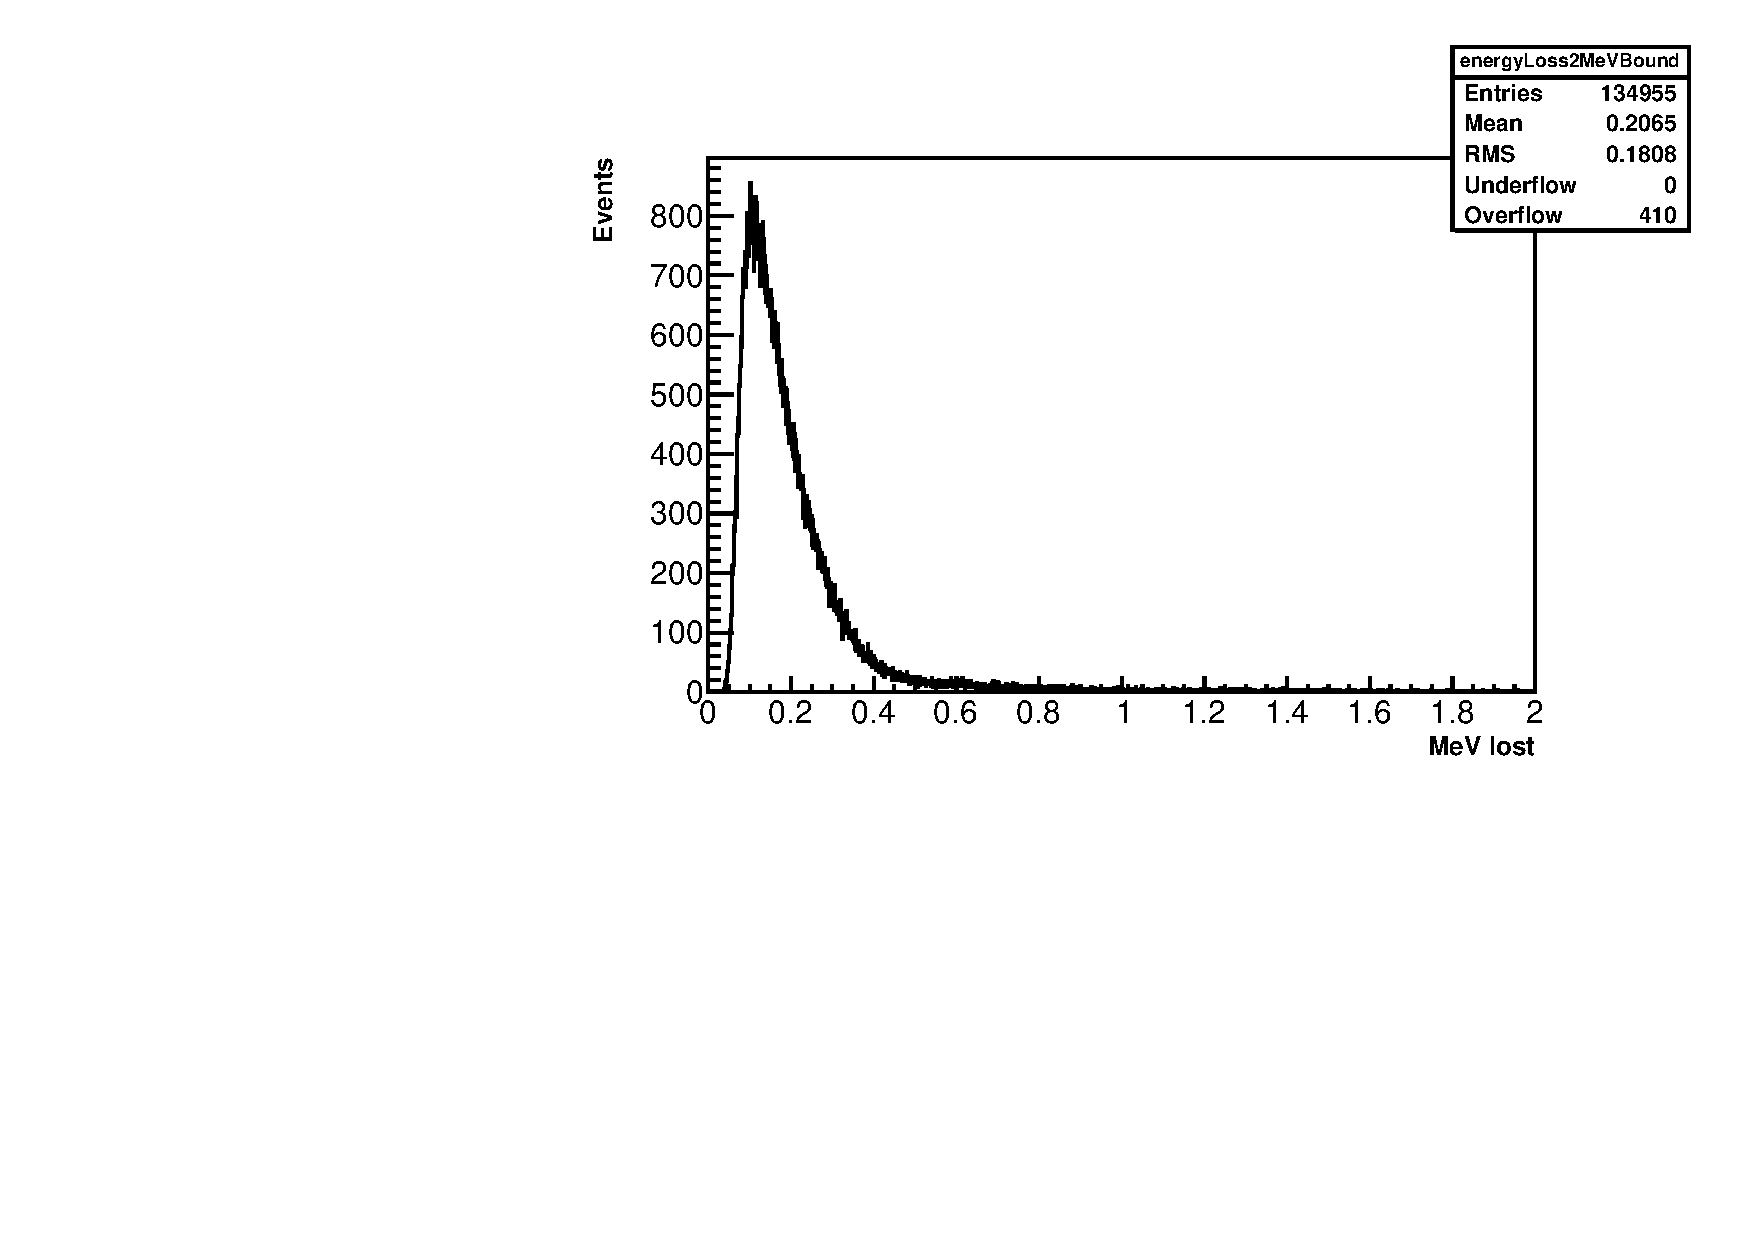
\includegraphics[width=1\textwidth]{trueEnergyLoss} 
        \caption{True energy loss between the first and last hit in the tracker. Peaks at about 120 keV with a mean of about 200 keV.}
    \end{subfigure}

    \begin{subfigure}[]{0.65\textwidth}
        \centering
        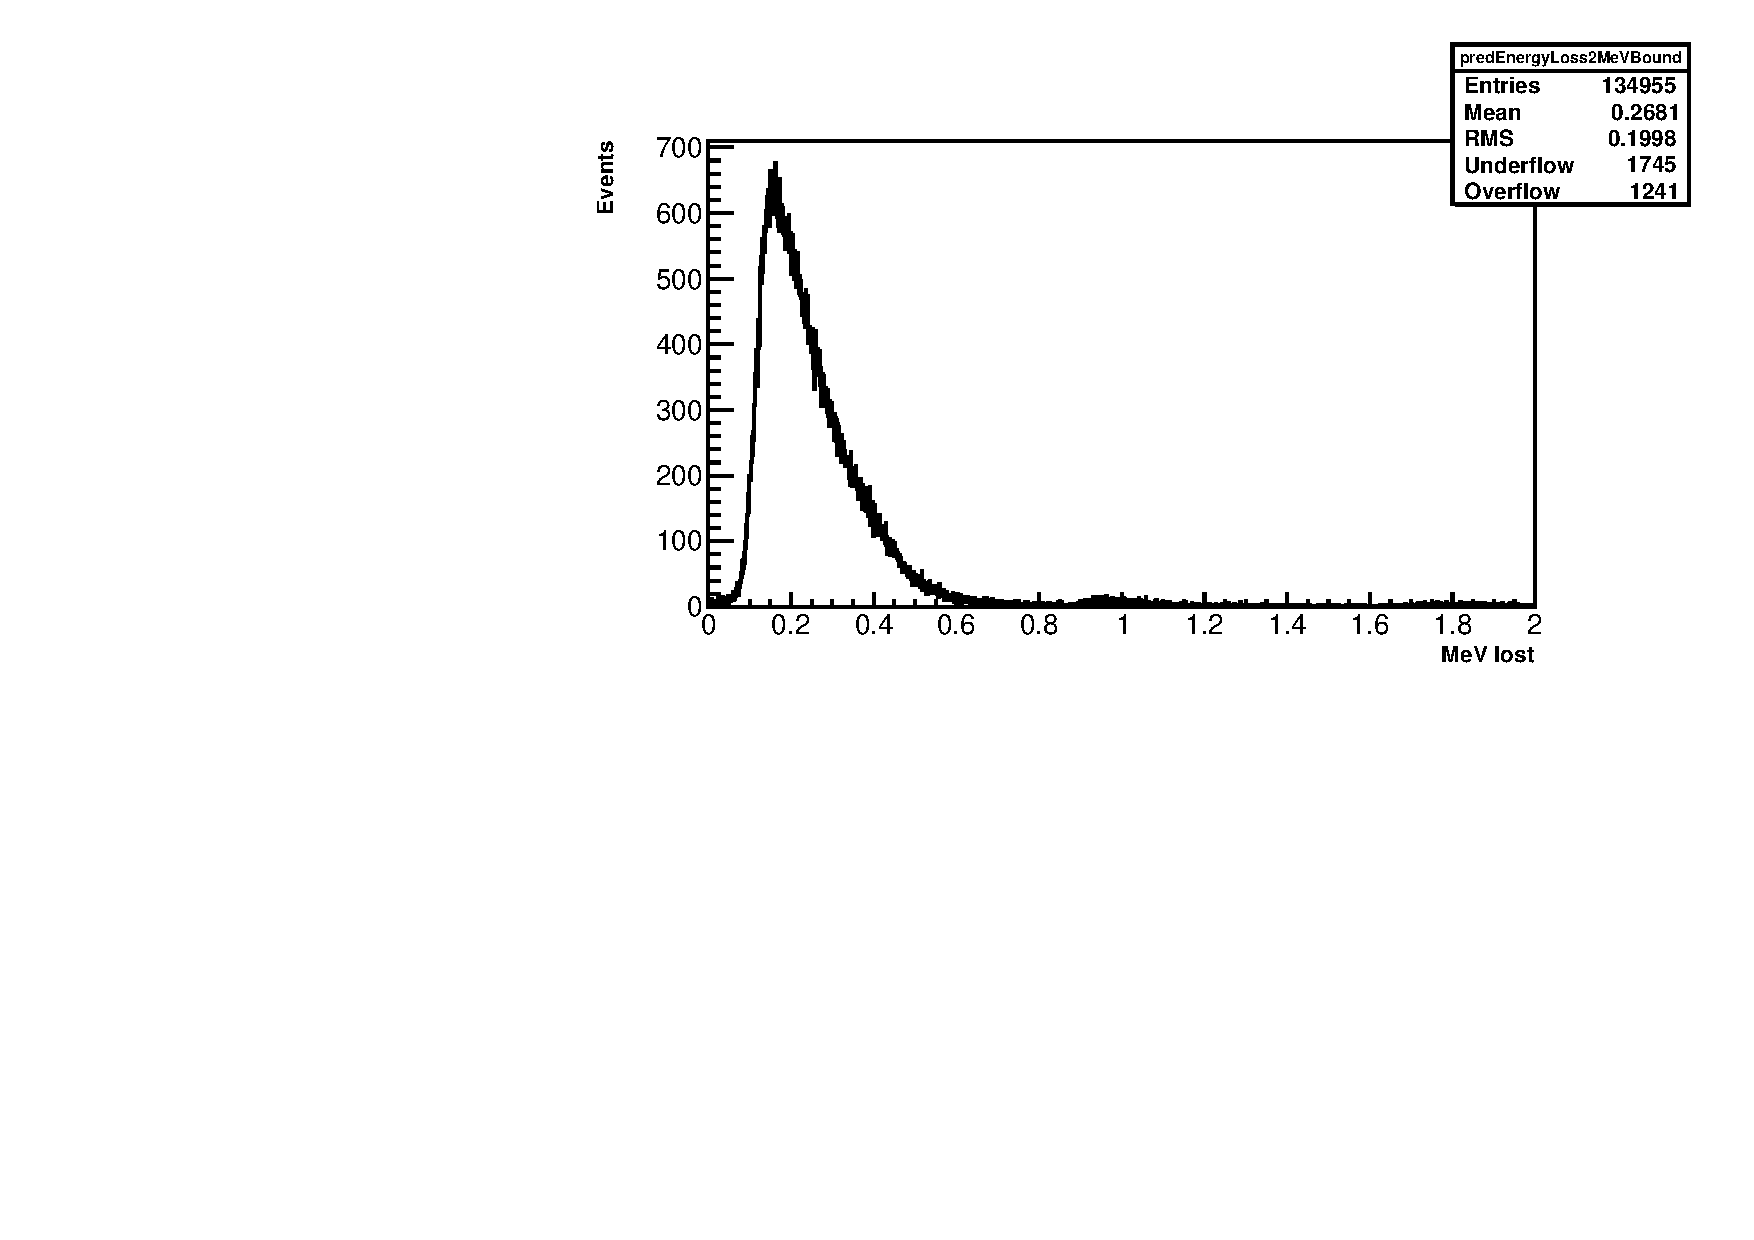
\includegraphics[width=1\textwidth]{predEnergyLoss} 
        \caption{Predicted energy loss from Geane fitting. Peaks at about 150 keV with a mean of about 270 keV. There is a slight overestimation of energy loss from truth. This is pretty negligble, but can probably be improved if necessary.}
    \end{subfigure}

    \caption{Energy and time information of the fitted tracks.}
\end{figure}



\begin{figure}
    \centering
    \begin{subfigure}[]{0.6\textwidth}
        \centering
        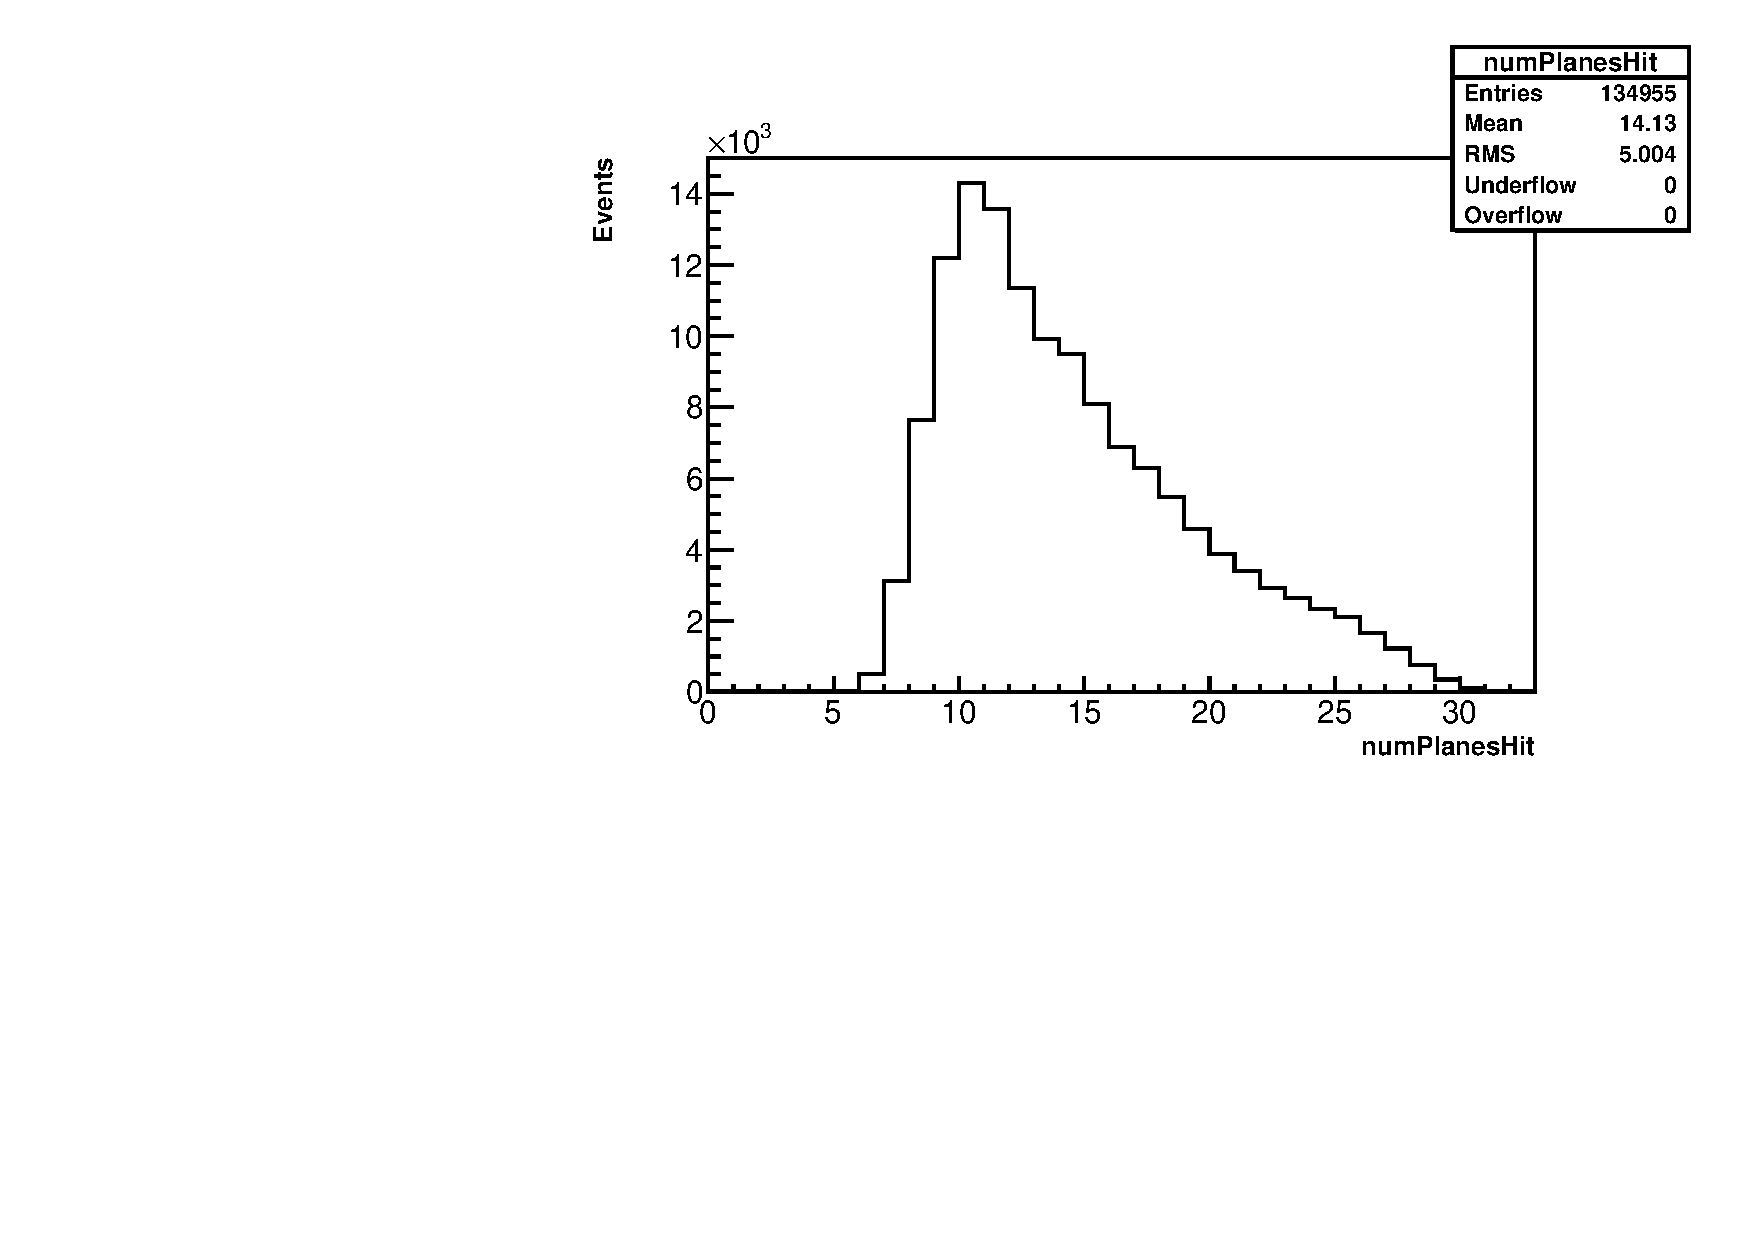
\includegraphics[width=1\textwidth]{numPlanesHit} 
        \caption{Number of planes hit per track. Peaks at 11 and falls off steadily.}
    \end{subfigure}
    
    \begin{subfigure}[]{0.6\textwidth}
        \centering
        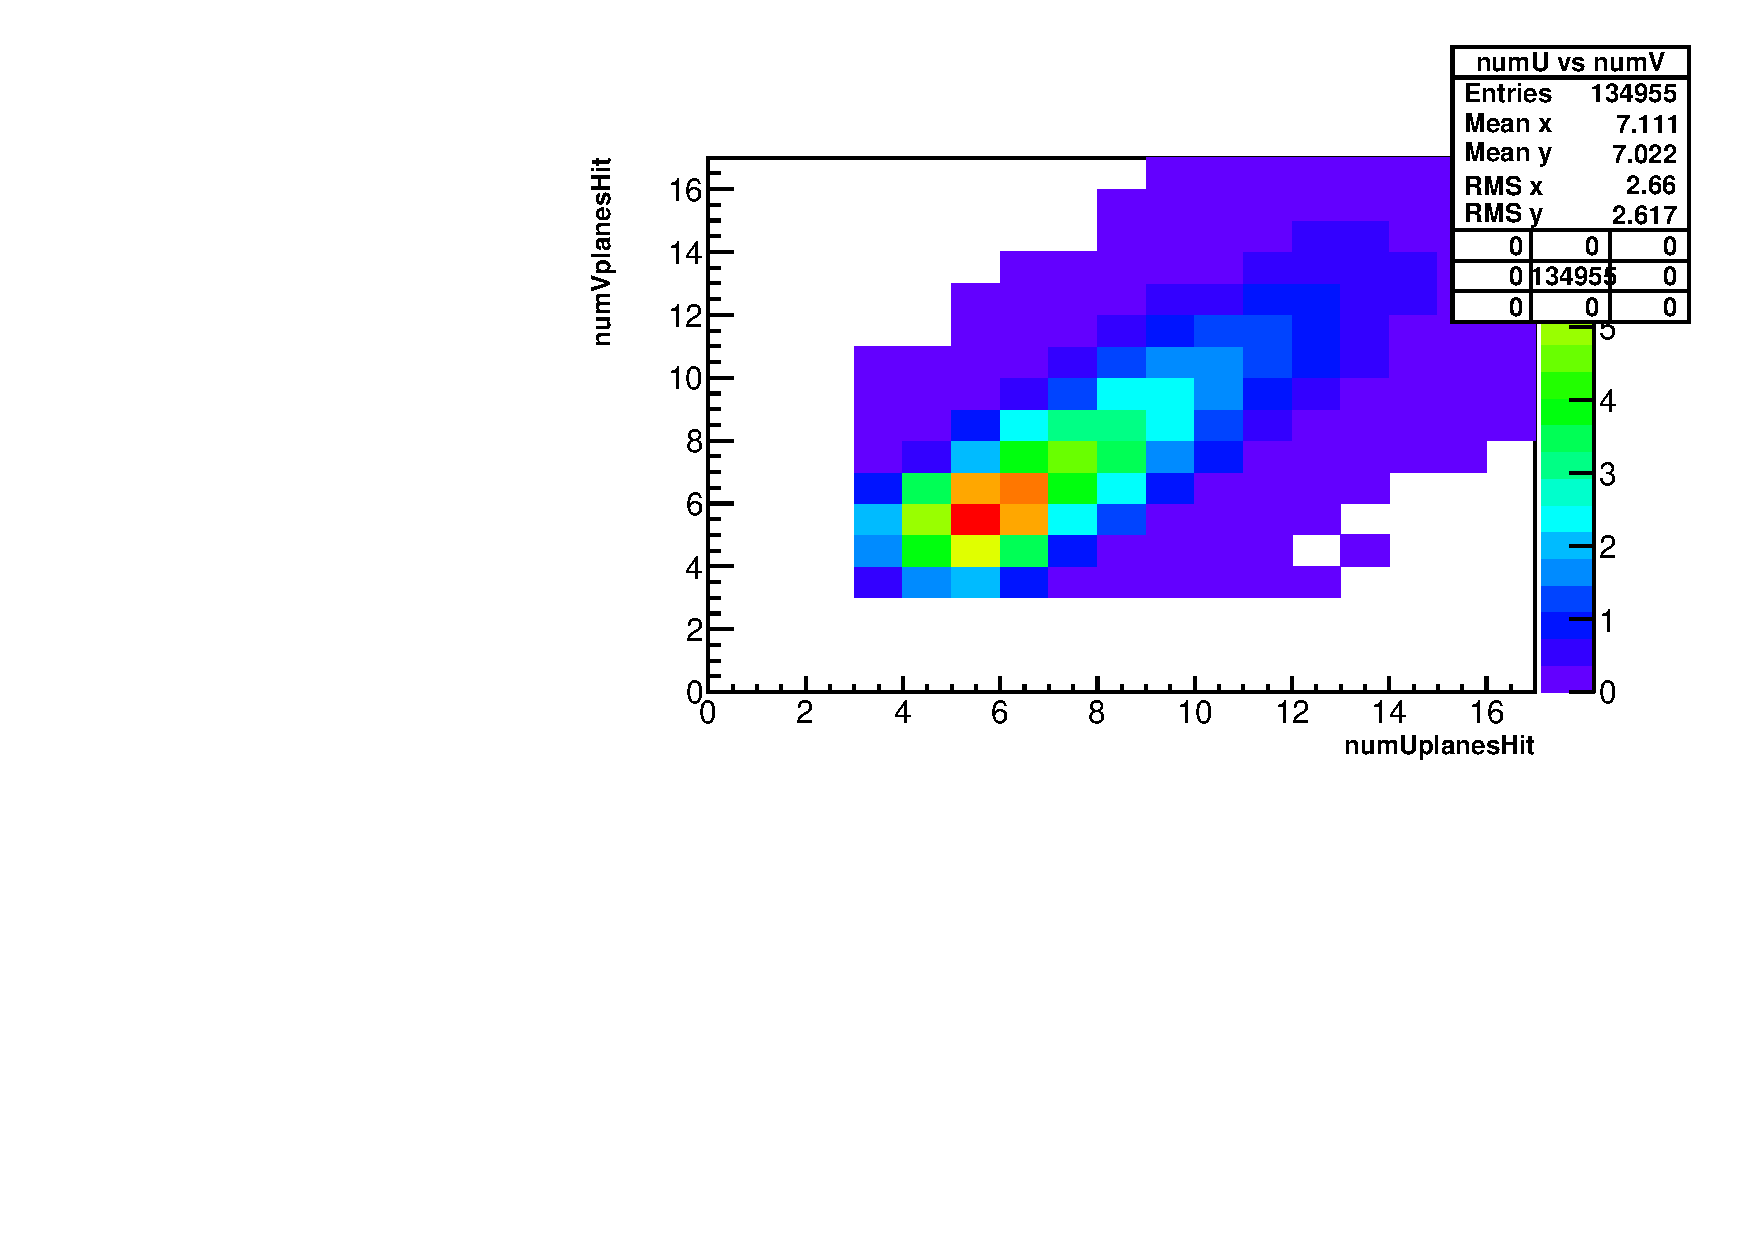
\includegraphics[width=1\textwidth]{numUnumV} 
        \caption{Number of U planes hit vs the number of V planes hit.}
    \end{subfigure}

    \begin{subfigure}[]{0.6\textwidth}
        \centering
        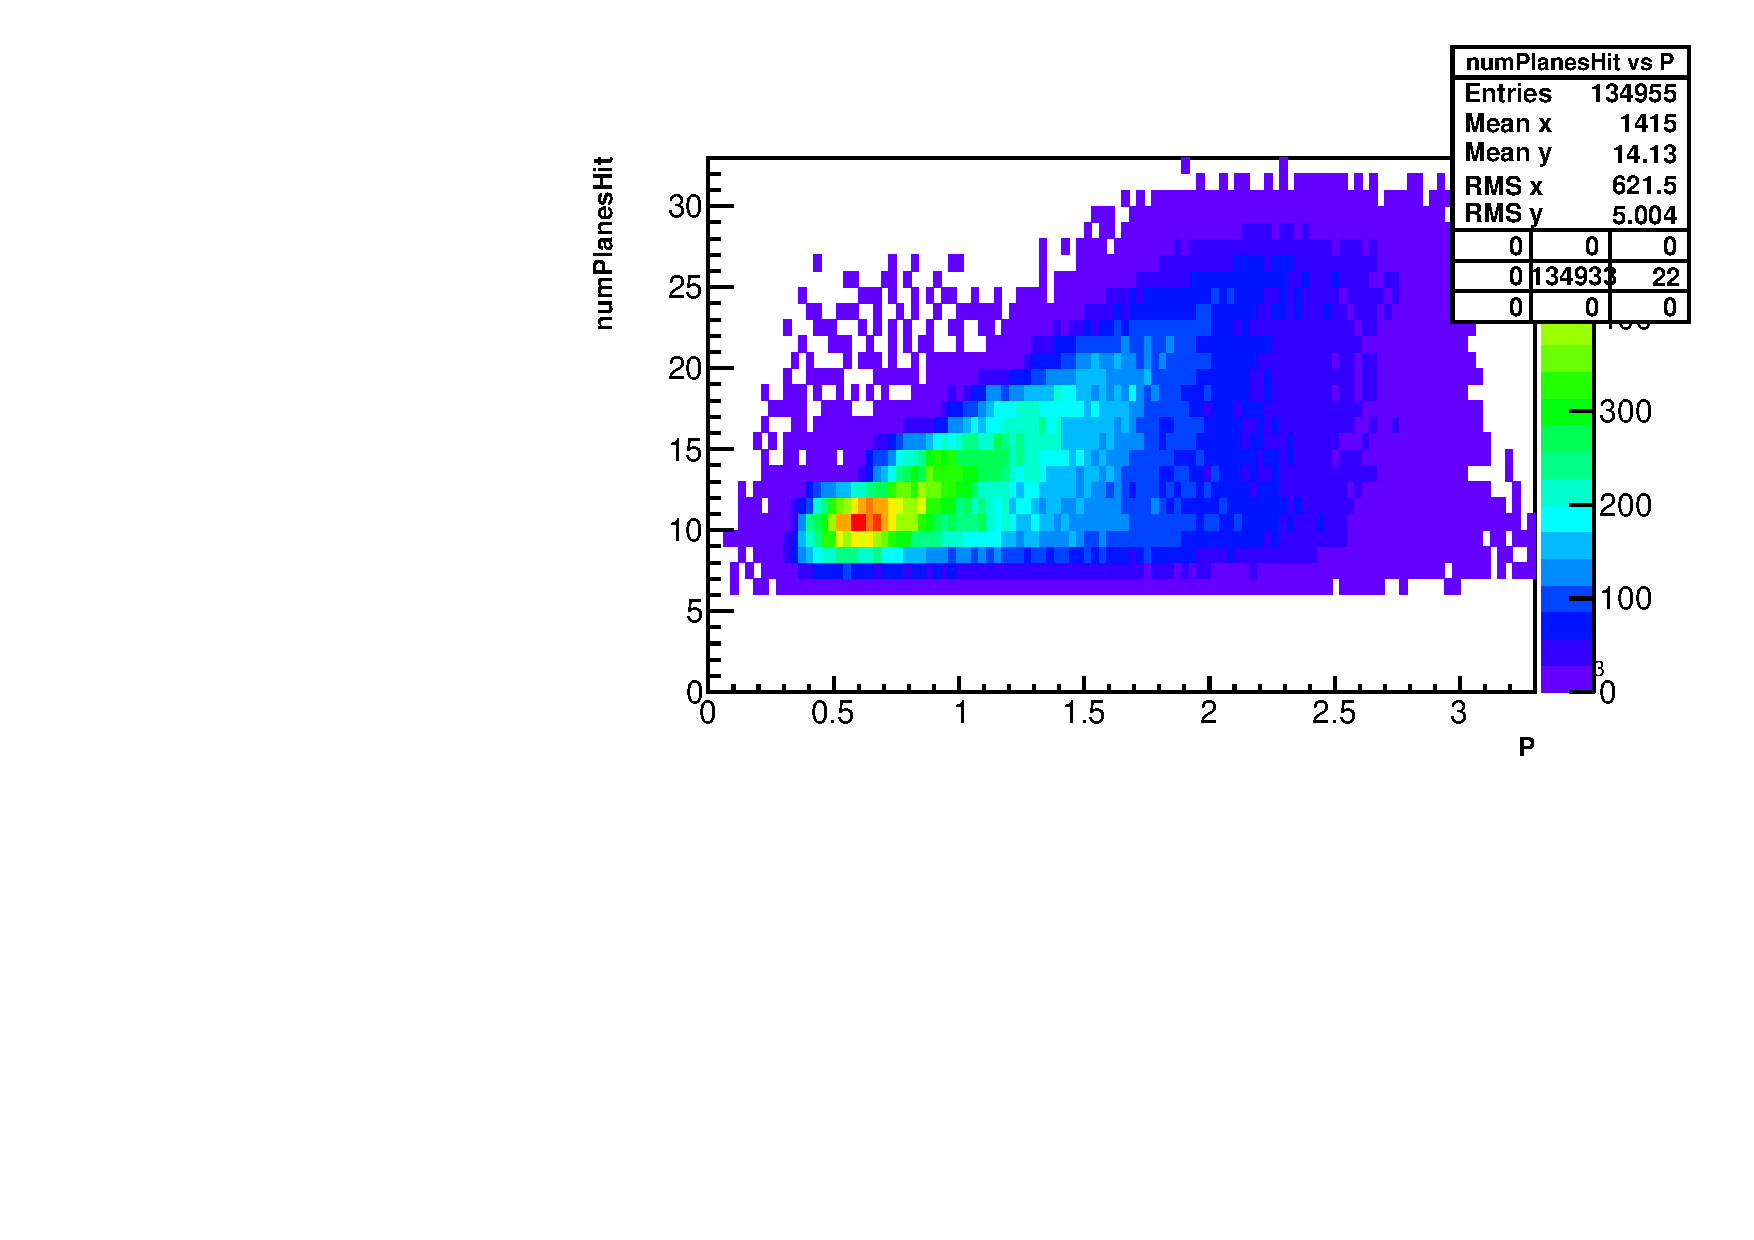
\includegraphics[width=1\textwidth]{numHitvsP} 
        \caption{Number of planes hit vs track momentum. These variables are very correlated, the higher the momentum of the track, the more likely it is to hit more planes.}
    \end{subfigure}

    \caption{Number of planes hit information.}
\end{figure}



\begin{figure}
    \centering
    \begin{subfigure}[]{0.8\textwidth}
        \centering
        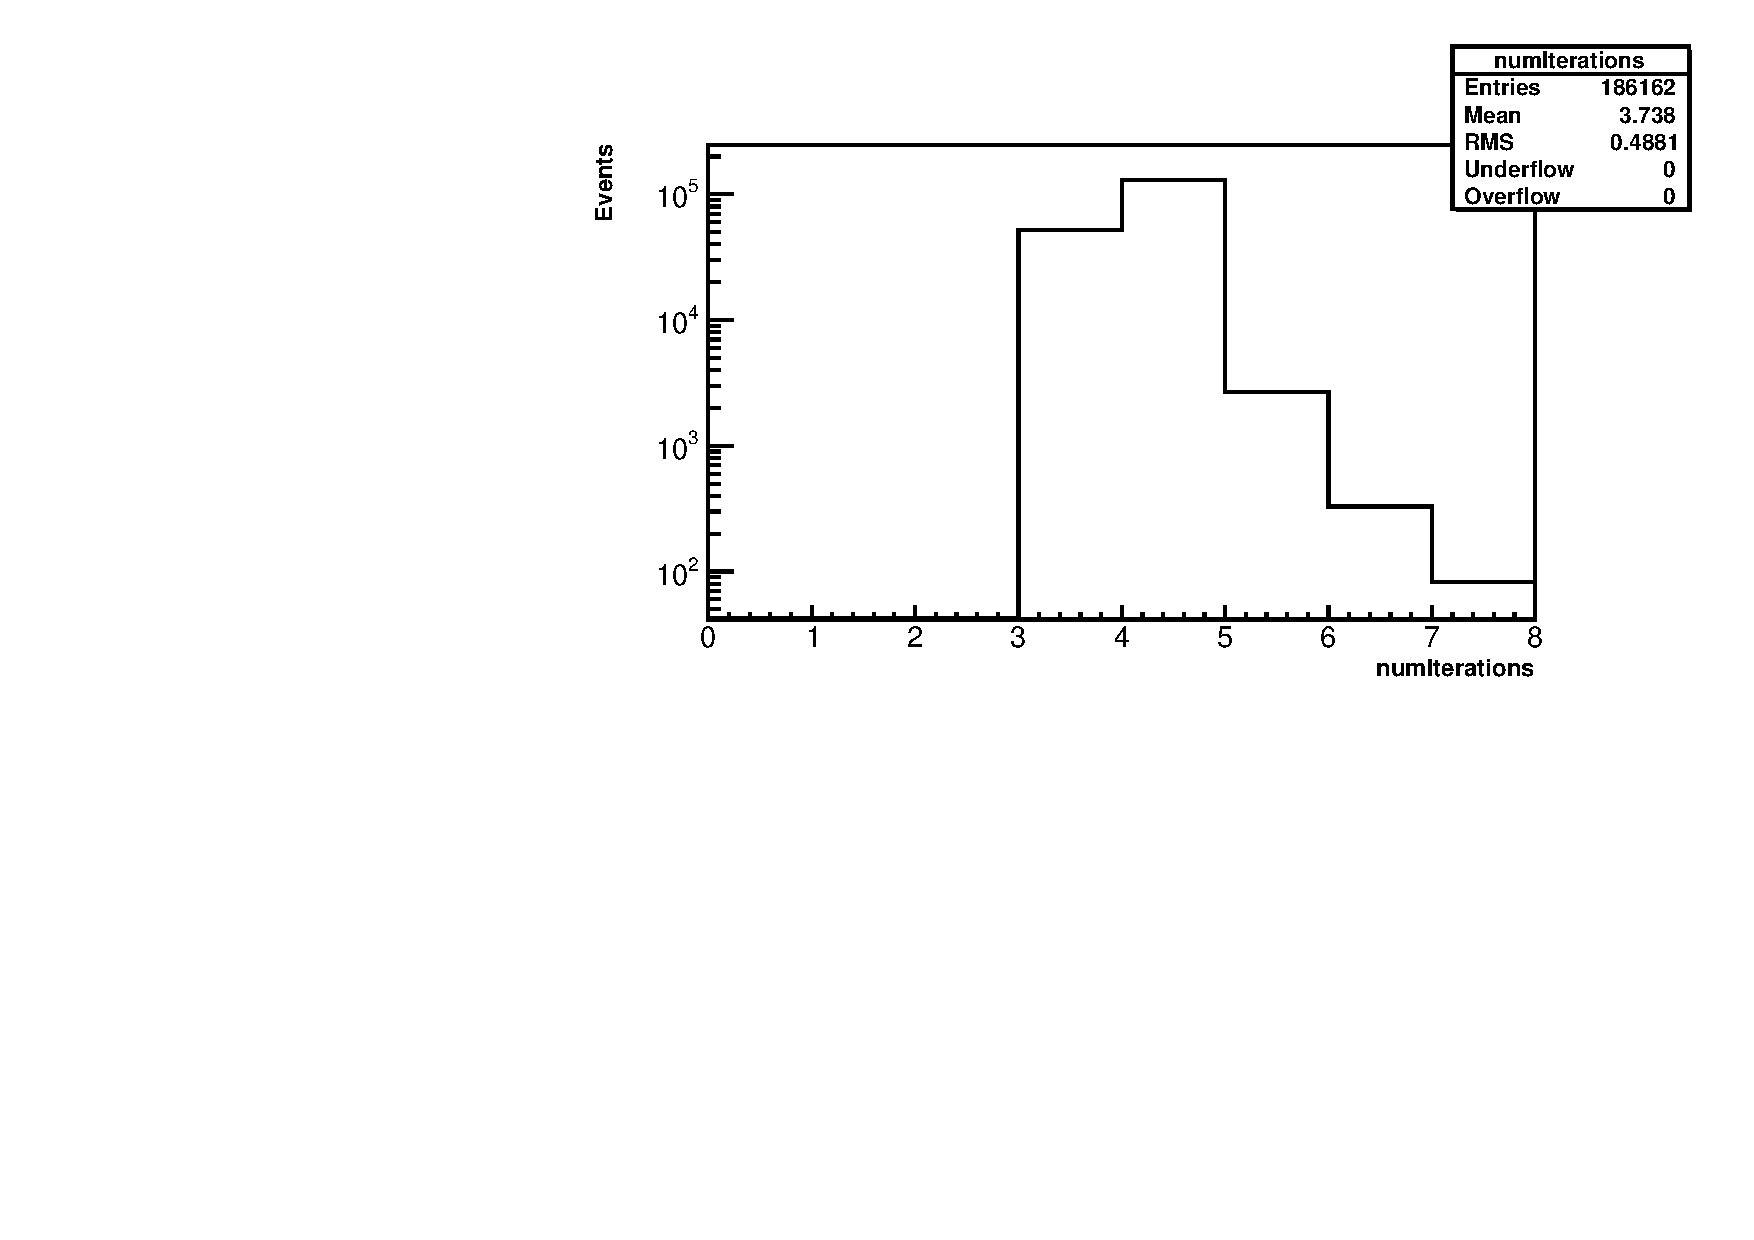
\includegraphics[width=1\textwidth]{numIterations} 
        \caption{Number of iterations to fit the track. Peaks at 4 with not less than 3 iterations.}
    \end{subfigure}
    
    \begin{subfigure}[]{0.8\textwidth}
        \centering
        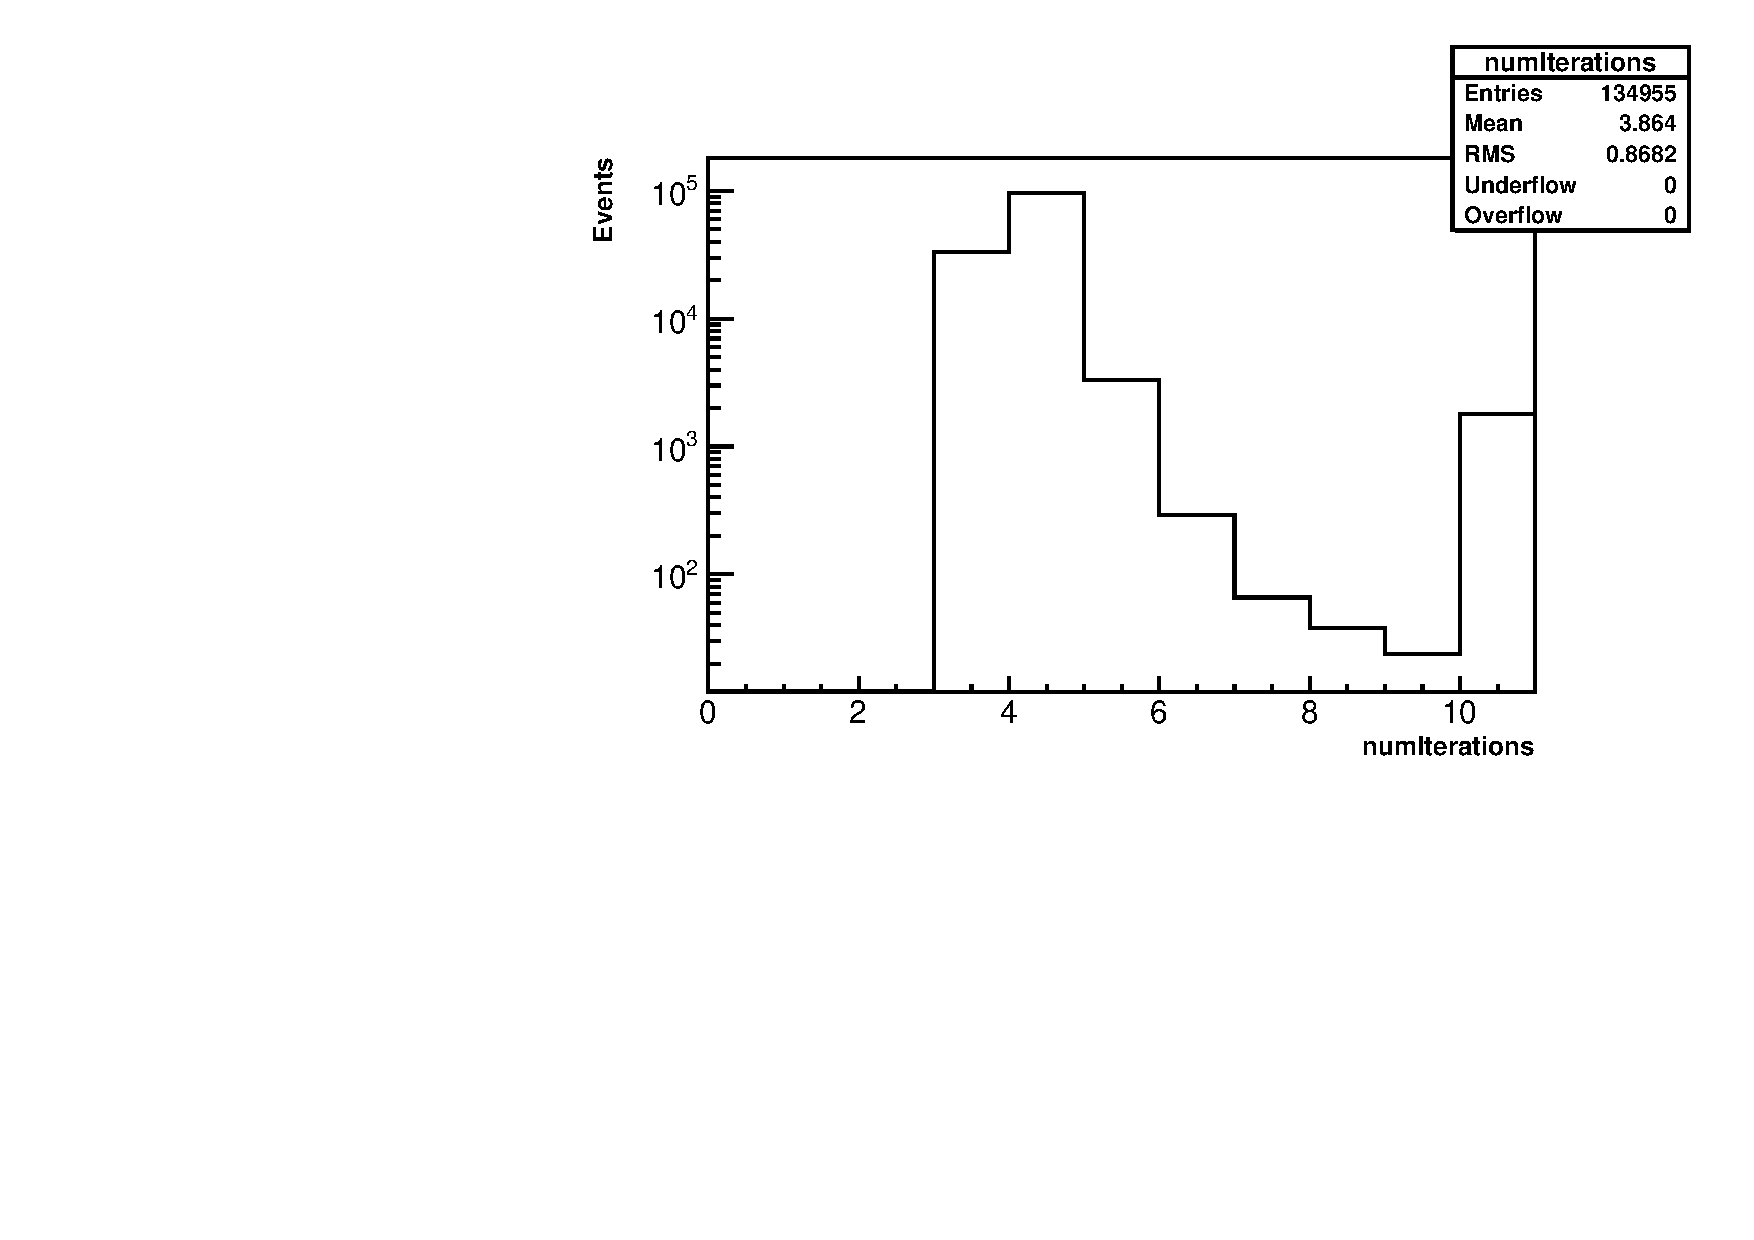
\includegraphics[width=1\textwidth]{numIterationsLog} 
        \caption{Number of iterations log plot. The number of iterations is manually cut off at 10, which is why there is an increase in the last bin and no overflows.}
    \end{subfigure}

    \caption{Number of iterations information.}
\end{figure}



\begin{figure}
    \centering
    \begin{subfigure}[]{0.65\textwidth}
        \centering
        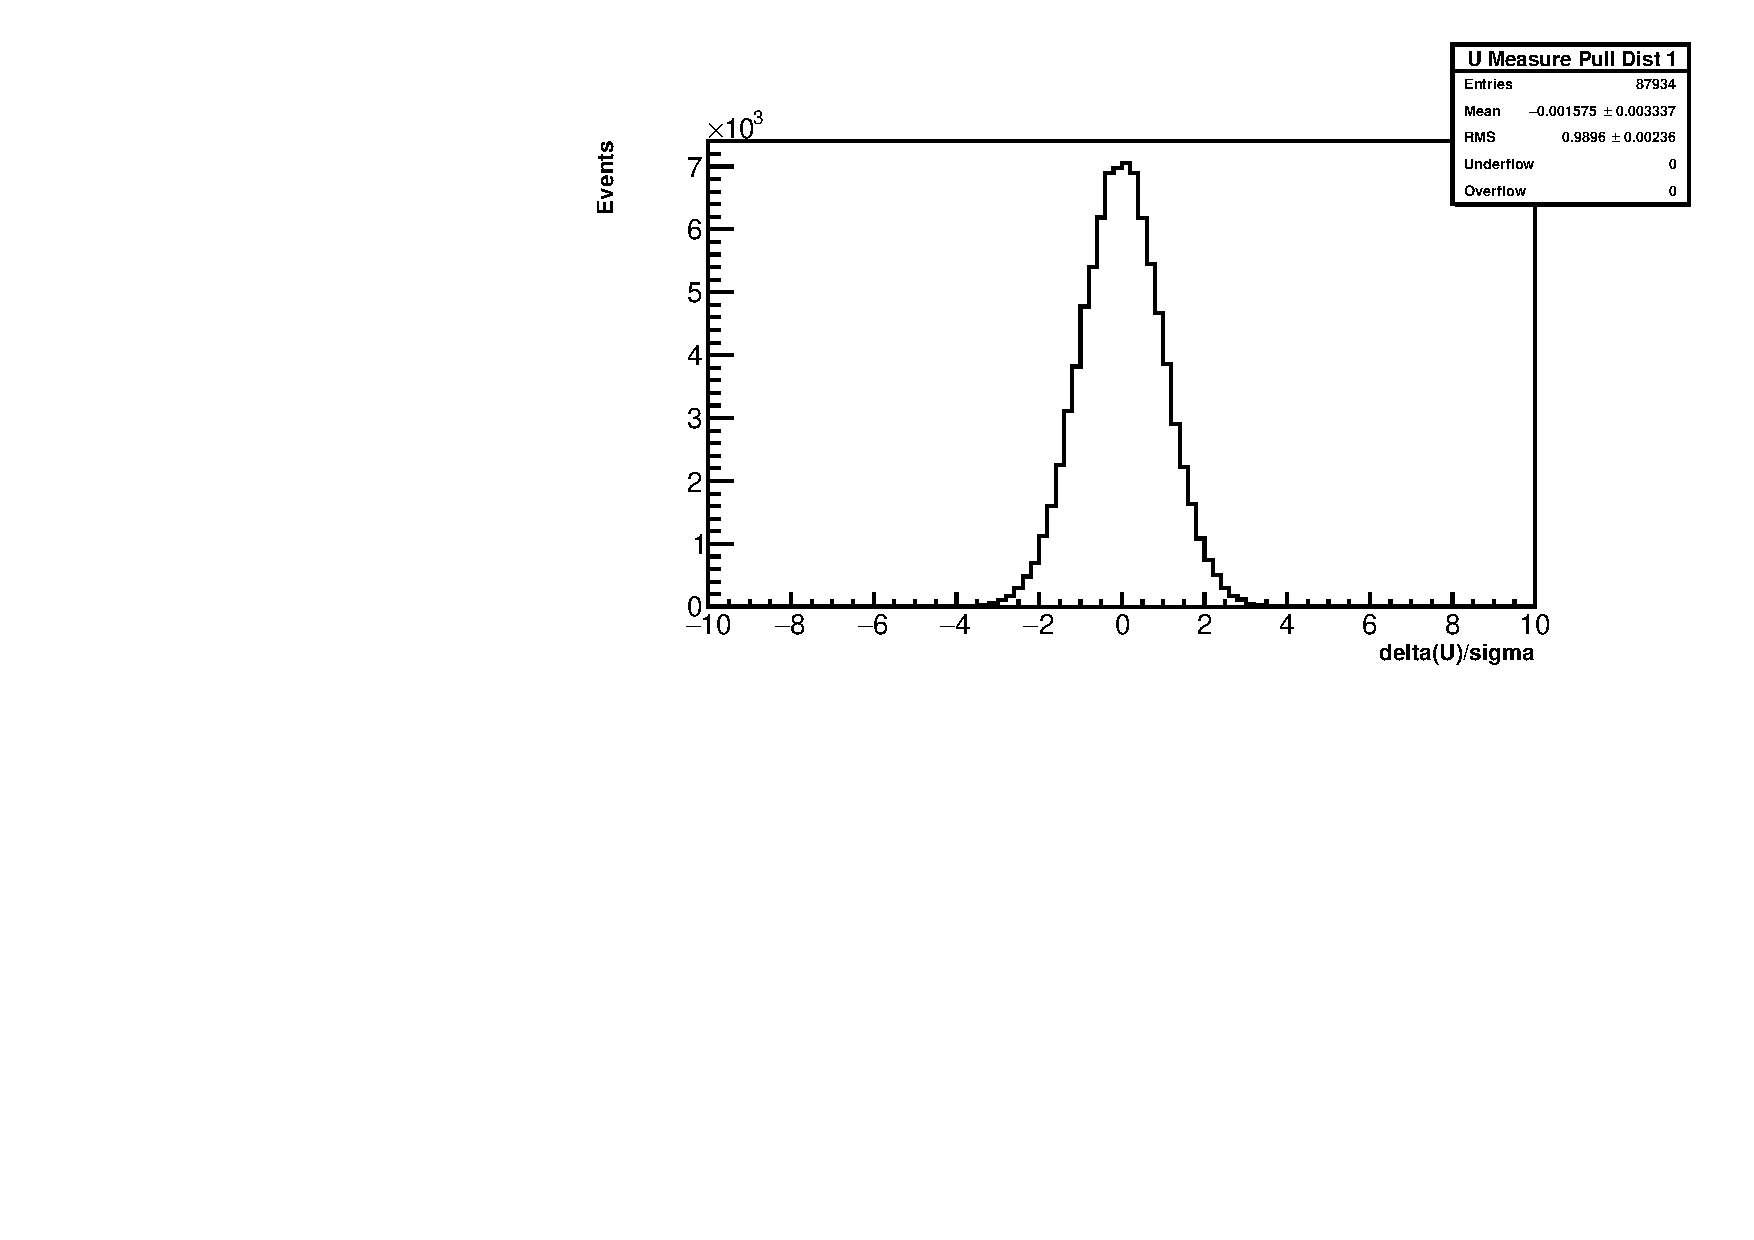
\includegraphics[width=1\textwidth]{UmeasPull} 
        \caption{U measurement pull on plane 1 as given by Equation \ref{eq:measpullmaterial}. It is a unit Gaussian within errors.}
    \end{subfigure}
    
    \begin{subfigure}[]{0.65\textwidth}
        \centering
        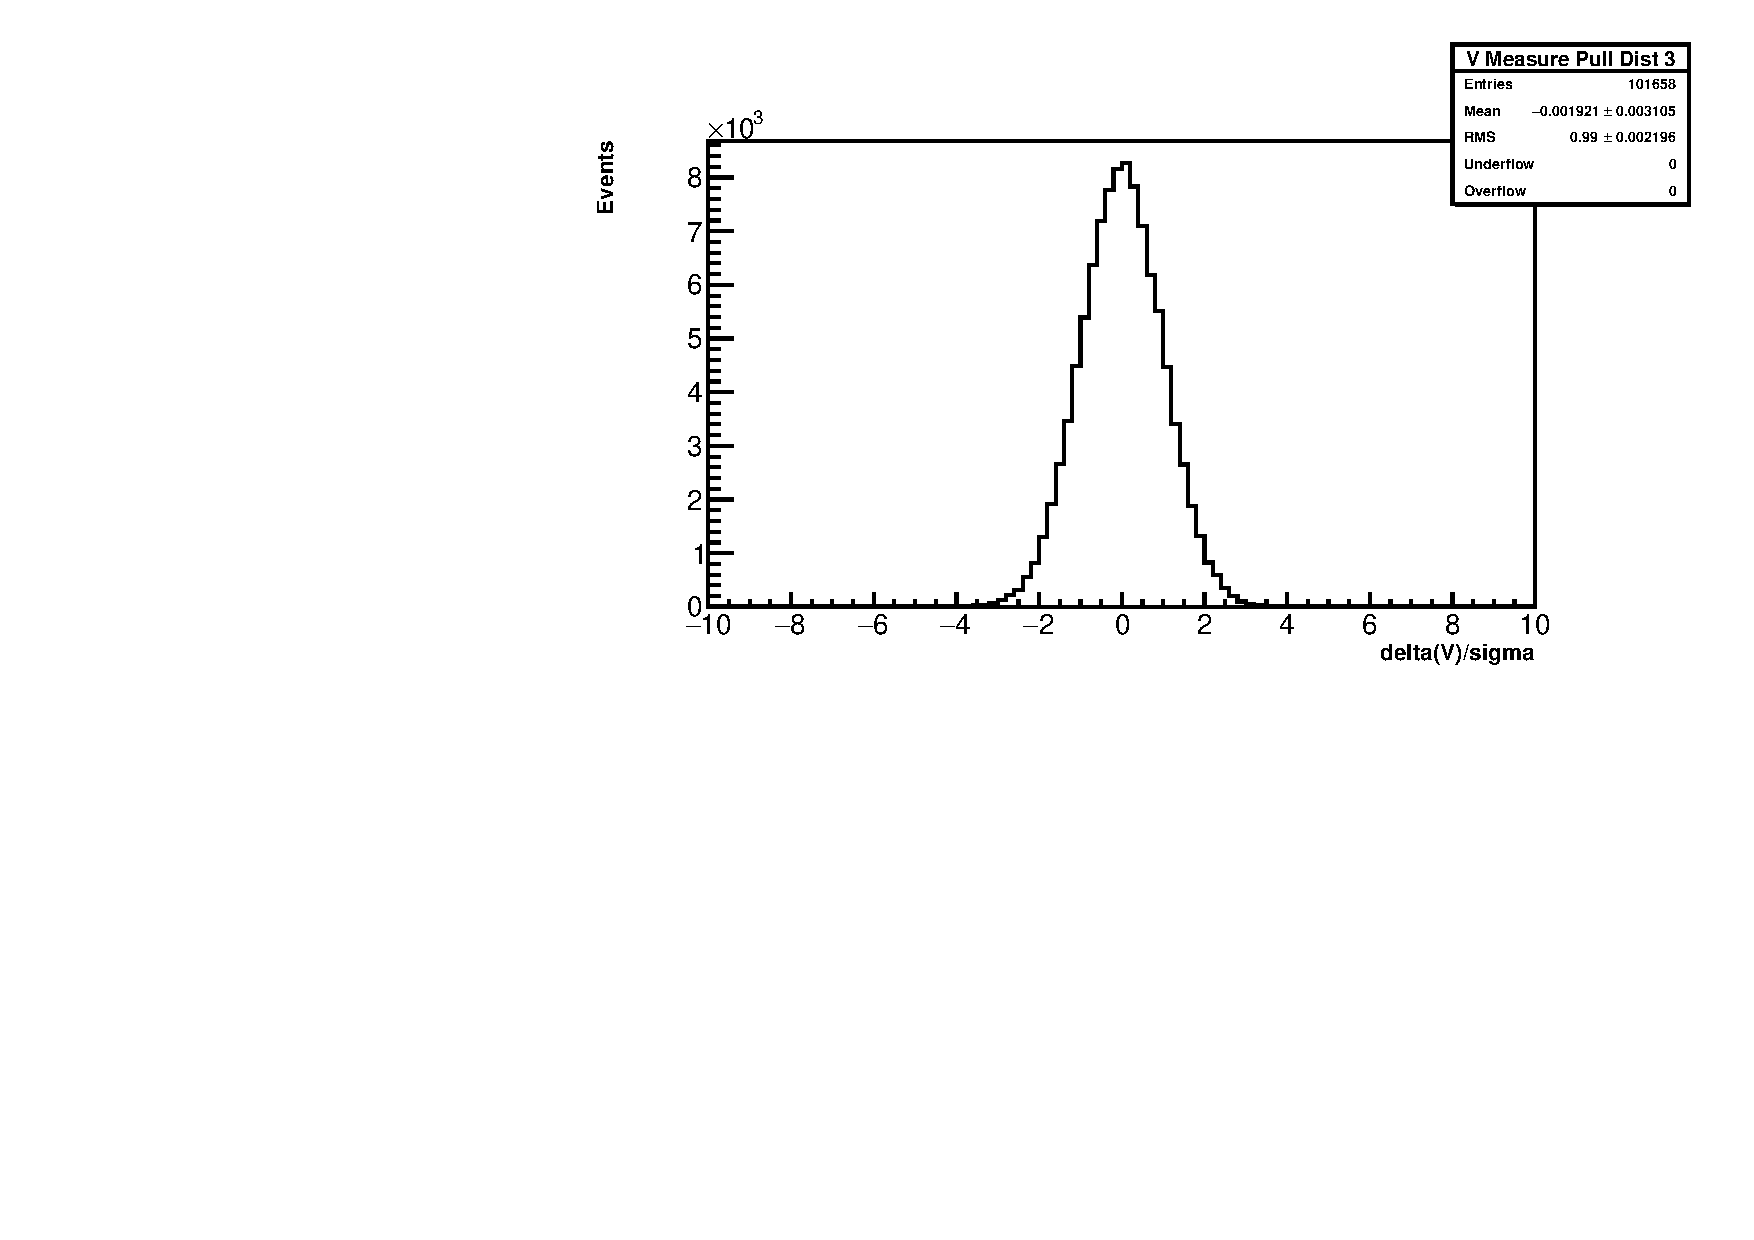
\includegraphics[width=1\textwidth]{VmeasPull} 
        \caption{V measurement pull on plane 3 as given by Equation \ref{eq:measpullmaterial}. It is a unit Gaussian within errors.}
    \end{subfigure}

    \begin{subfigure}[]{0.65\textwidth}
        \centering
        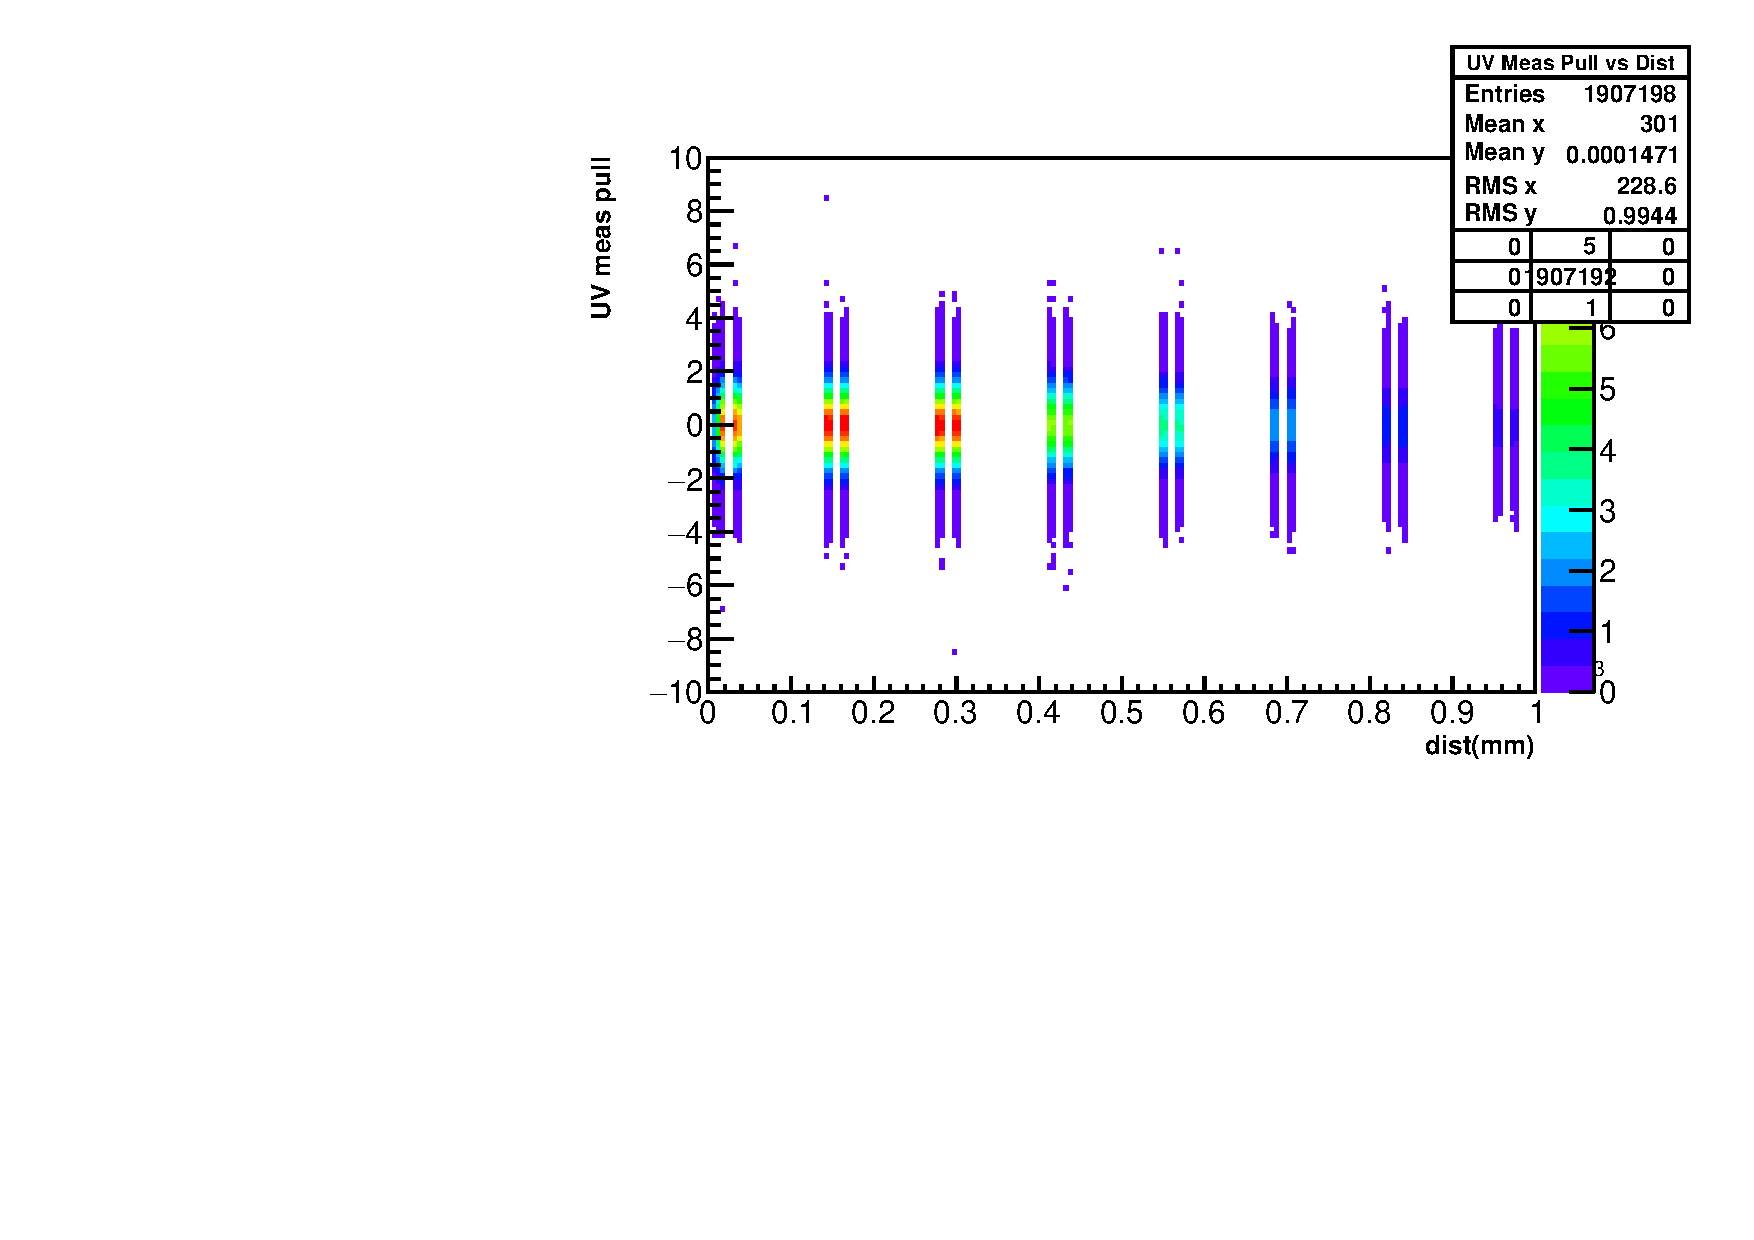
\includegraphics[width=1\textwidth]{UVMeasPullVsDist} 
        \caption{U and V measurement pulls as a function of track distance from fitting start point, or ``0'' plane. The RMS drops slightly as a function of distance, indicated imperfectly attuned errors.}
    \end{subfigure}

    \caption{Measurement pull plots, useful for track fitting on data validation.}
\end{figure}



\begin{figure}
    \centering
    \begin{subfigure}[]{0.65\textwidth}
        \centering
        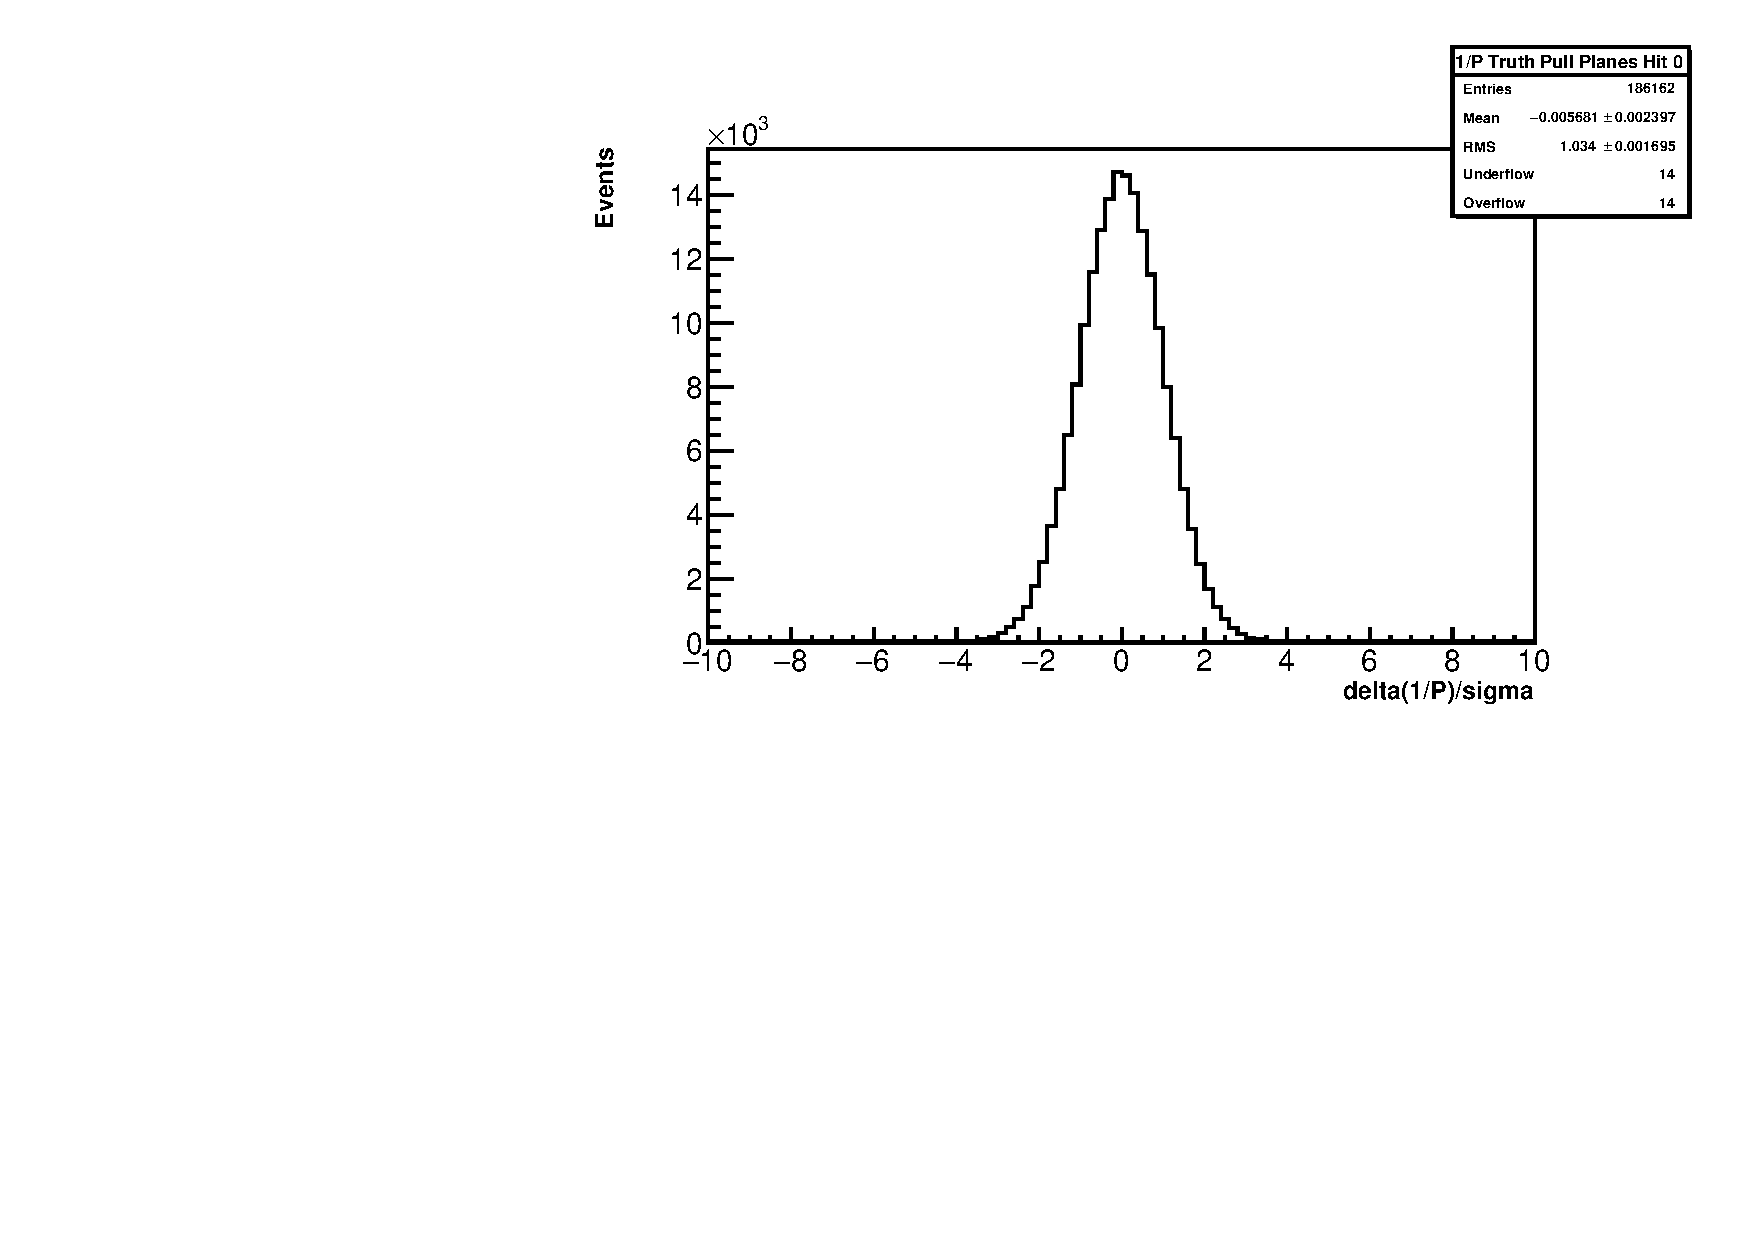
\includegraphics[width=1\textwidth]{1Ppull} 
        \caption{1/P truth pull on plane 0 for all tracks. Very close to a unit Gaussian showing the tracking is working correctly.}
    \end{subfigure}
    
    \begin{subfigure}[]{0.65\textwidth}
        \centering
        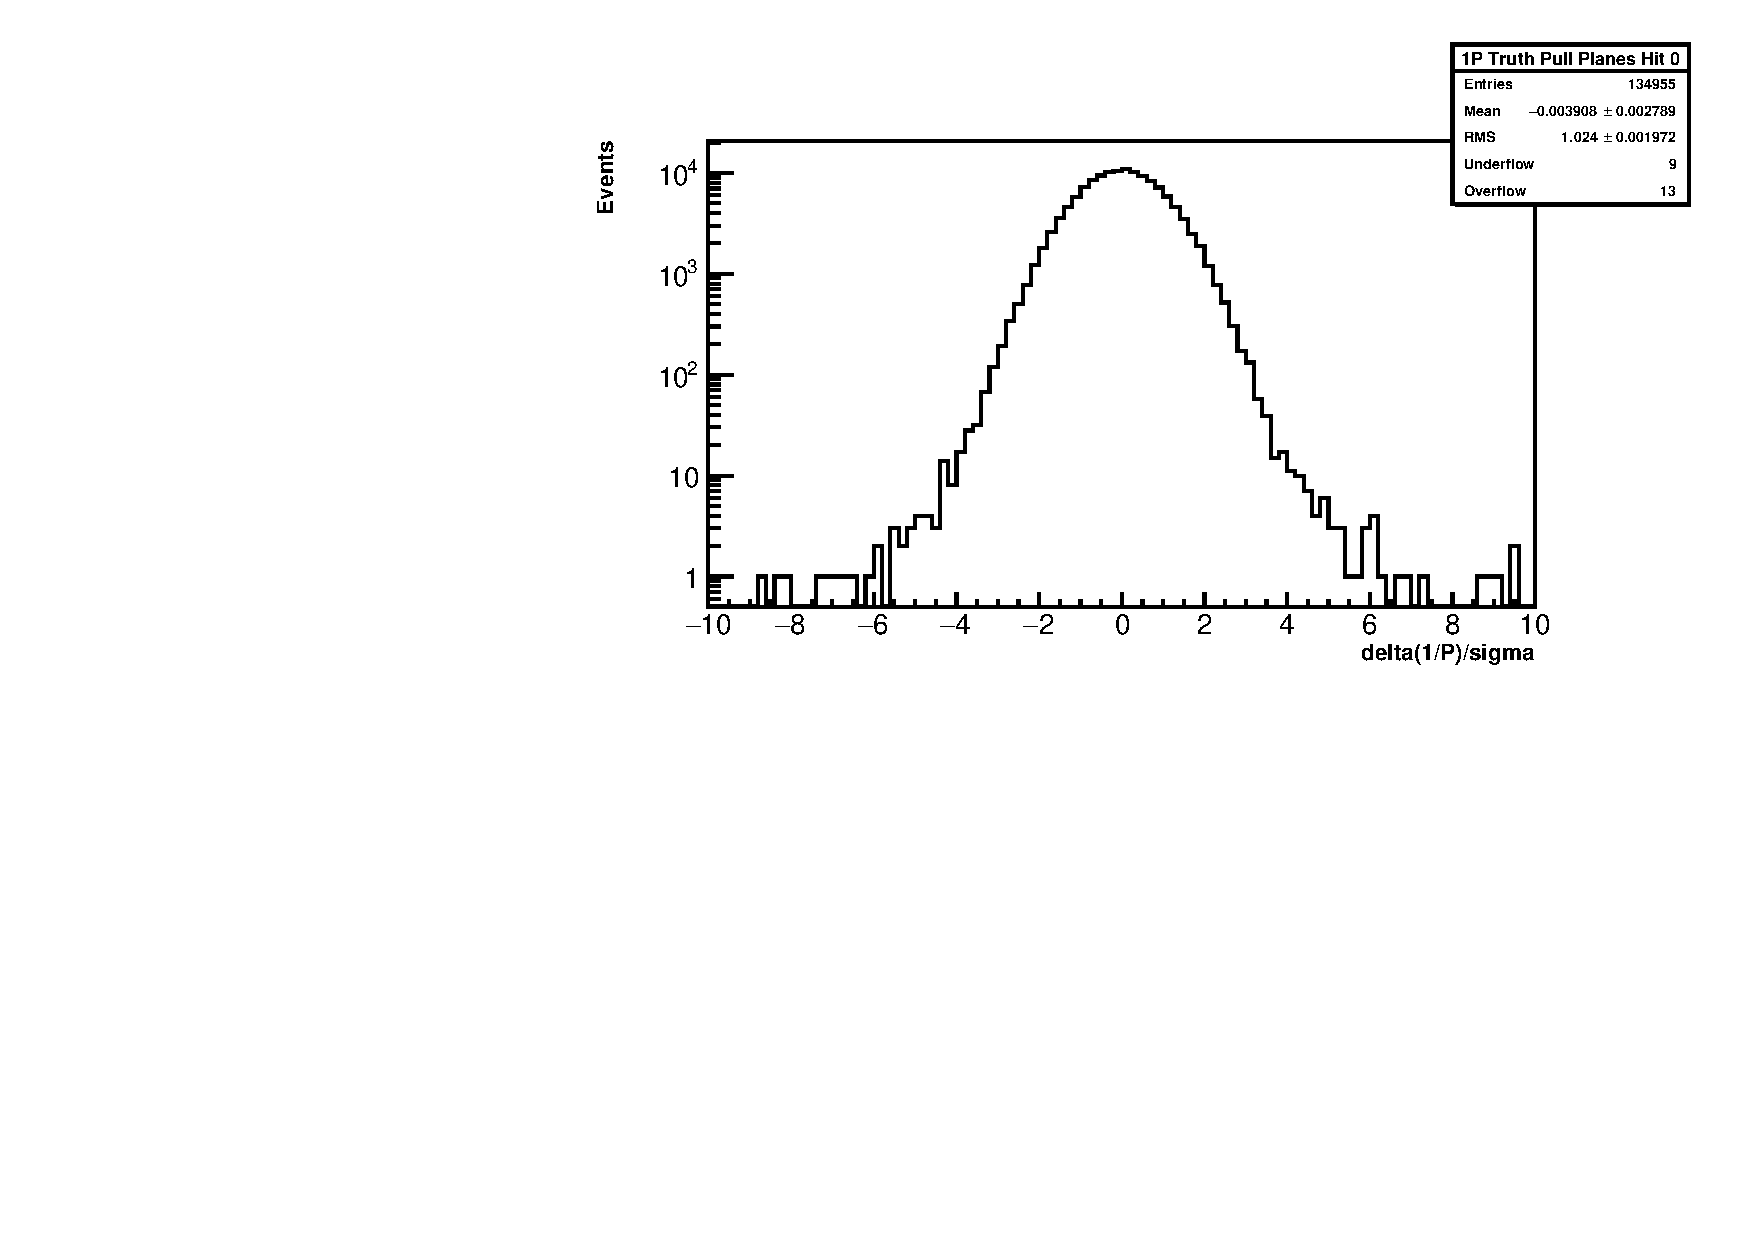
\includegraphics[width=1\textwidth]{1PpullLog} 
        \caption{1/P truth pull on plane 0 for all tracks, log plot. Poor events can be seen as the distribution spreads out more towards the edges, with some under and overflows.}
    \end{subfigure}

    \begin{subfigure}[]{0.65\textwidth}
        \centering
        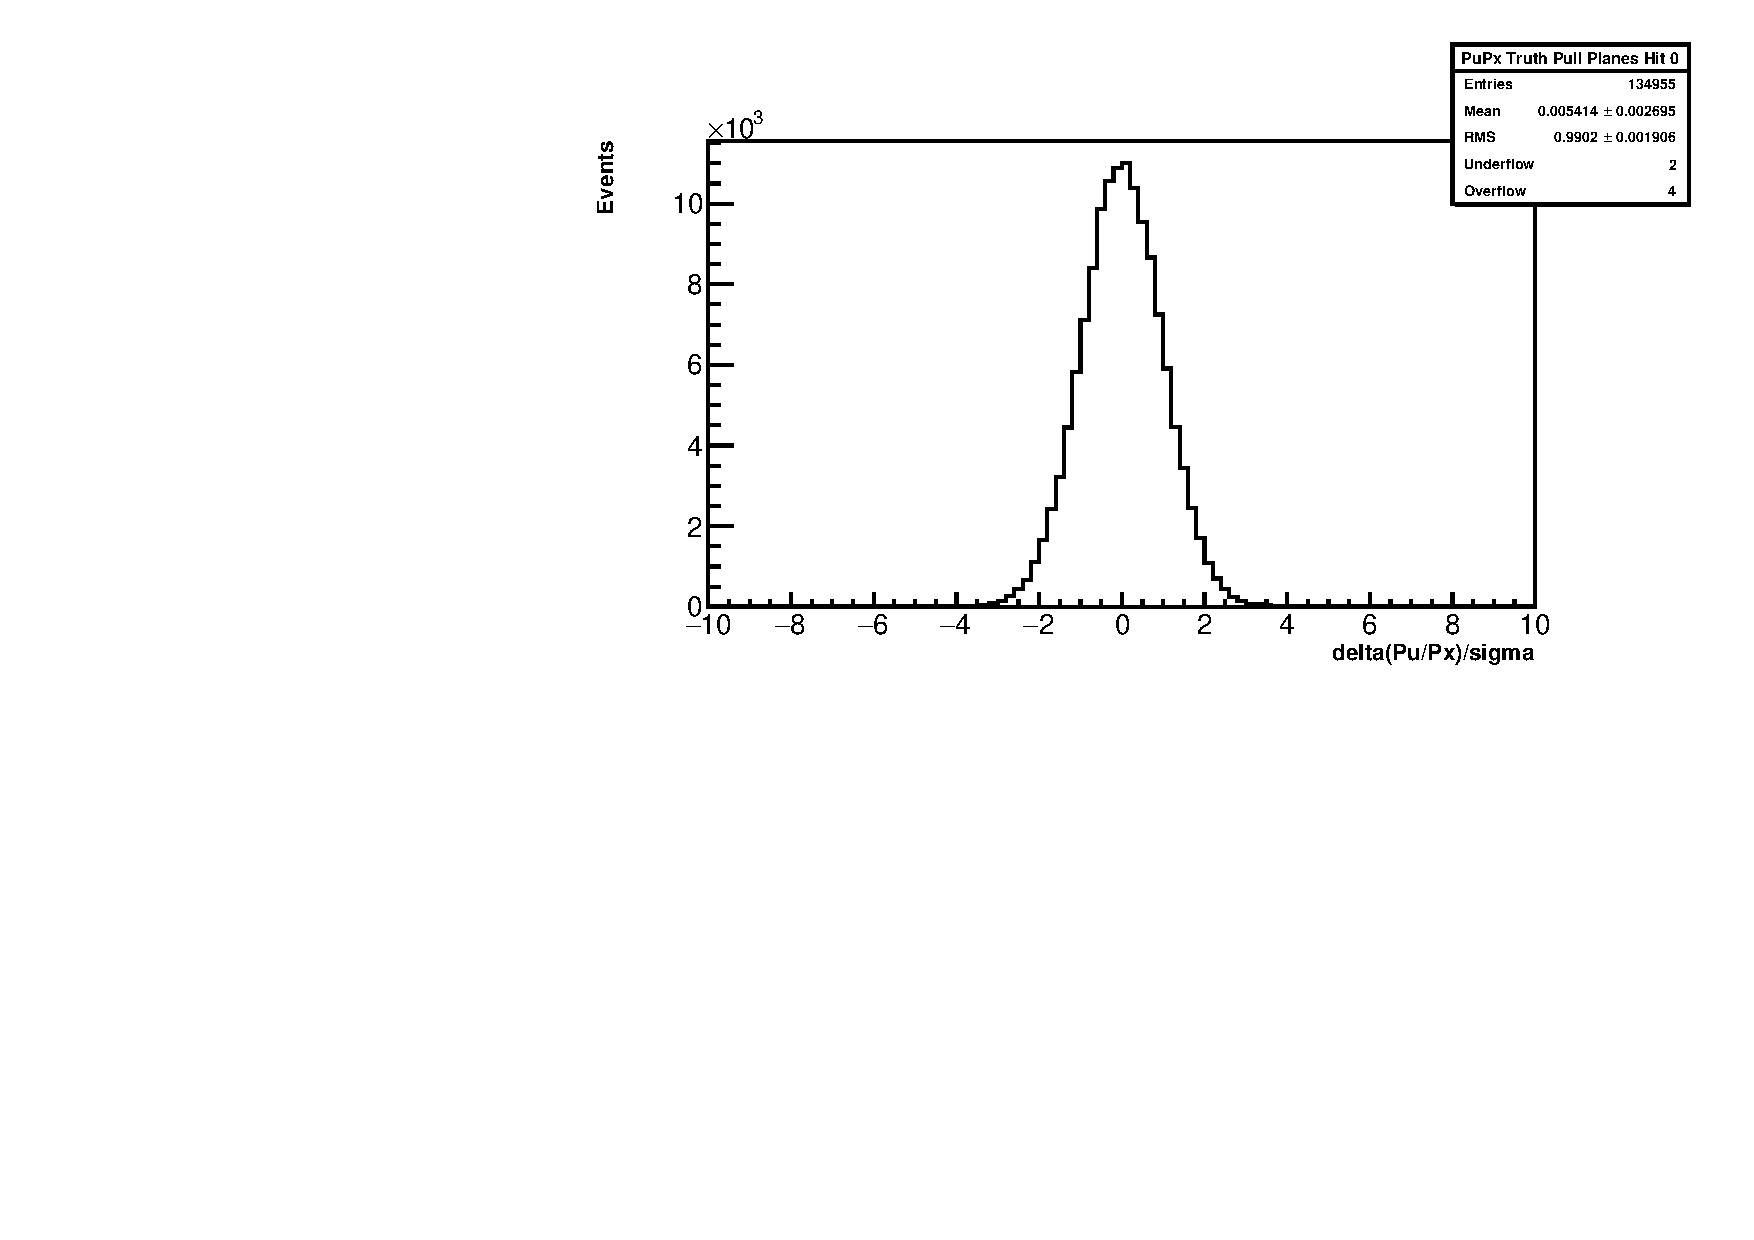
\includegraphics[width=1\textwidth]{PuPxpull} 
        \caption{Pu/Px truth pull on plane 0 for all tracks. Very close to a unit Gaussian showing the tracking is working correctly.}
    \end{subfigure}

    \caption{Truth pulls on plane 0 for all tracks.}
\end{figure}



\begin{figure}
    \centering
    \begin{subfigure}[]{0.65\textwidth}
        \centering
        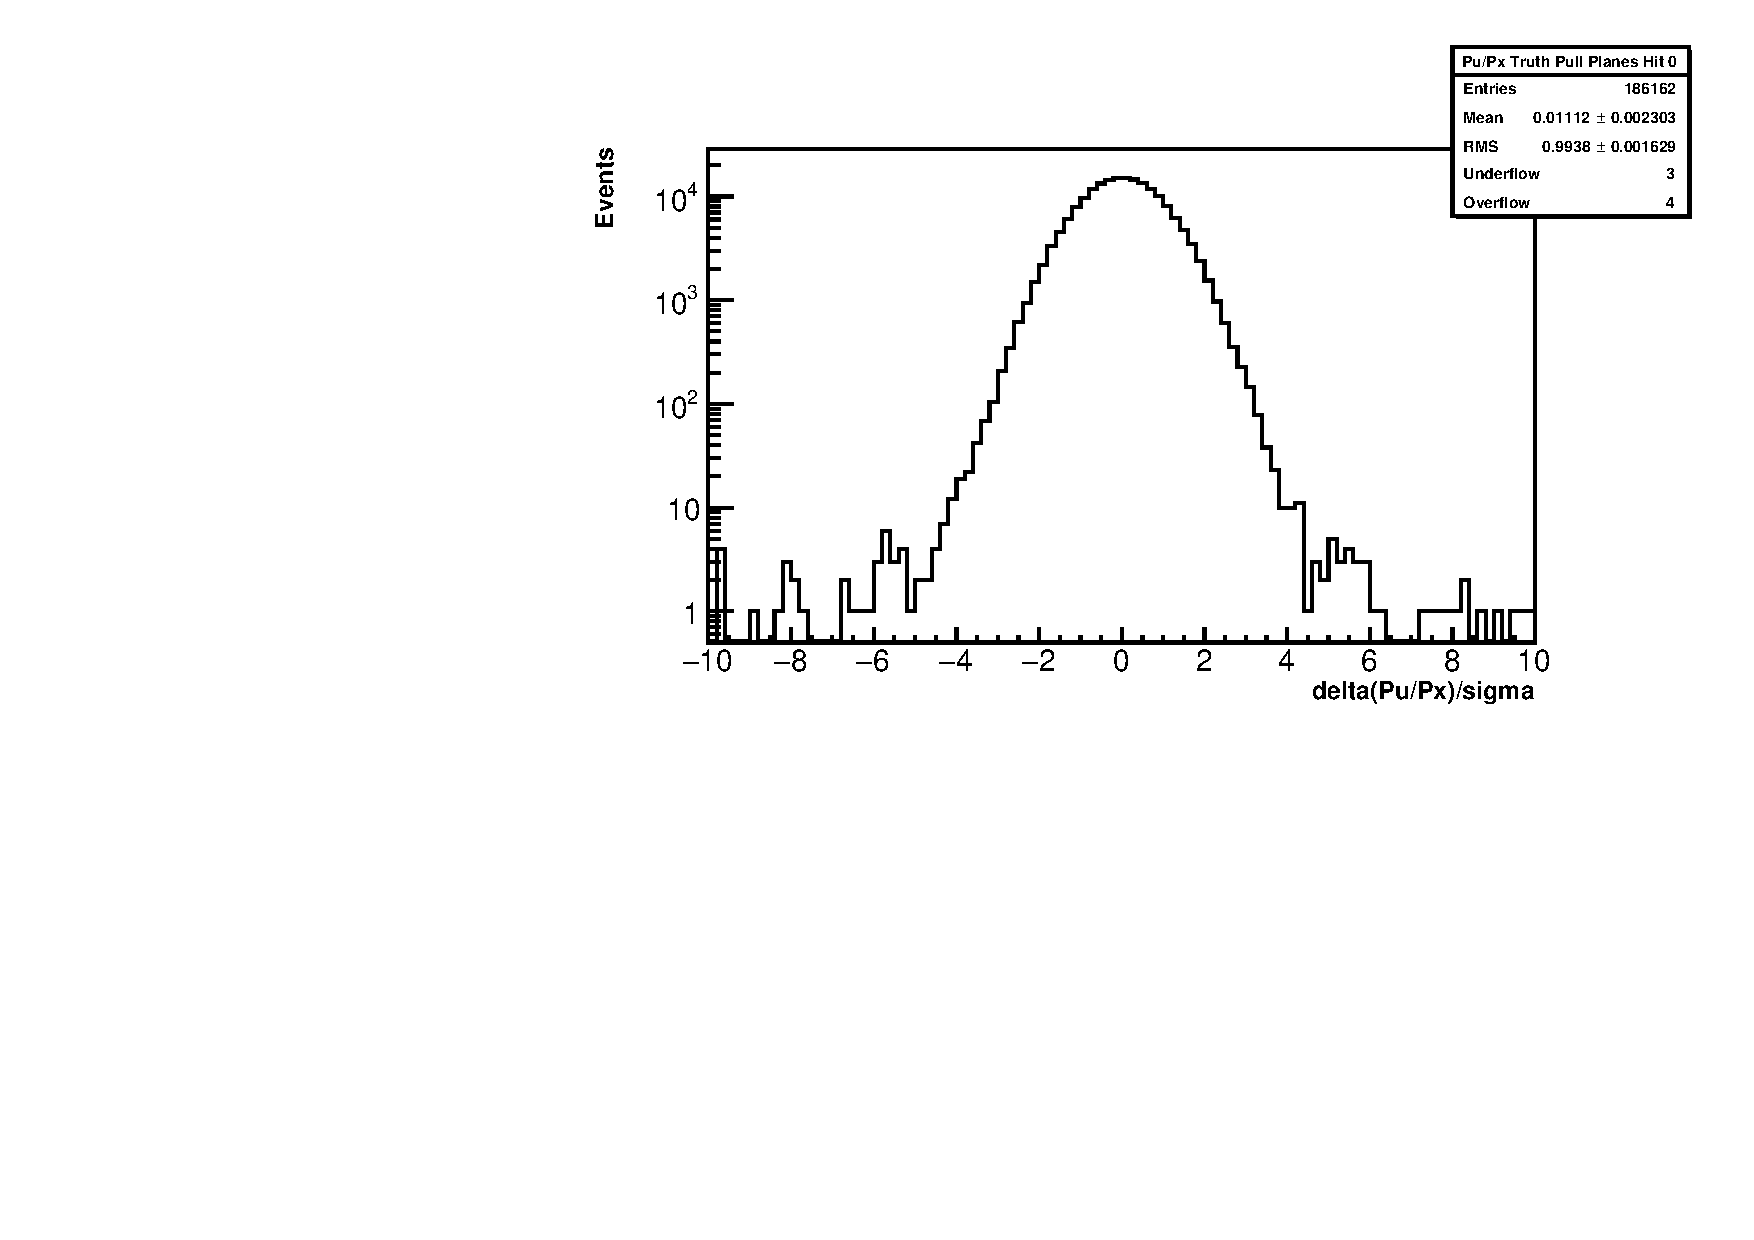
\includegraphics[width=1\textwidth]{PuPxpullLog} 
        \caption{Pu/Px truth pull on plane 0 for all tracks, log plot. Poor events can be seen as the distribution spreads out more towards the edges, with some under and overflows.}
    \end{subfigure}
    
    \begin{subfigure}[]{0.65\textwidth}
        \centering
        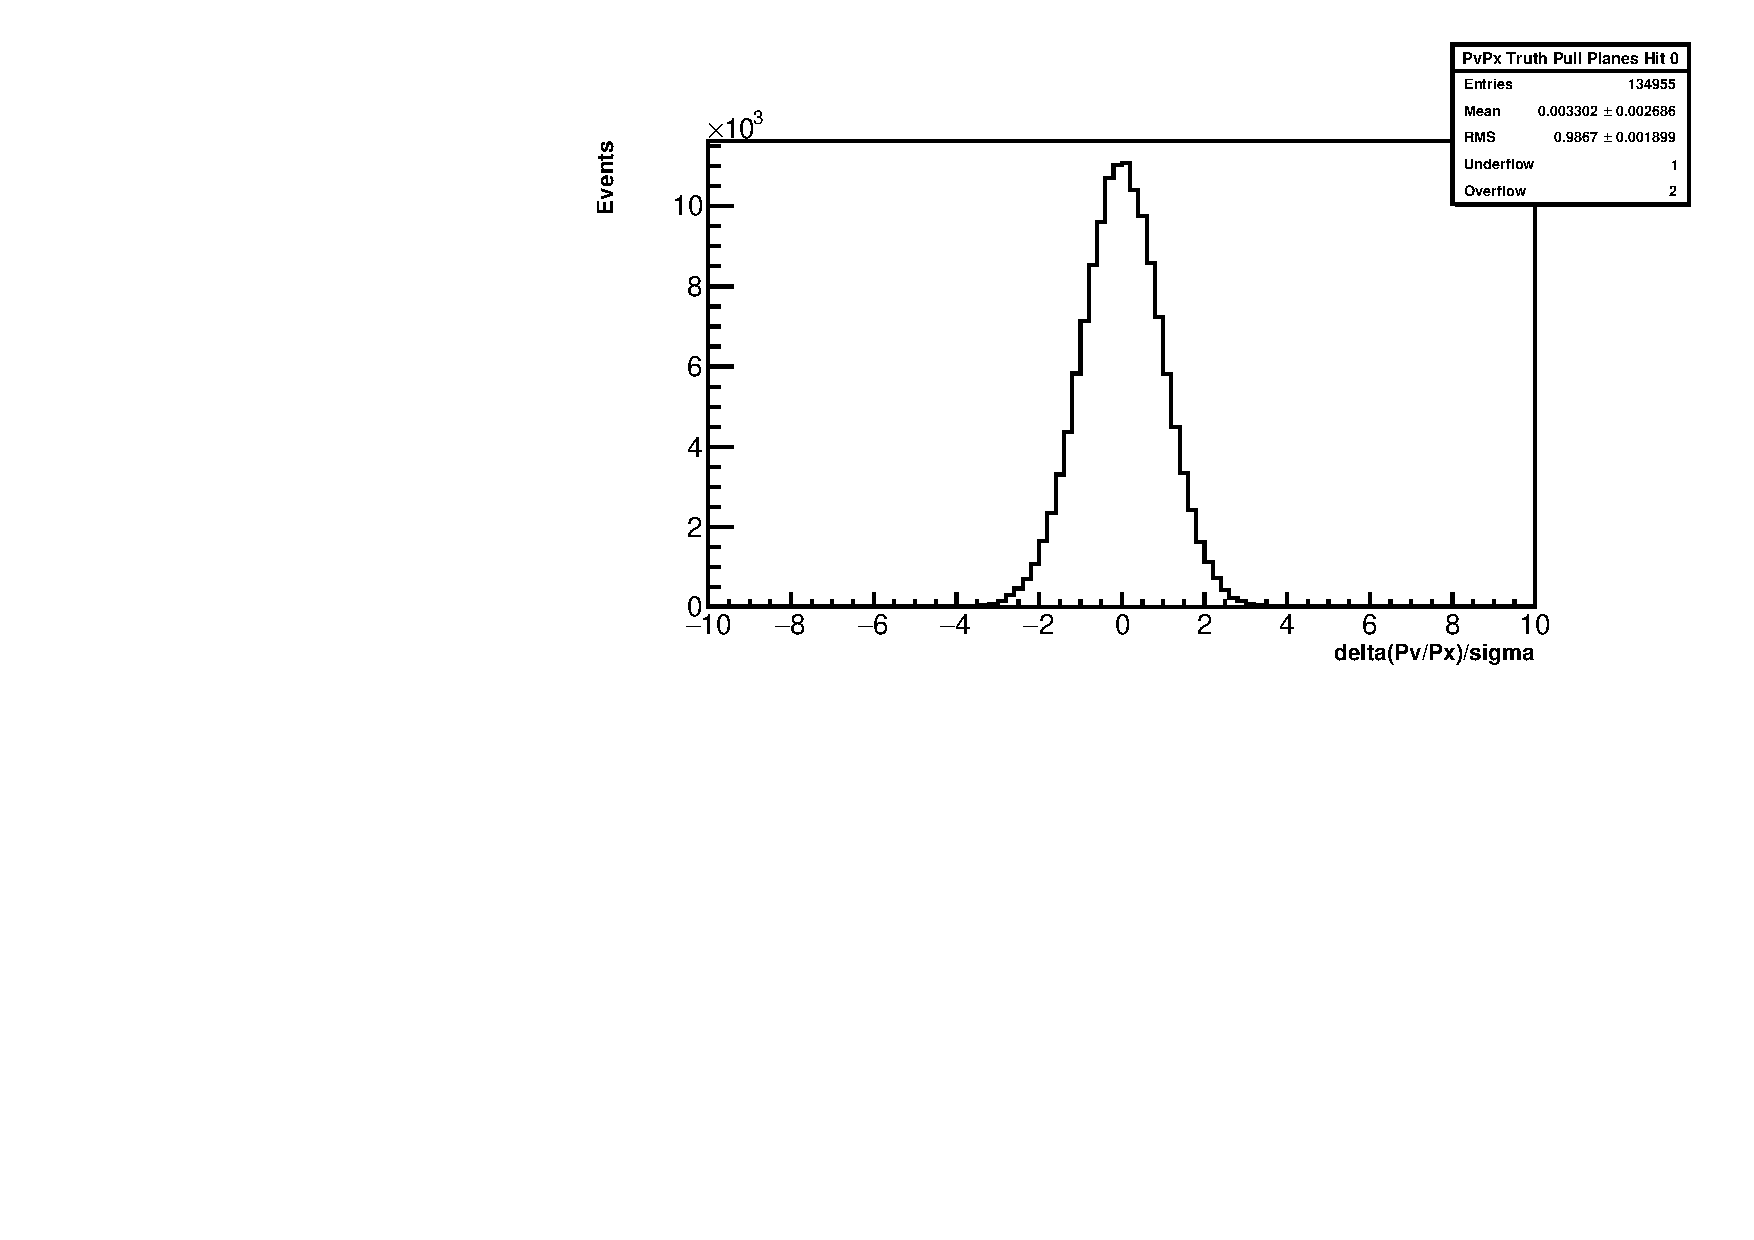
\includegraphics[width=1\textwidth]{PvPxpull} 
        \caption{Pv/Px truth pull on plane 0 for all tracks. Very close to a unit Gaussian showing the tracking is working correctly.}
    \end{subfigure}

    \begin{subfigure}[]{0.65\textwidth}
        \centering
        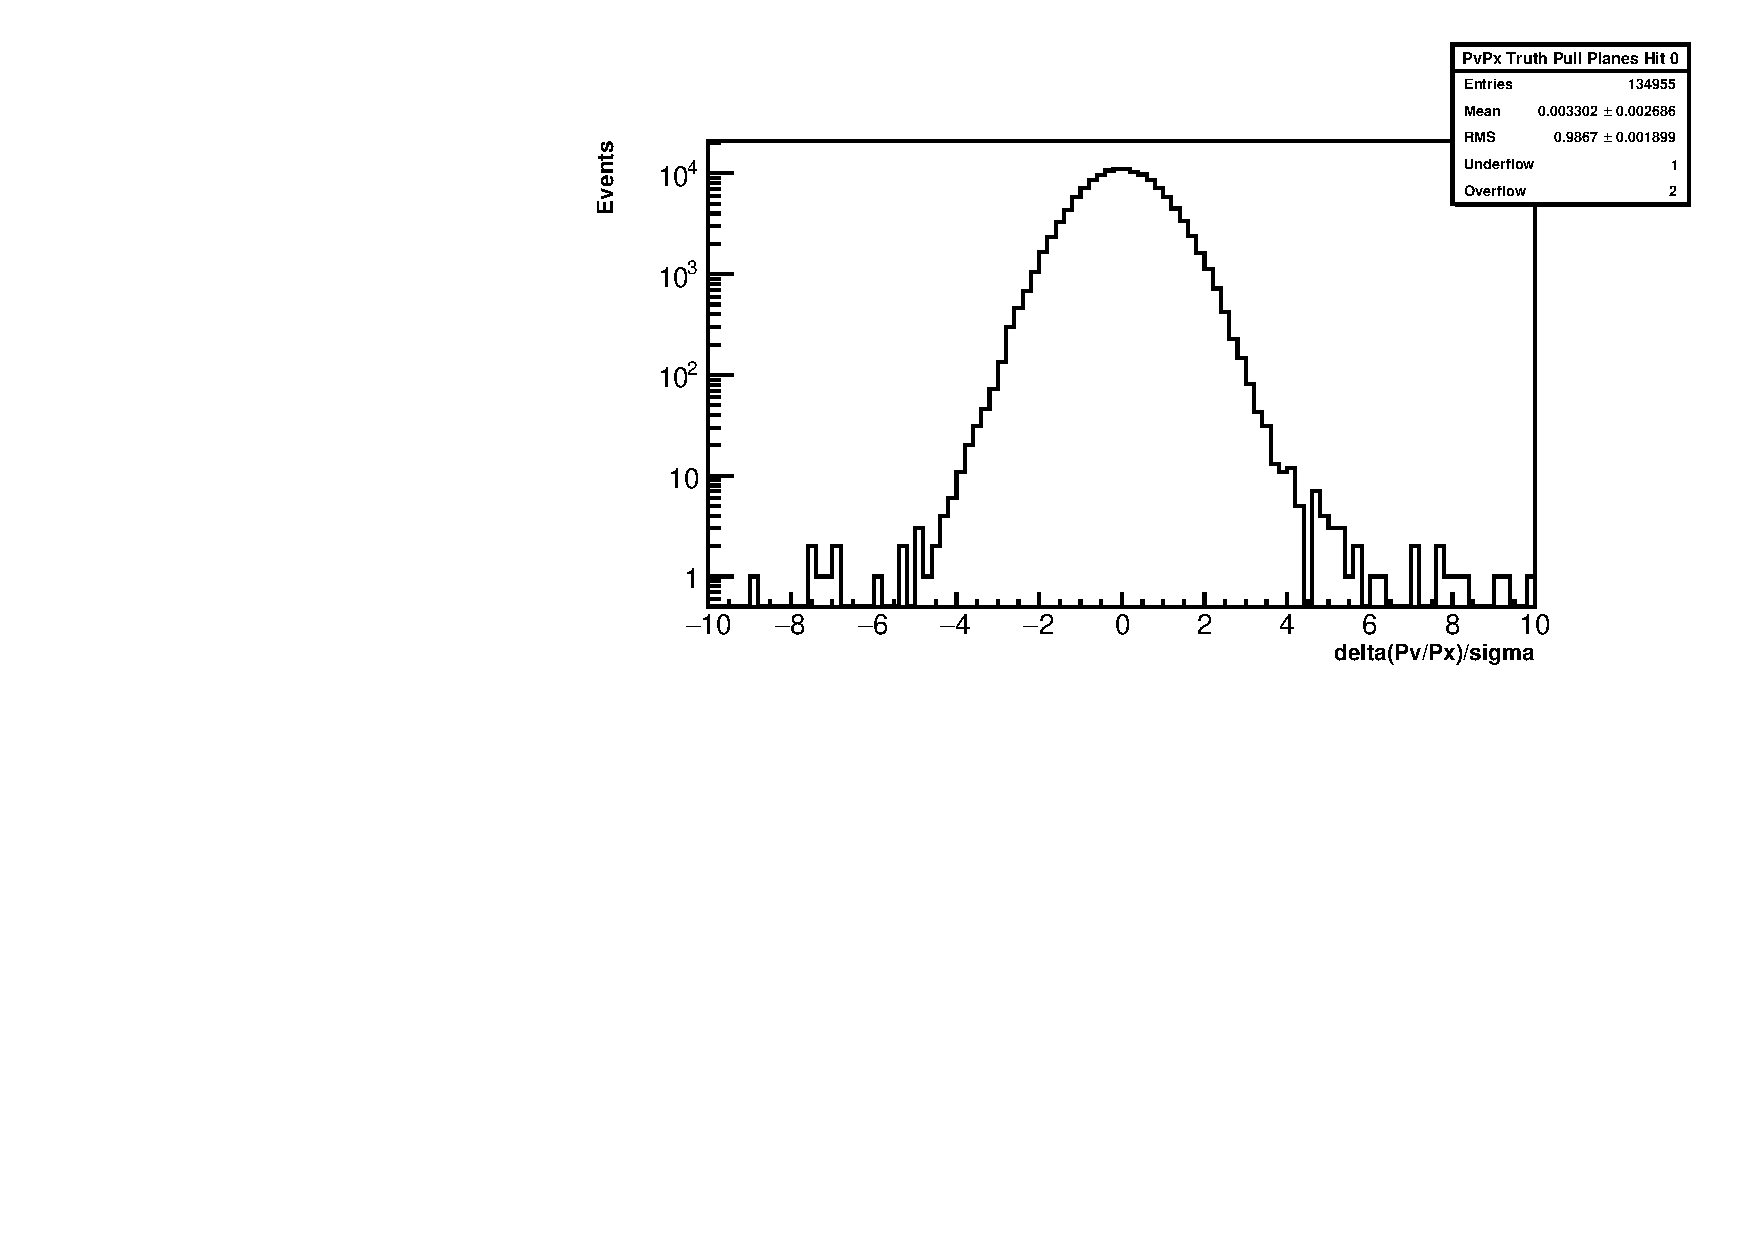
\includegraphics[width=1\textwidth]{PvPxpullLog} 
        \caption{Pv/Px truth pull on plane 0 for all tracks, log plot. Poor events can be seen as the distribution spreads out more towards the edges, with some under and overflows.}
    \end{subfigure}

    \caption{Truth pulls on plane 0 for all tracks.}
\end{figure}



\begin{figure}
    \centering
    \begin{subfigure}[]{0.8\textwidth}
        \centering
        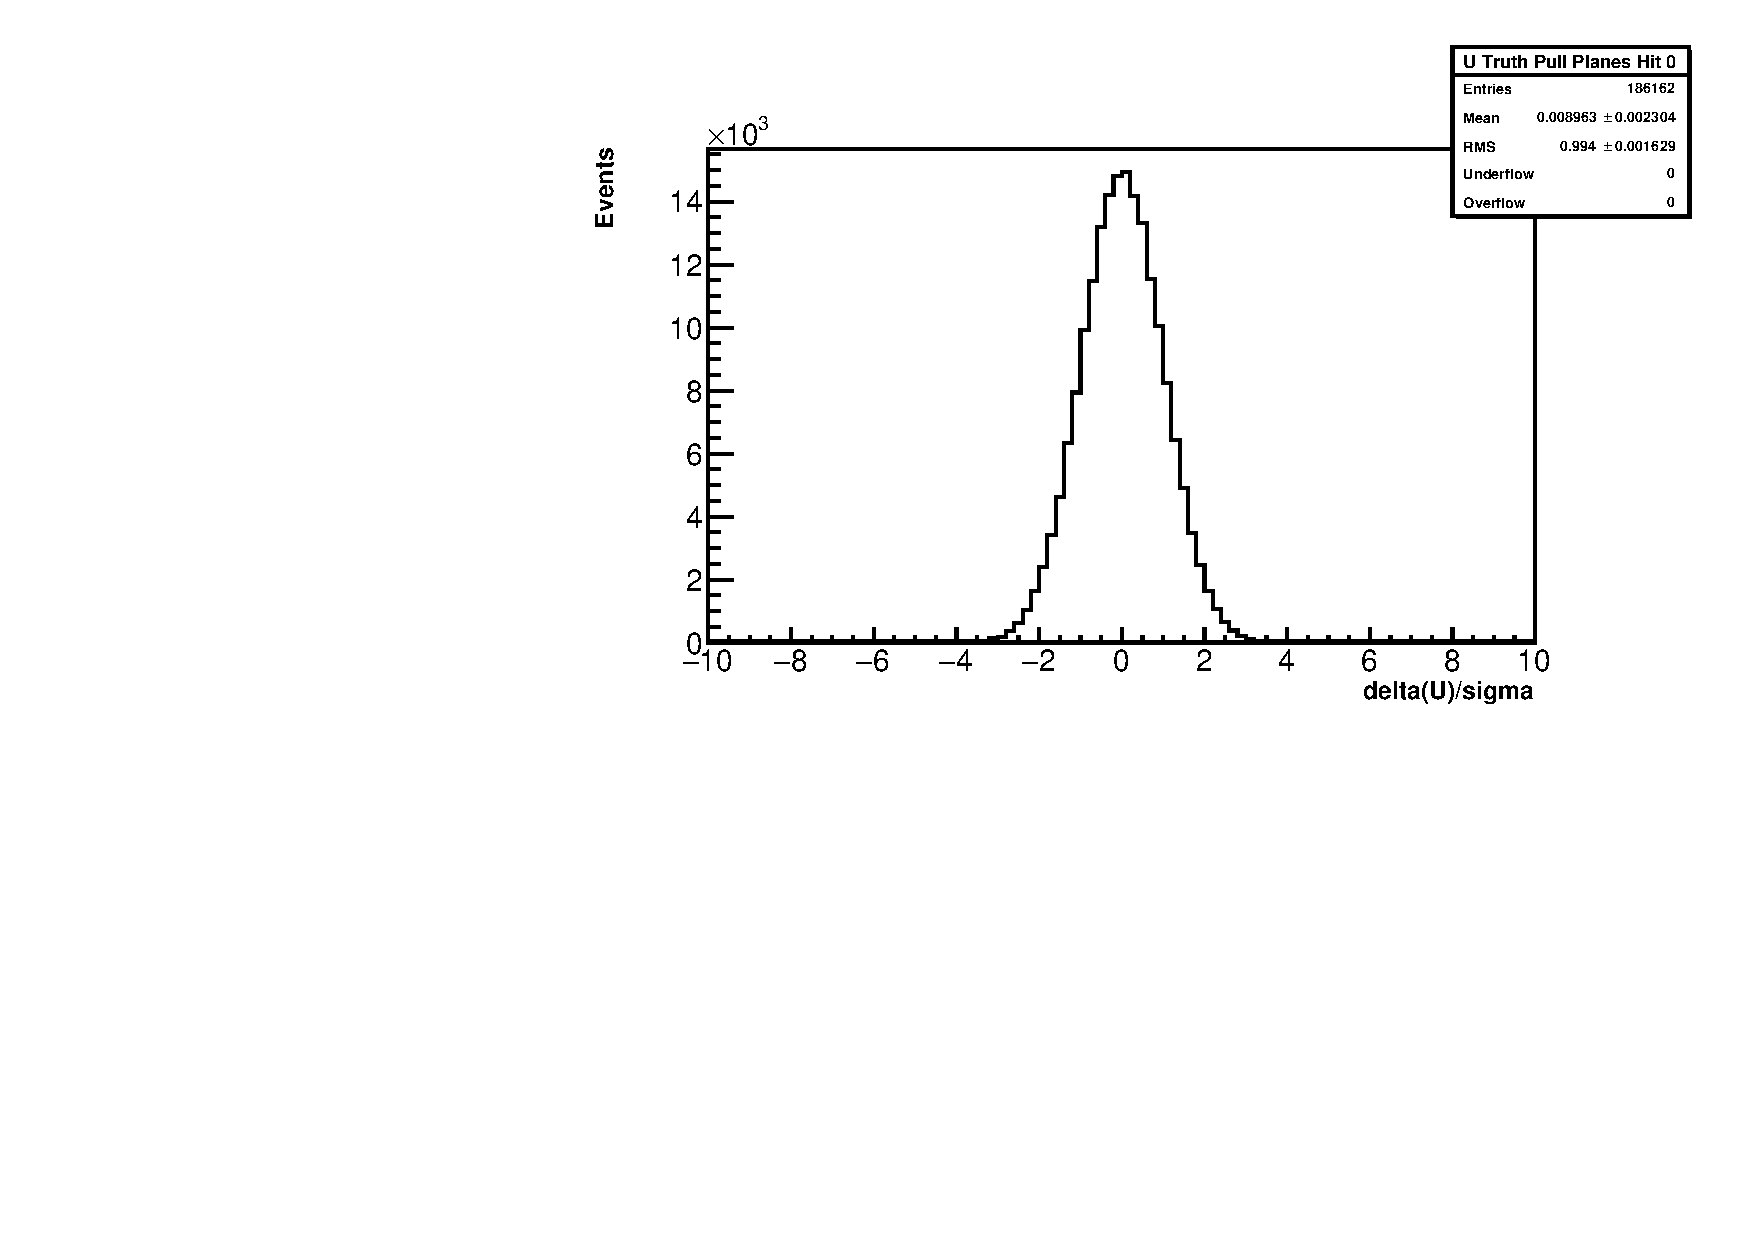
\includegraphics[width=1\textwidth]{Upull} 
        \caption{U truth pull on plane 0 for all tracks. Very close to a unit Gaussian showing the tracking is working correctly.}
    \end{subfigure}
    
    \begin{subfigure}[]{0.8\textwidth}
        \centering
        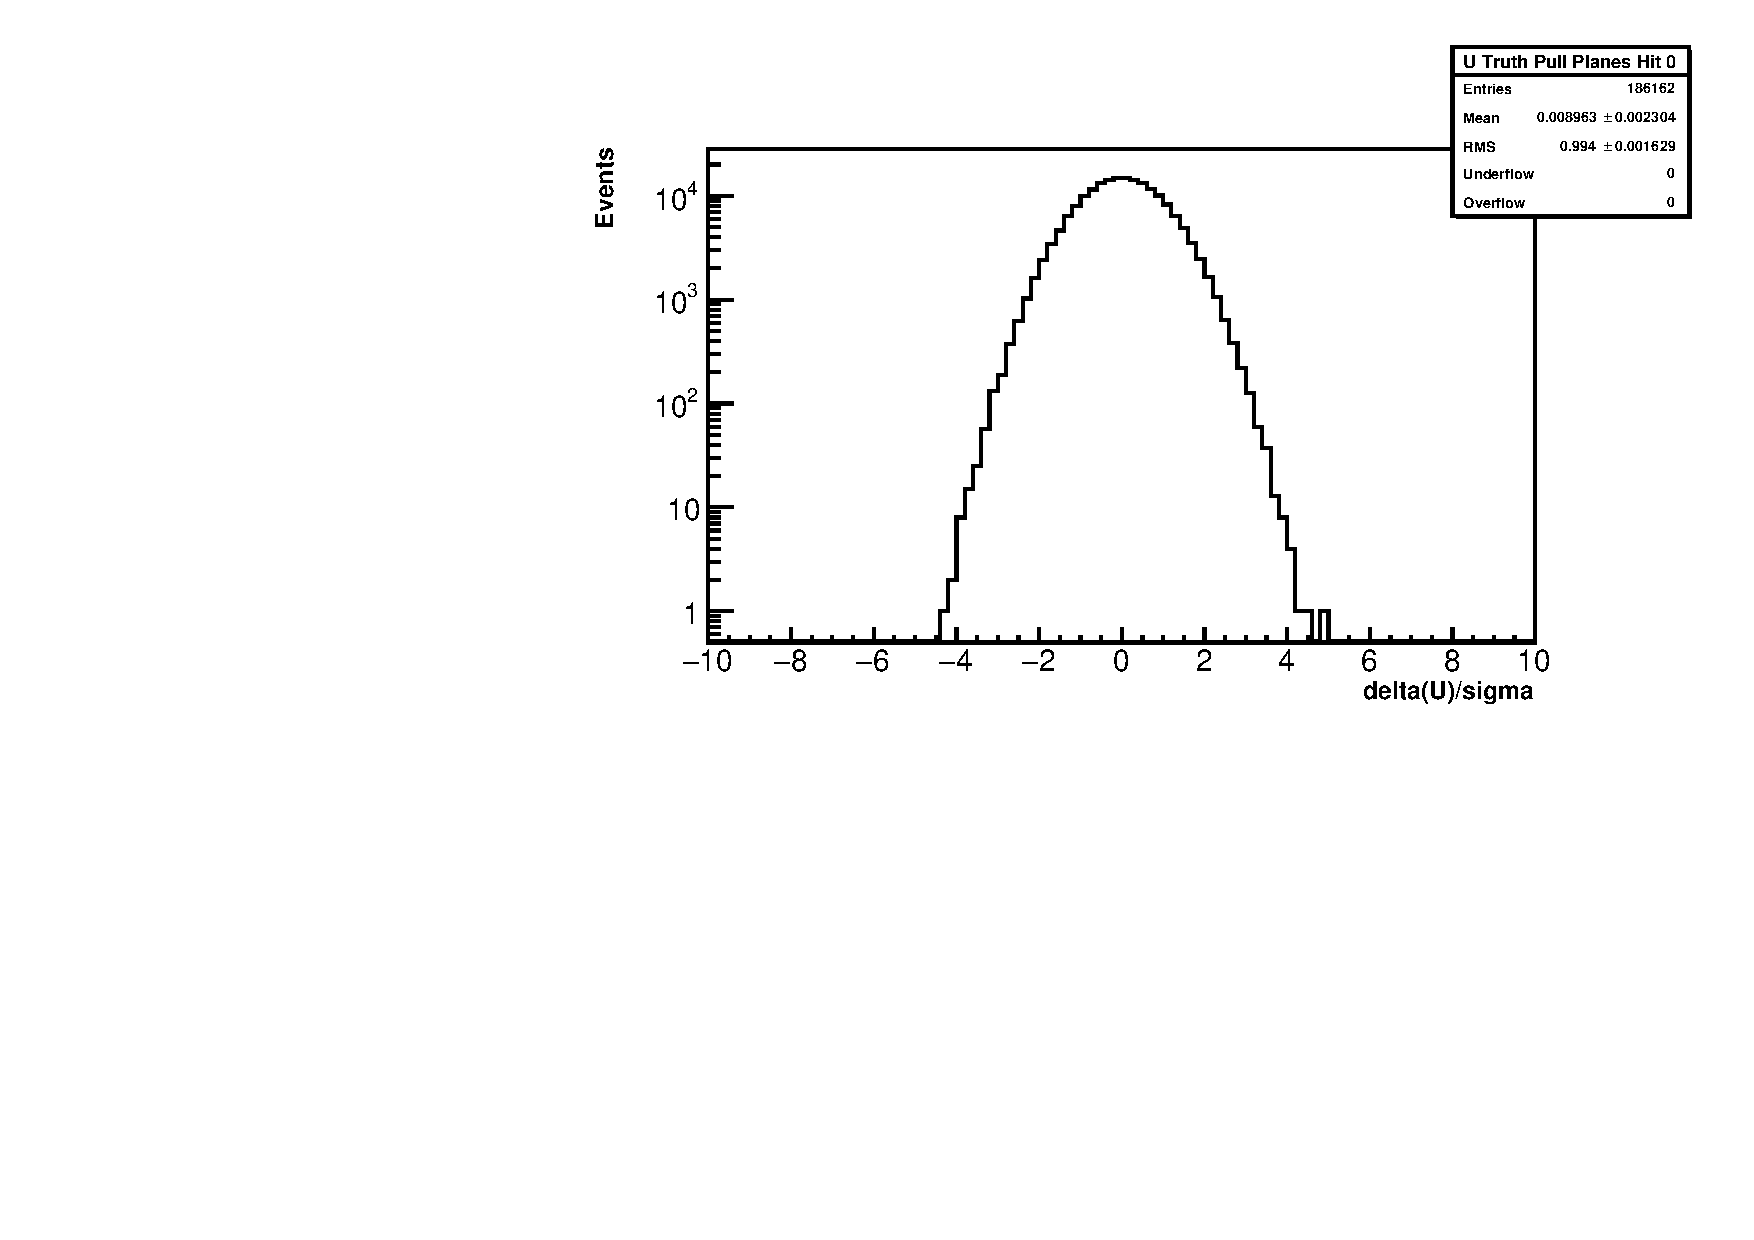
\includegraphics[width=1\textwidth]{UpullLog} 
        \caption{U truth pull on plane 0 for all tracks, log plot. Poor events can be seen as the distribution spreads out more towards the edges, with some under and overflows.}
    \end{subfigure}

    \caption{Number of iterations information.}
\end{figure}

\begin{figure}
    \centering
    \begin{subfigure}[]{0.8\textwidth}
        \centering
        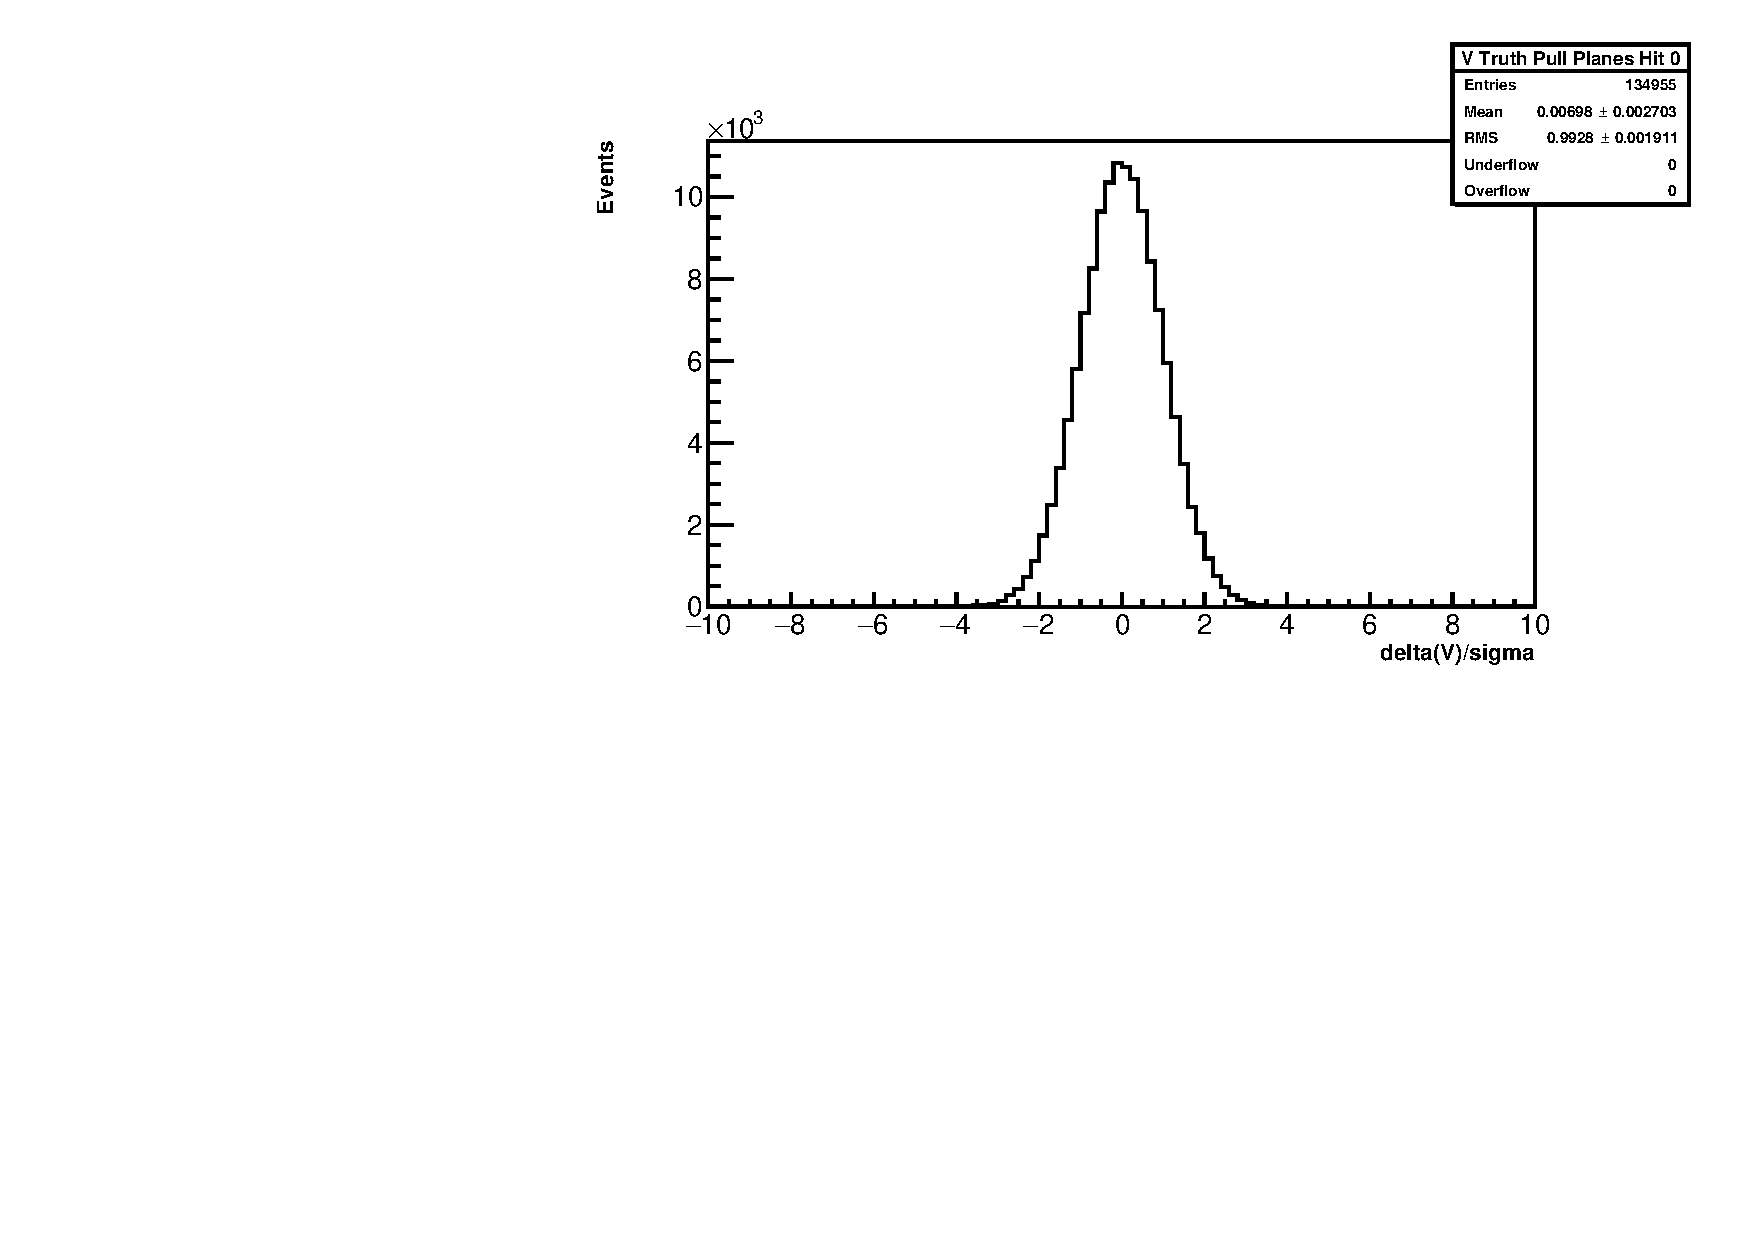
\includegraphics[width=1\textwidth]{Vpull} 
        \caption{V truth pull on plane 0 for all tracks. Very close to a unit Gaussian showing the tracking is working correctly.}
    \end{subfigure}
    
    \begin{subfigure}[]{0.8\textwidth}
        \centering
        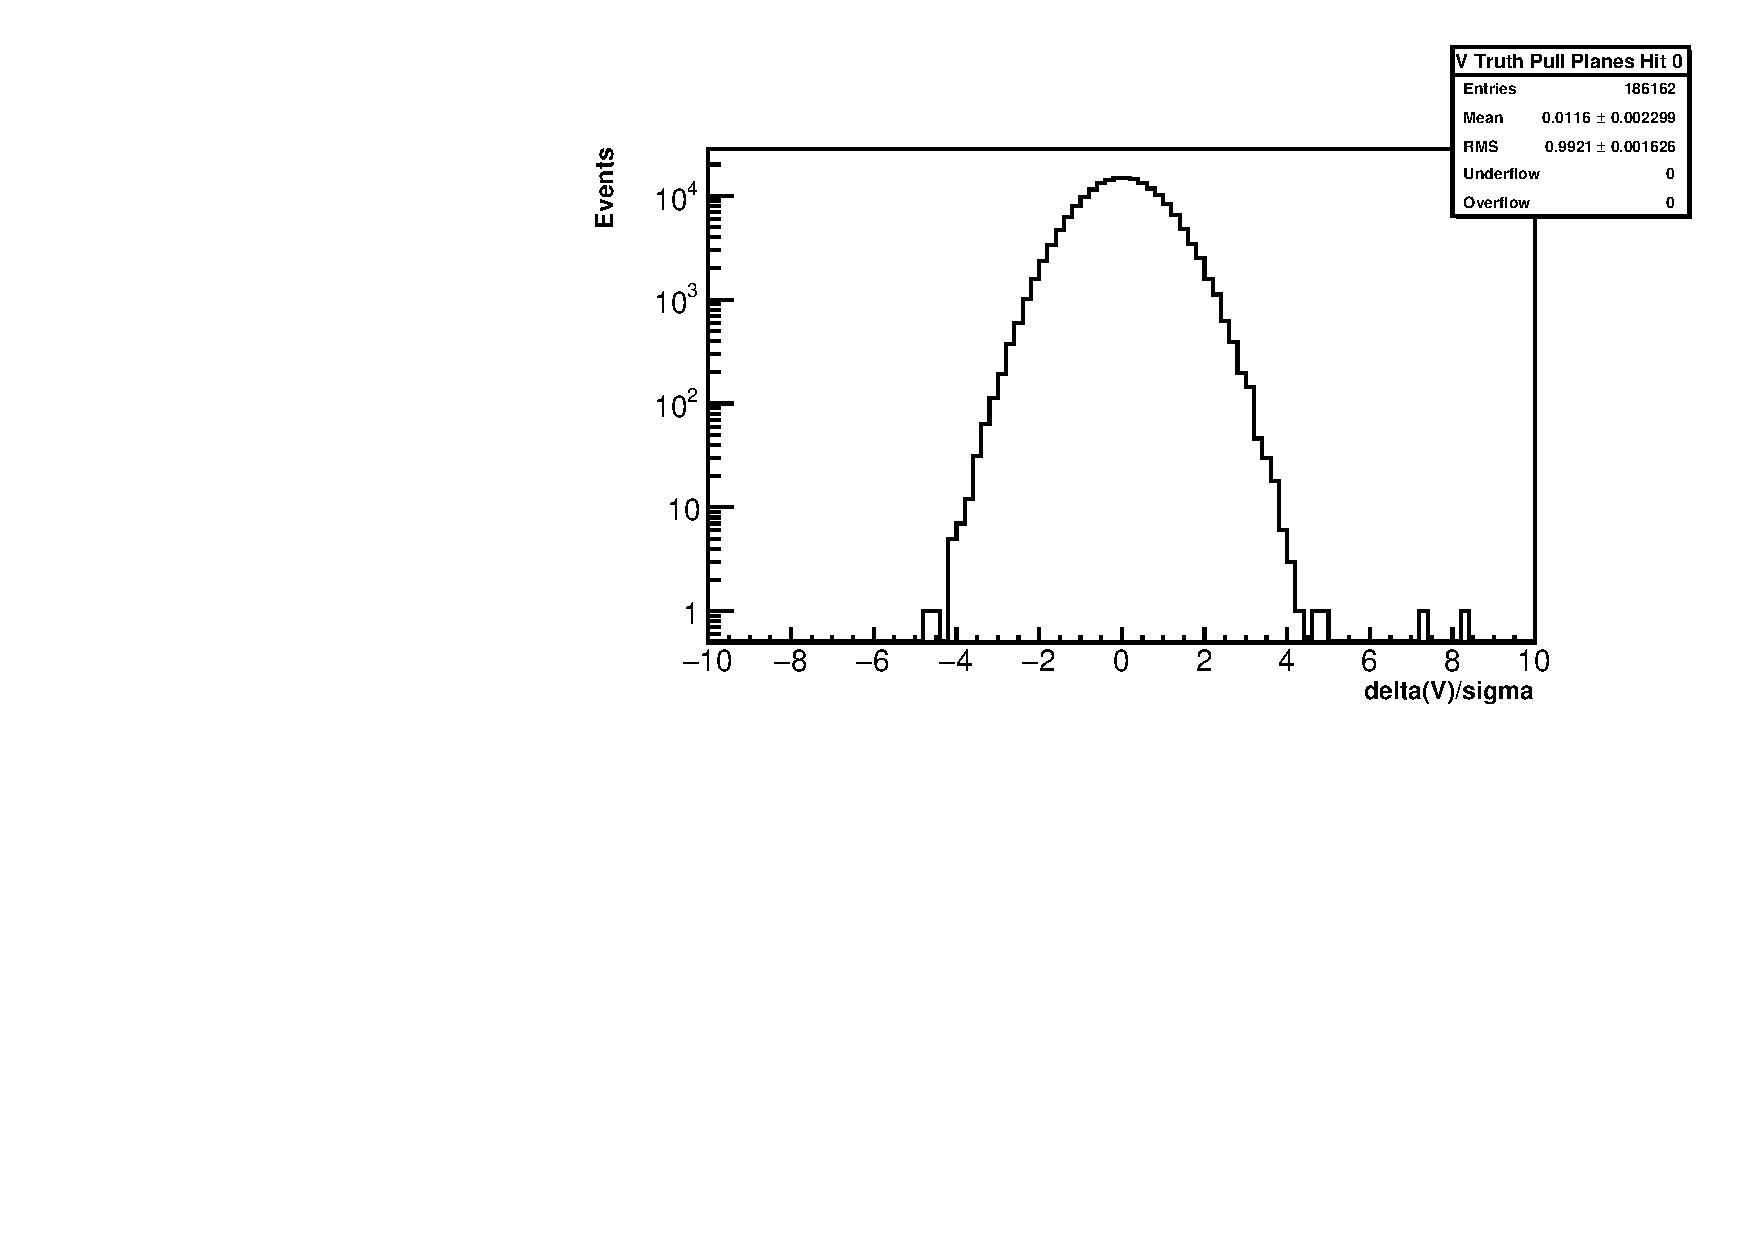
\includegraphics[width=1\textwidth]{VpullLog} 
        \caption{V truth pull on plane 0 for all tracks, log plot. Poor events can be seen as the distribution spreads out more towards the edges, with some under and overflows.}
    \end{subfigure}

    \caption{Number of iterations information.}
\end{figure}



\begin{figure}
    \centering
    \begin{subfigure}[]{0.6\textwidth}
        \centering
        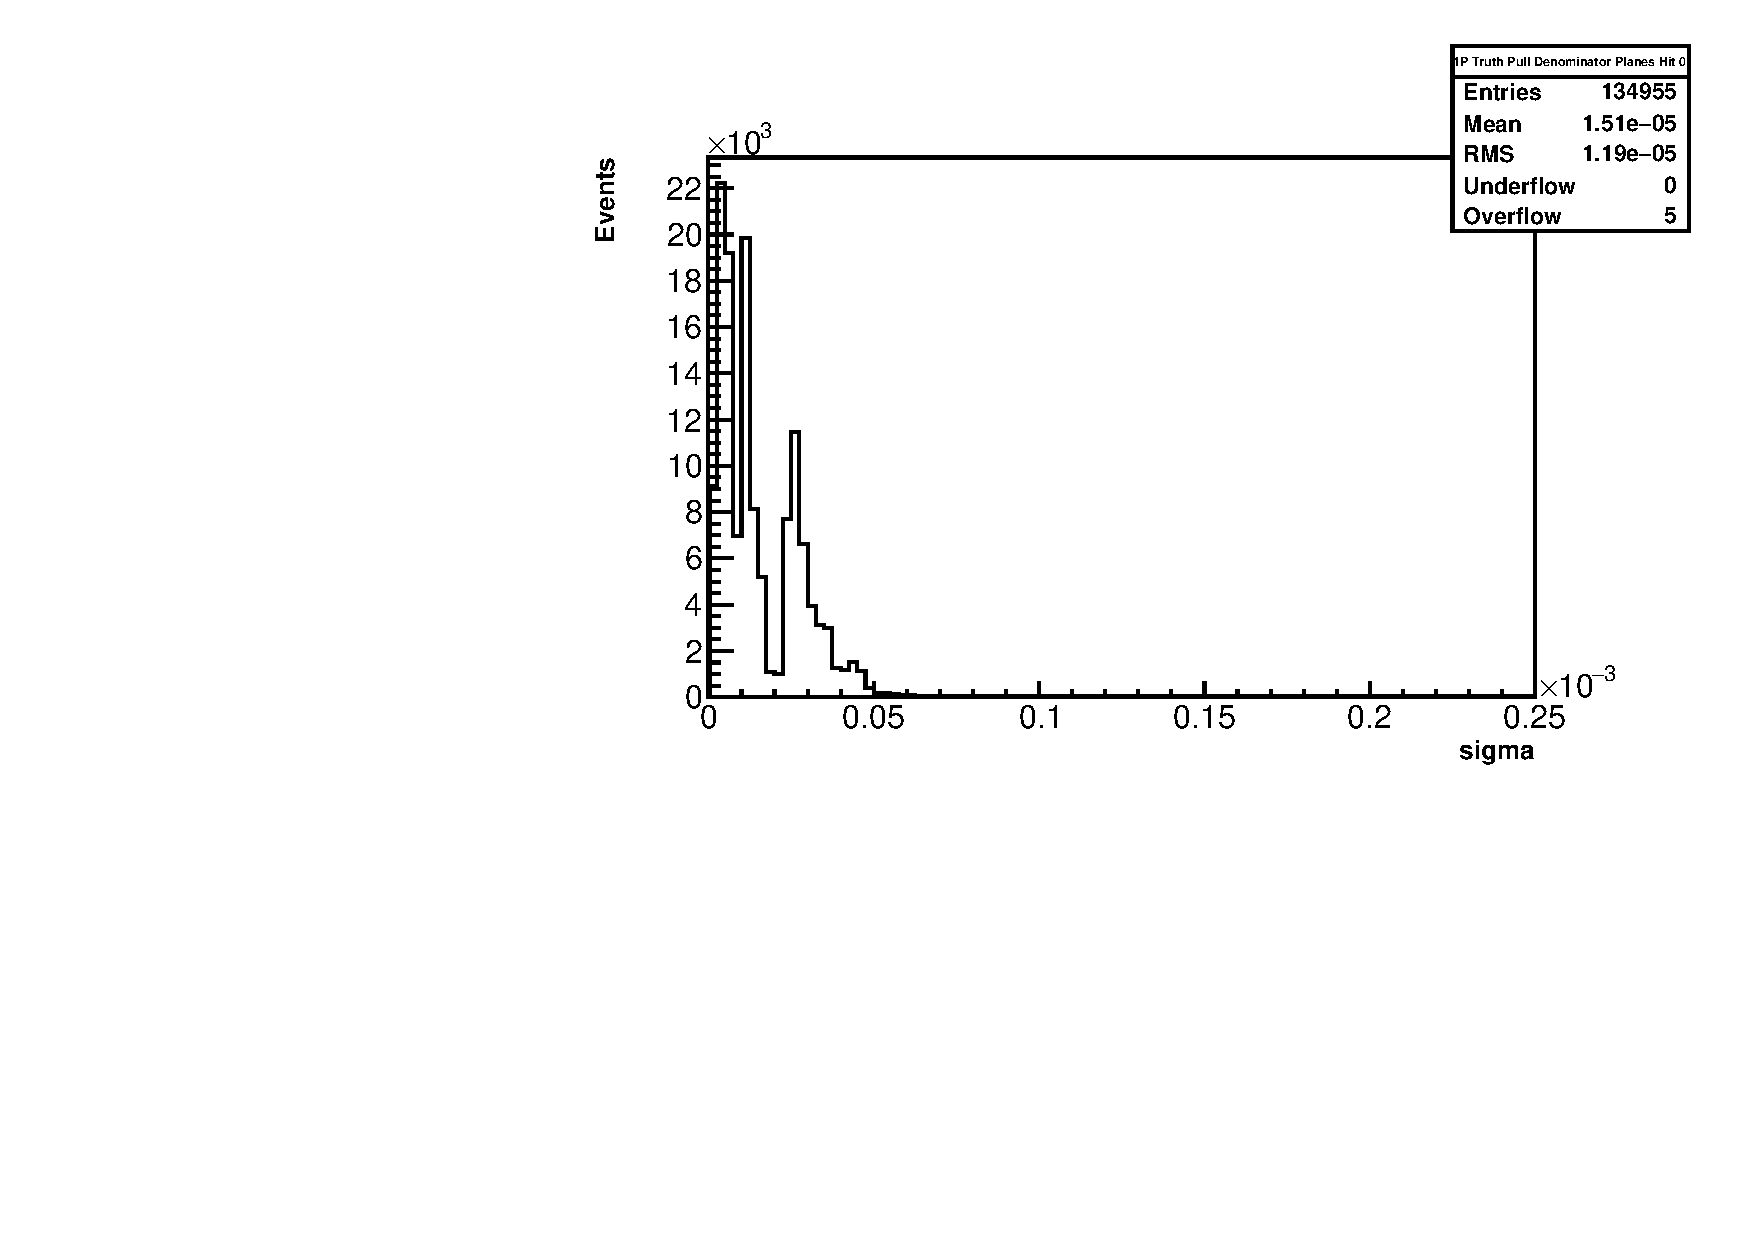
\includegraphics[width=1\textwidth]{1PpullDenom} 
        \caption{The error (denominator), in the 1/P pull. The different spikes corresponds to different numbers of planes hit, or different amounts of material passed through.}
    \end{subfigure}

    \begin{subfigure}[]{0.6\textwidth}
        \centering
        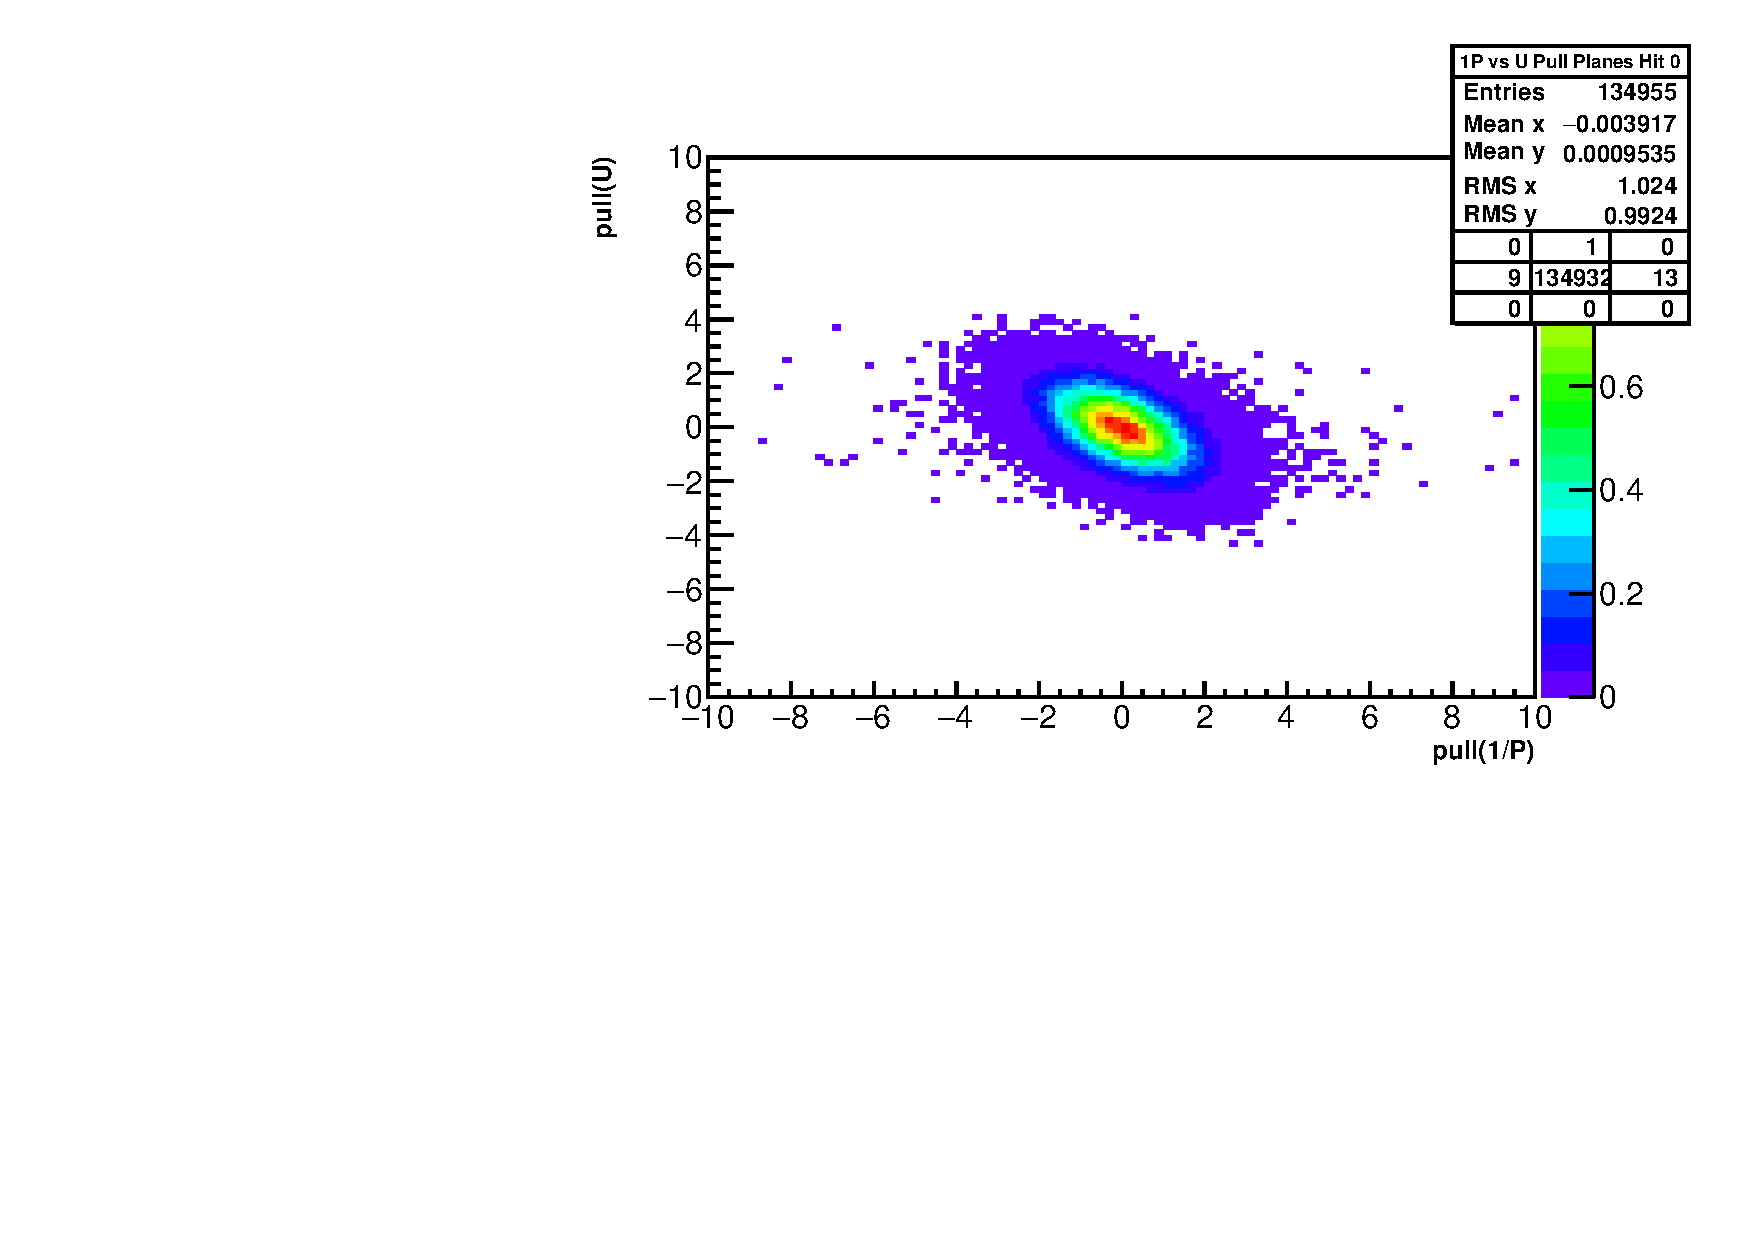
\includegraphics[width=1\textwidth]{1PpullVsUpull} 
        \caption{1/P pull vs U pull, the poor events can be seen spreading in a non-uniform way from the target.}
    \end{subfigure}
    
    \begin{subfigure}[]{0.6\textwidth}
        \centering
        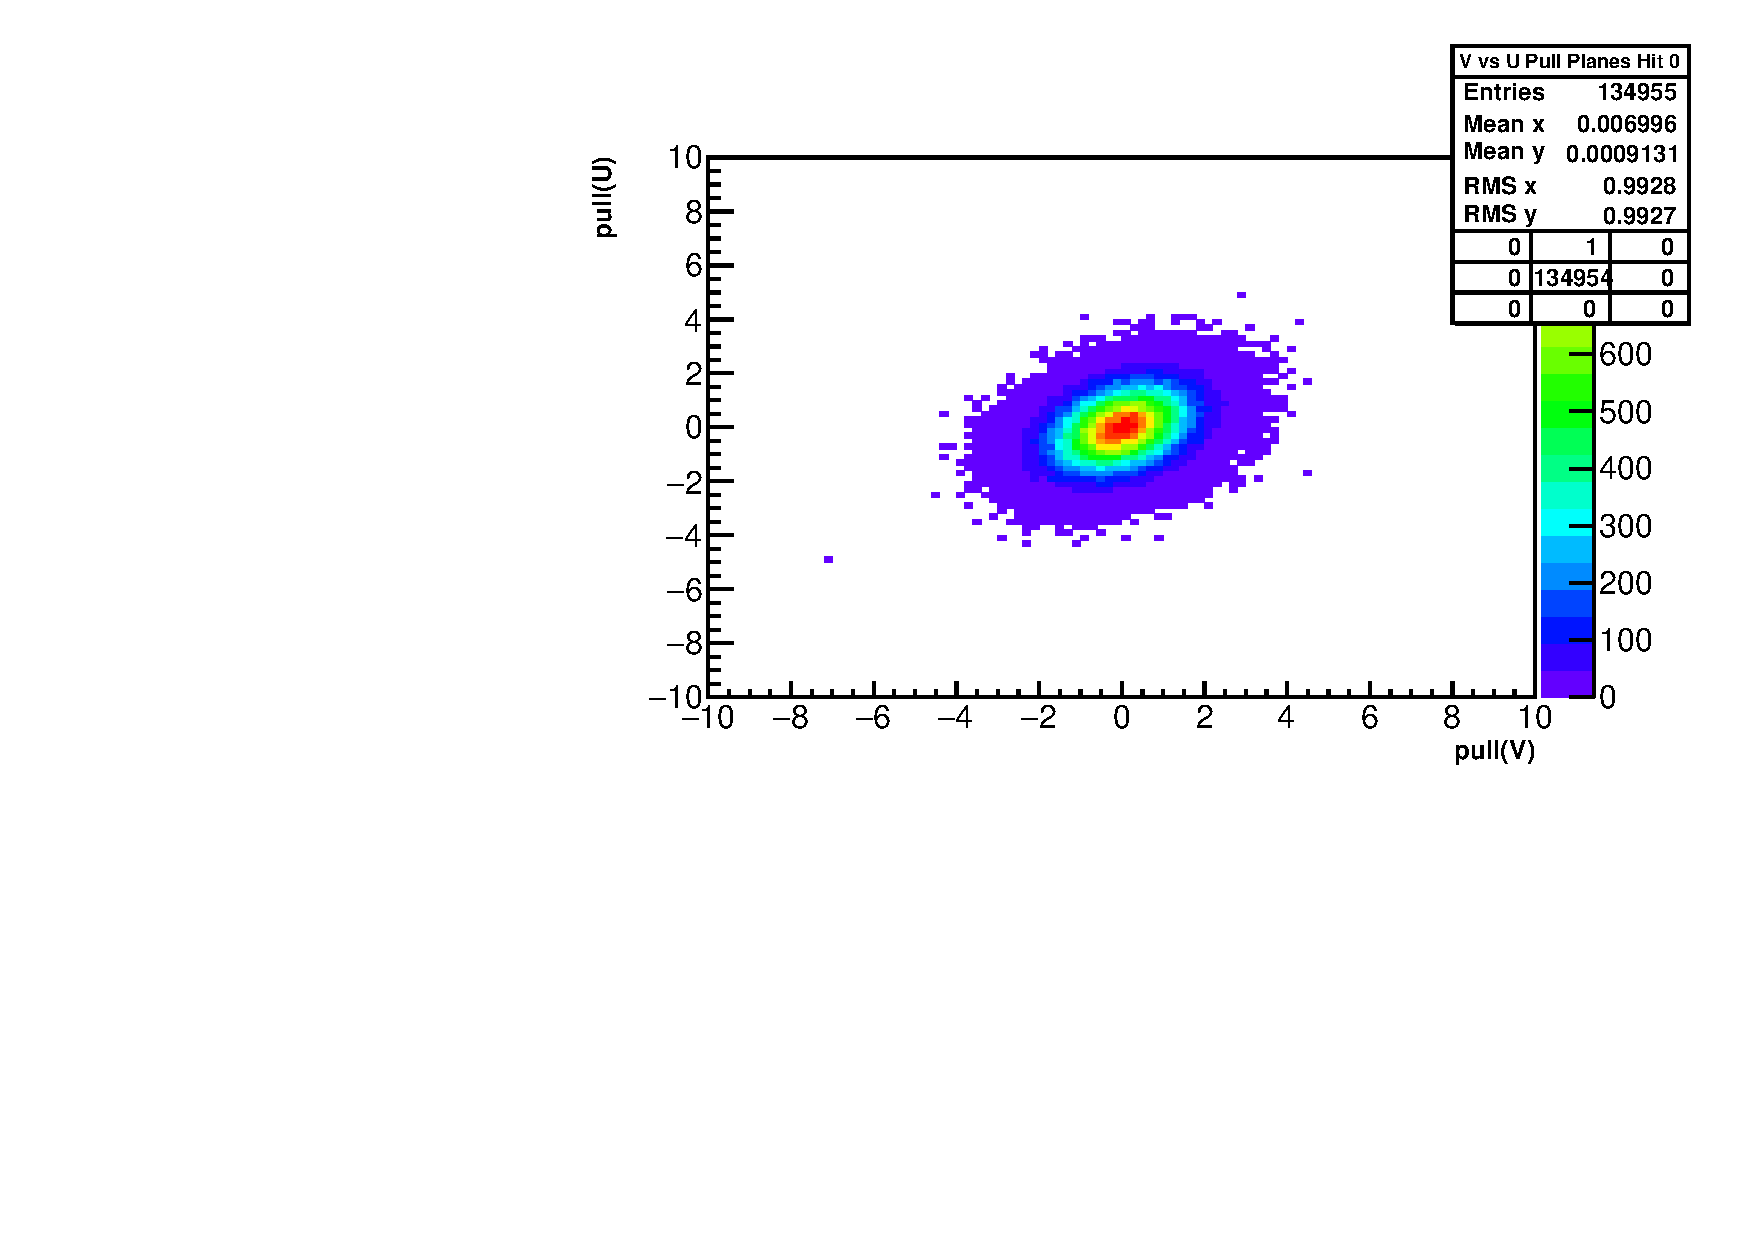
\includegraphics[width=1\textwidth]{UpullVsVpull} 
        \caption{U pull vs V pull.}
    \end{subfigure}

    \caption{Some various pull related plots.}
\end{figure}


\begin{figure}
    \centering
    \begin{subfigure}[]{0.6\textwidth}
        \centering
        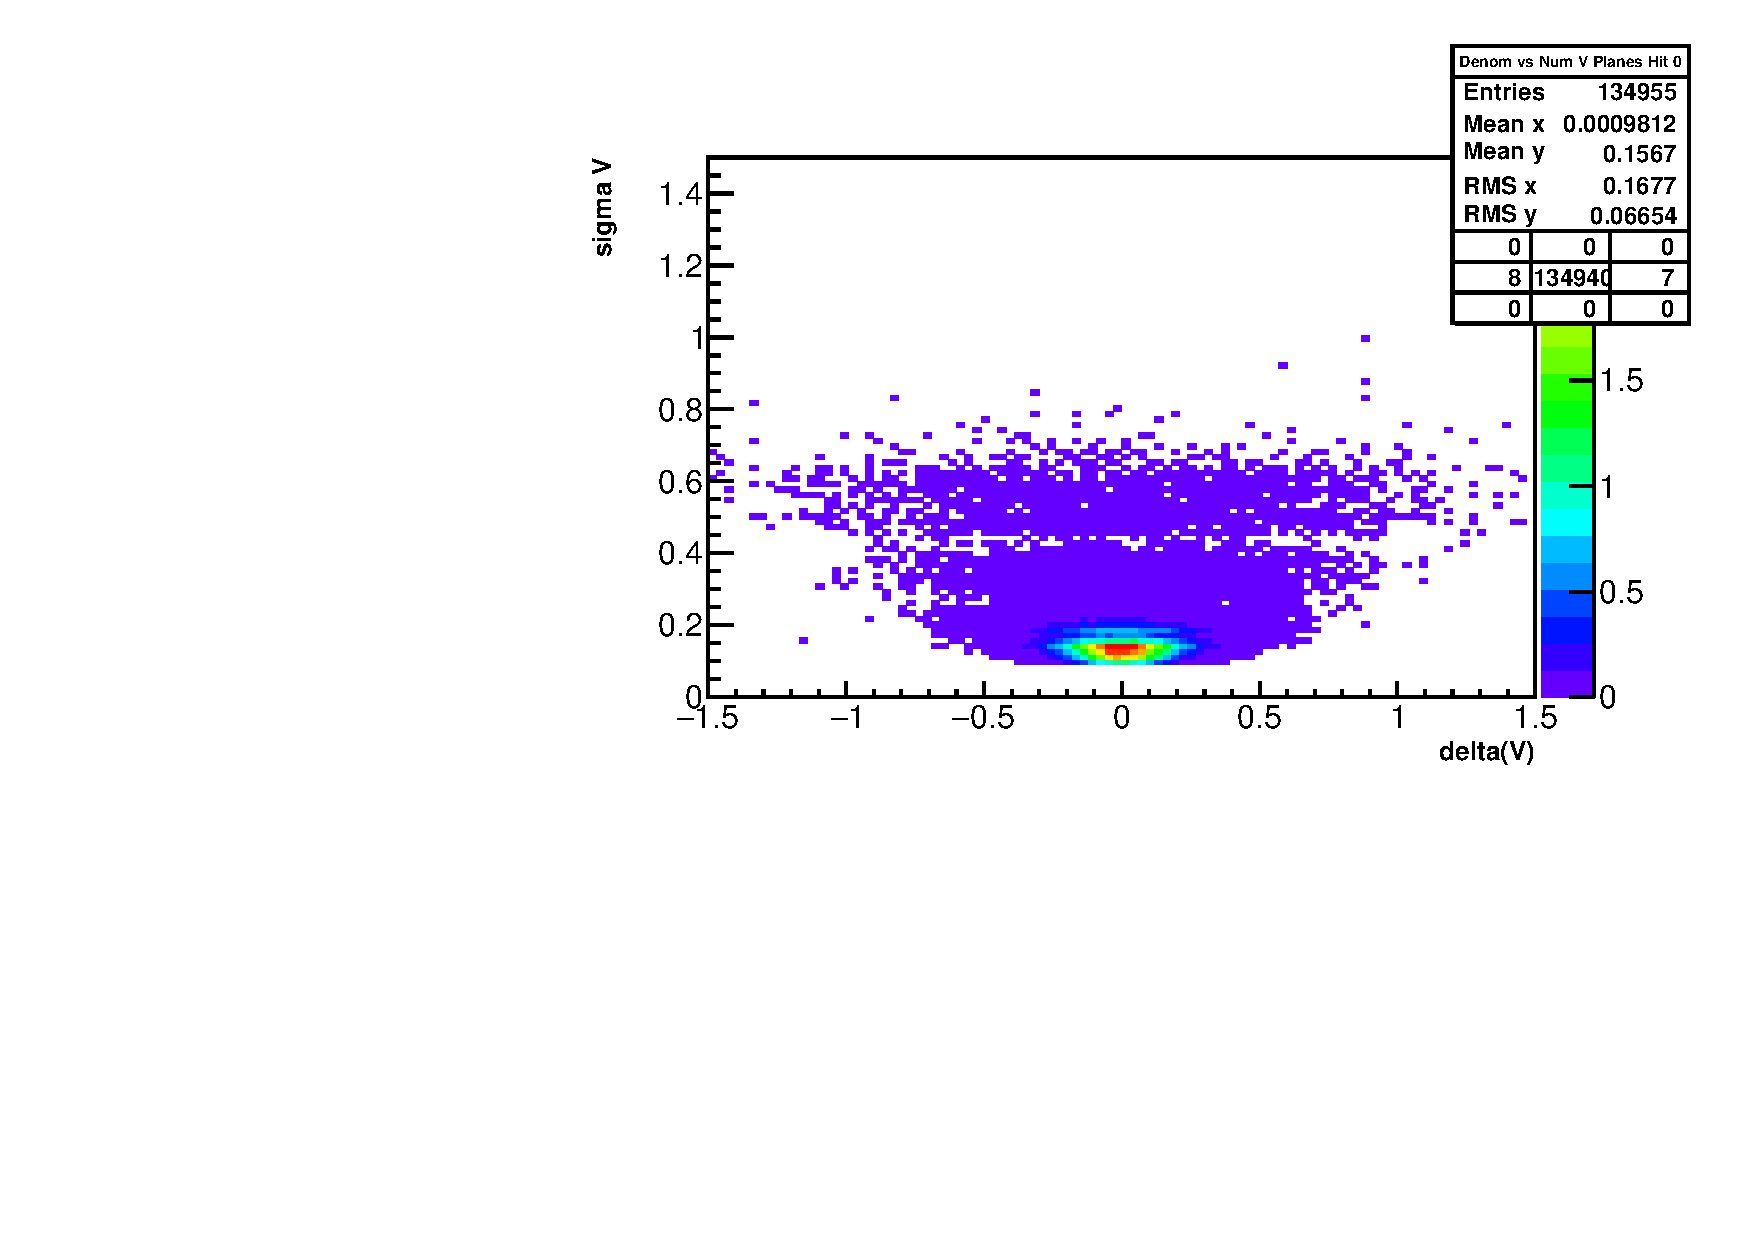
\includegraphics[width=1\textwidth]{VpullNumDenom} 
        \caption{The error in the V pull vs the residual in the V pull. The upper events are mostly comprised of tracks which hit less planes, leading to larger errors.}
    \end{subfigure}

    \begin{subfigure}[]{0.6\textwidth}
        \centering
        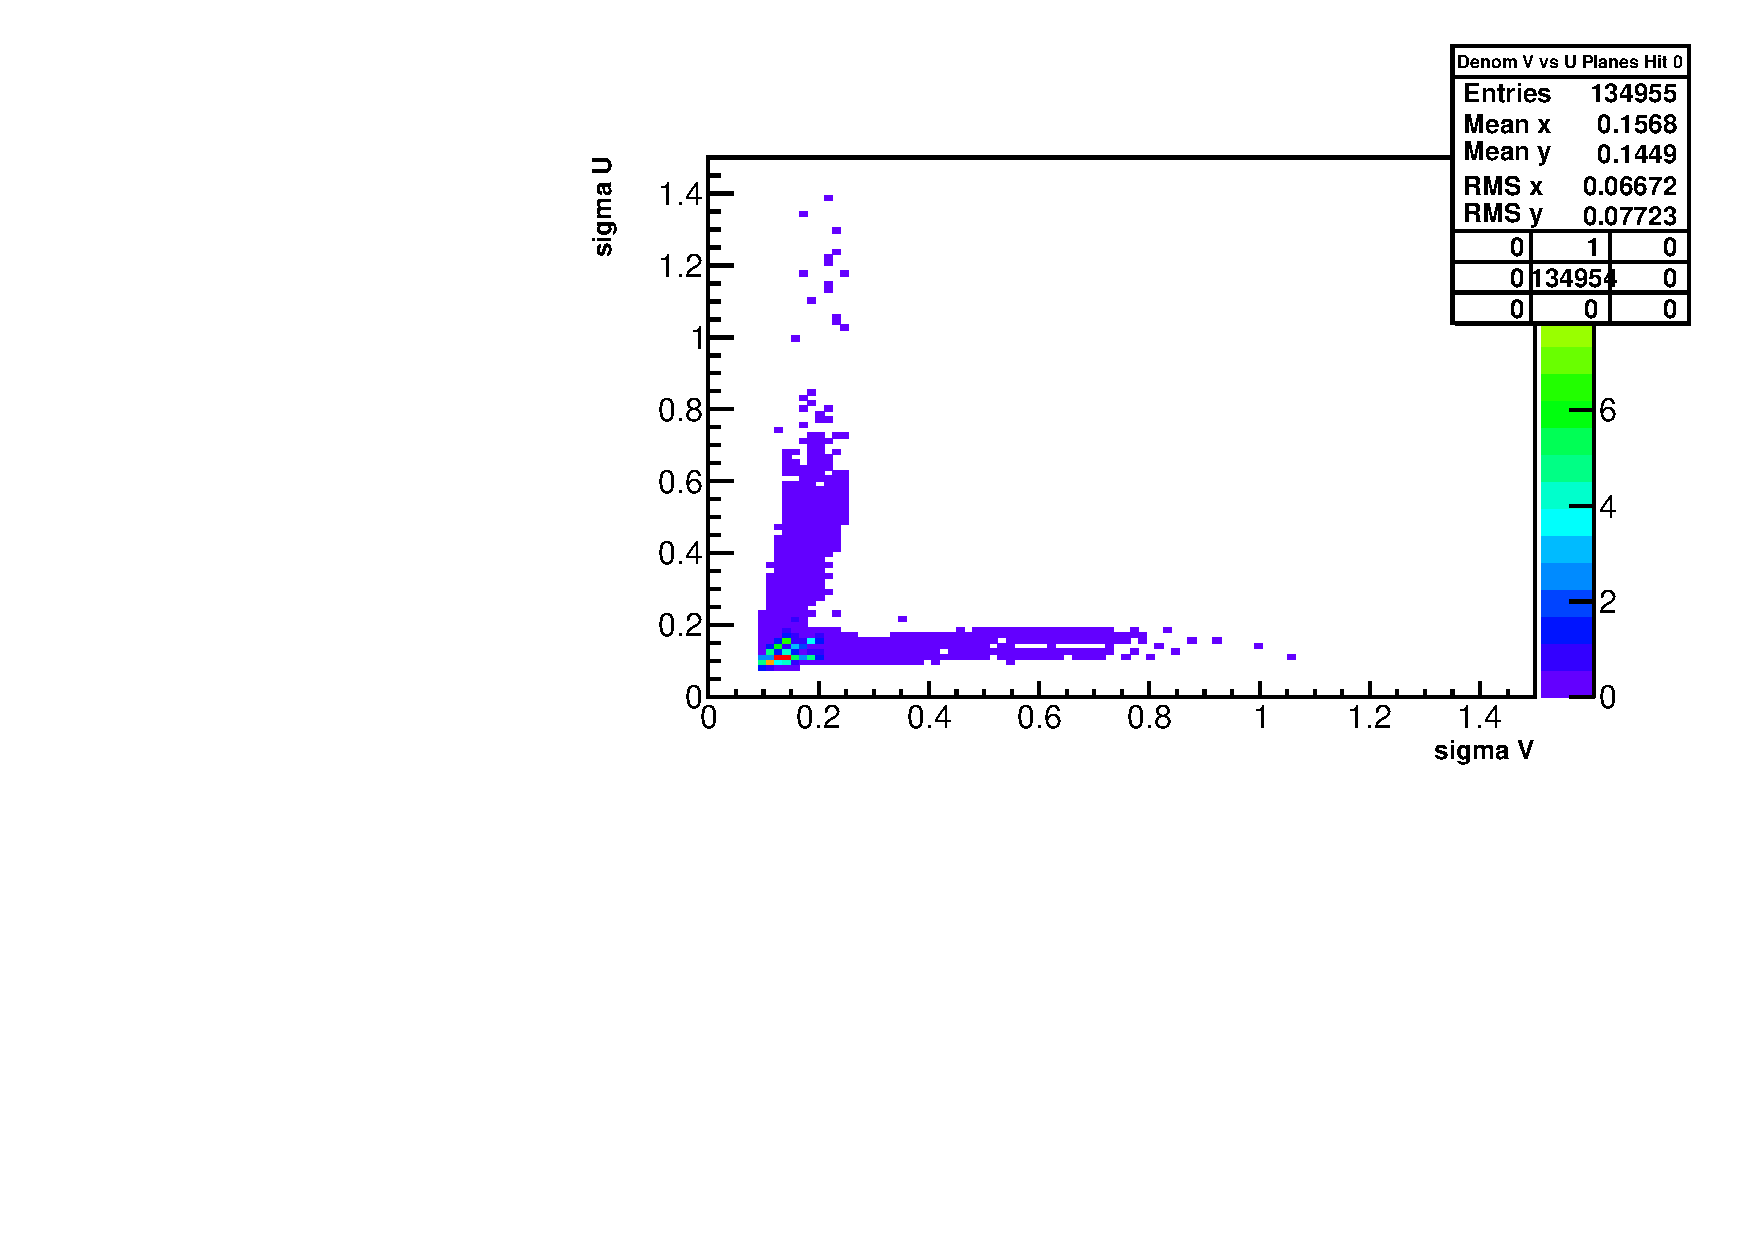
\includegraphics[width=1\textwidth]{DenomUV} 
        \caption{Error in U pull vs error in V pull, can be seen to be mostly uncorrelated within the fit.}
    \end{subfigure}
    
    \begin{subfigure}[]{0.6\textwidth}
        \centering
        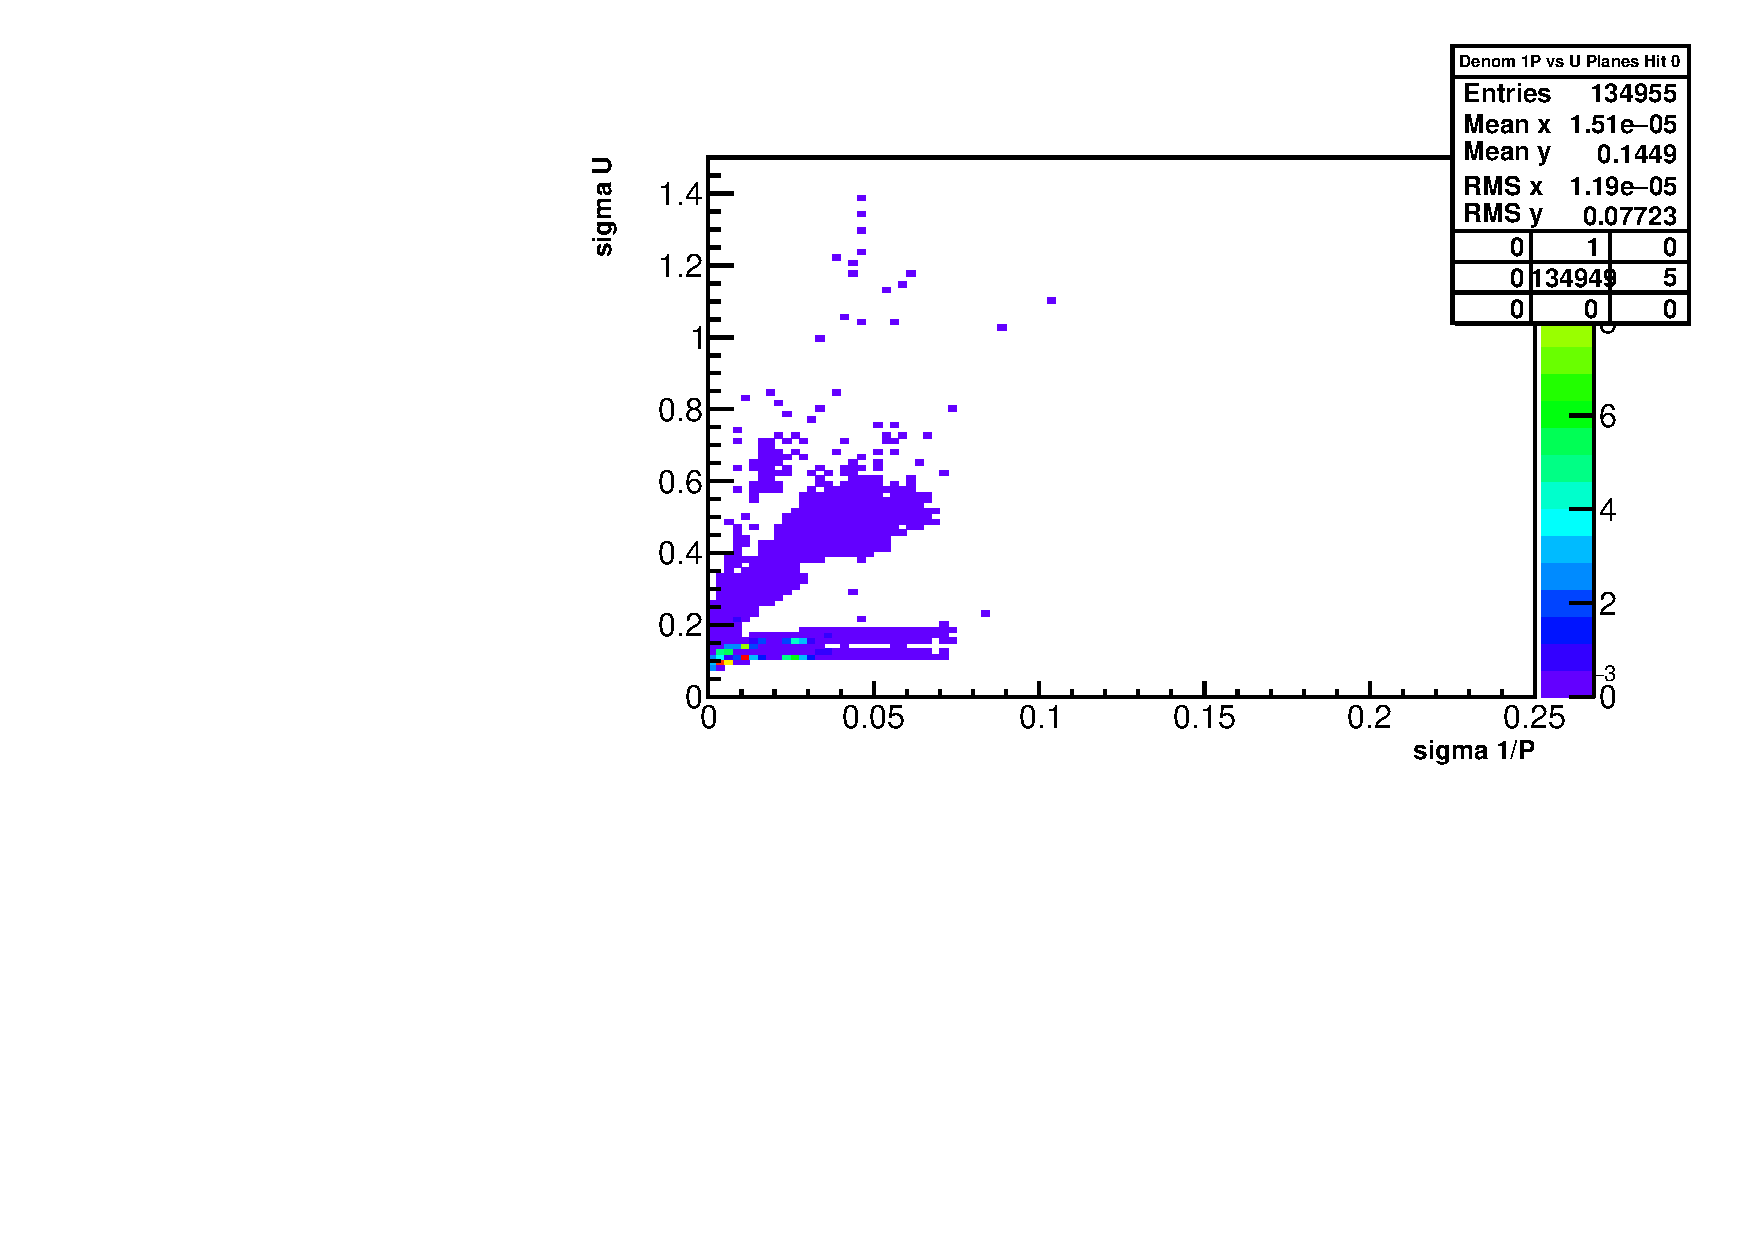
\includegraphics[width=1\textwidth]{Denom1PU} 
        \caption{Error in U pull vs error in 1/P pull. Some interesting structure is observed, that is not fully understood.}
    \end{subfigure}

    \caption{Some various pull related plots.}
\end{figure}



\begin{figure}
    \centering
    \begin{subfigure}[]{0.5\textwidth}
        \centering
        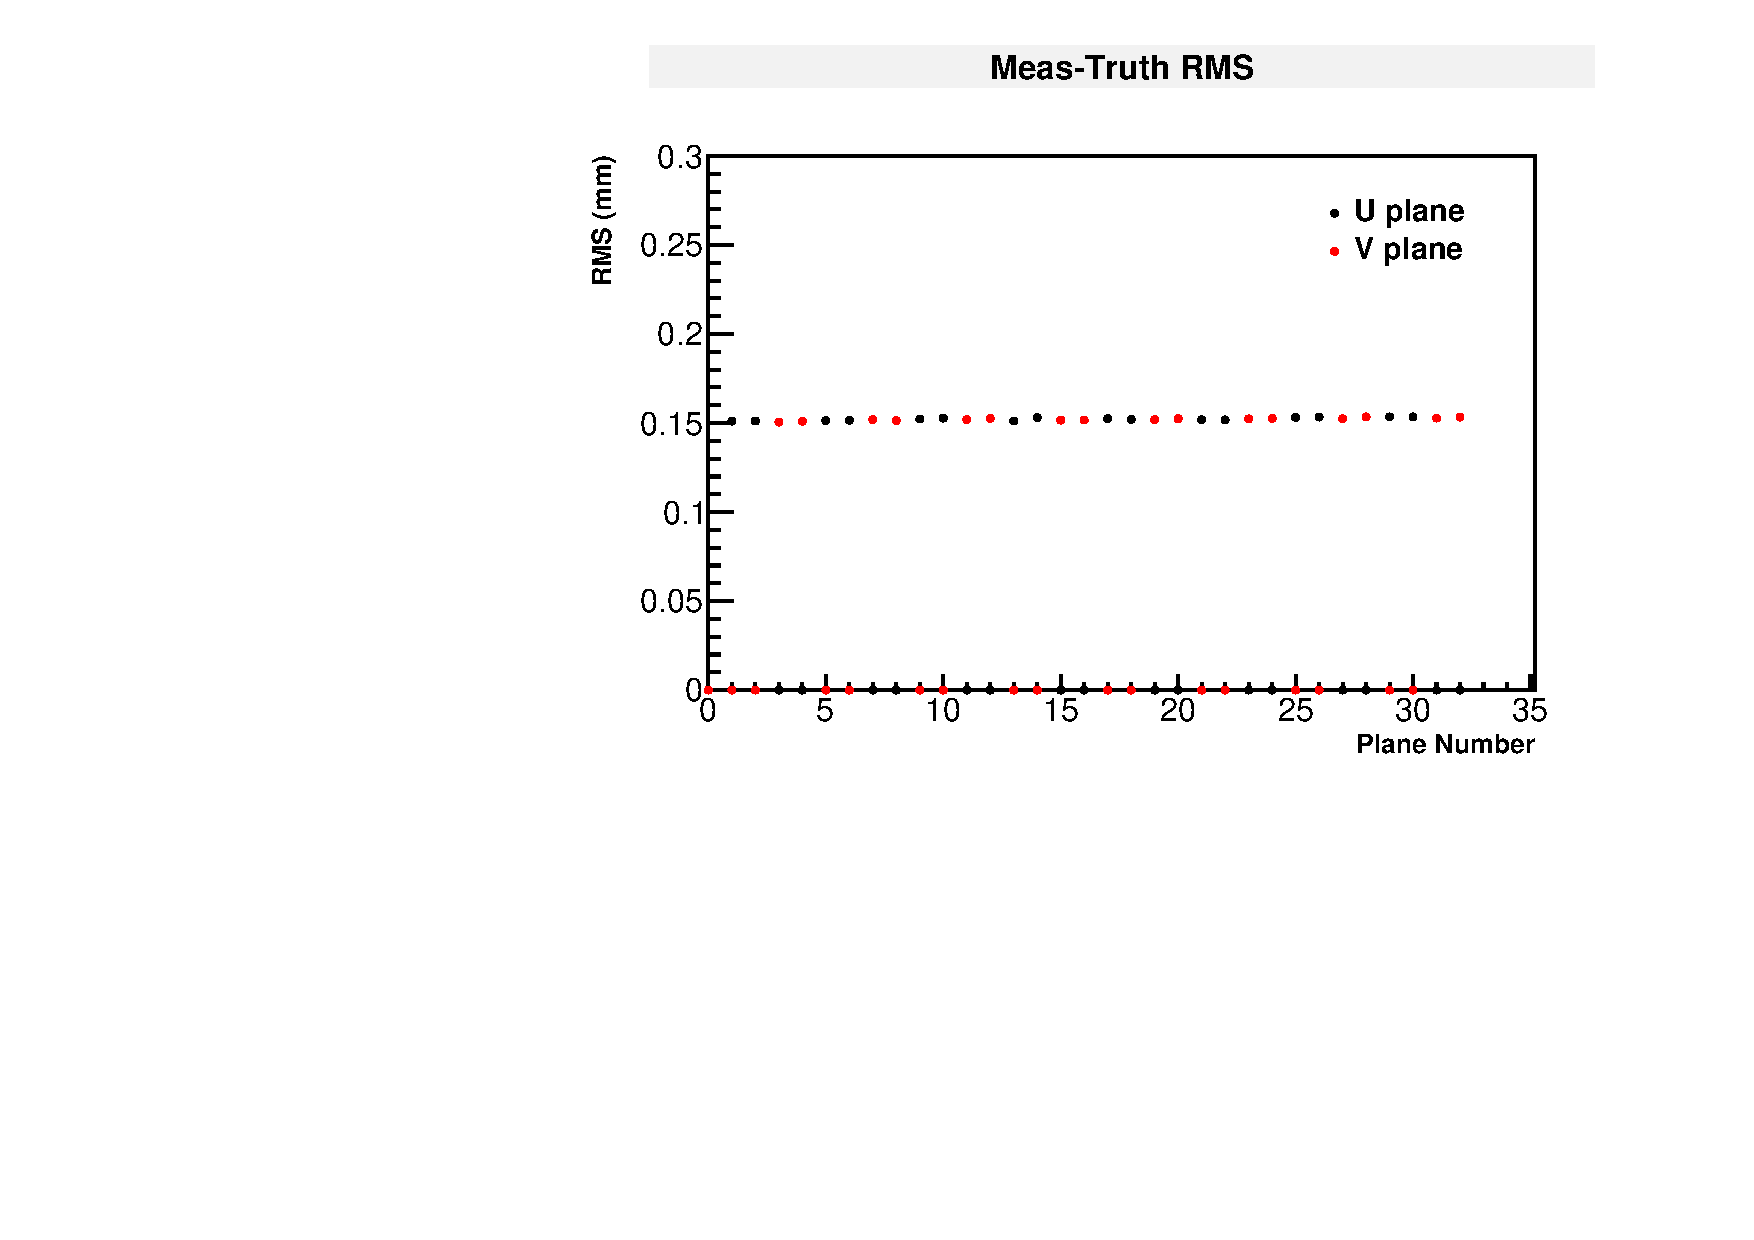
\includegraphics[width=1\textwidth]{meastruthrms} 
        \caption{RMS of measured - truth residuals, the input 150 $\mu$m smearing can be seen. Points on the X axis signify no measurement of that parameter on that plane.}
    \end{subfigure}

    \begin{subfigure}[]{0.5\textwidth}
        \centering
        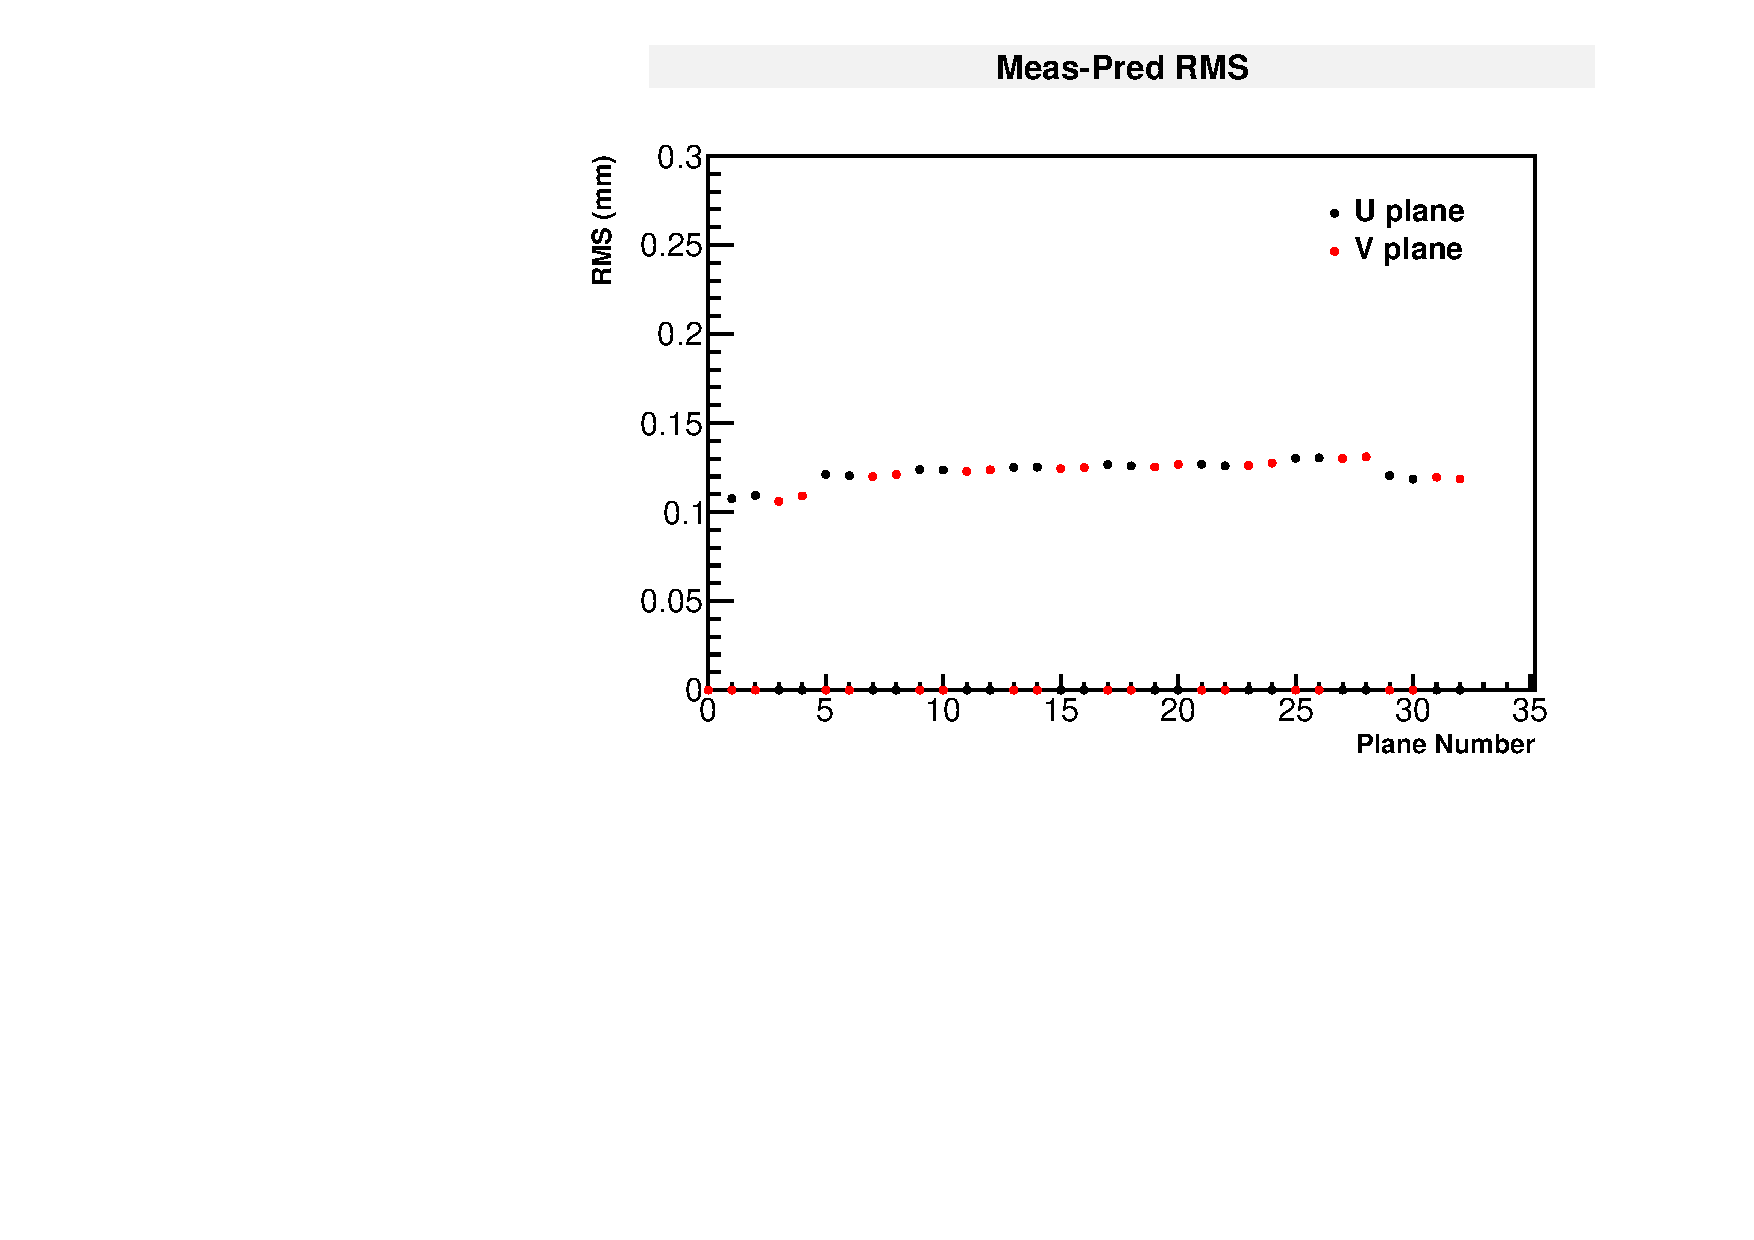
\includegraphics[width=1\textwidth]{measpredrms} 
        \caption{RMS of measured - predicted residuals. There is an overall upside down parabolic shape to the distribution. A slight rise towards higher plane number indicates larger error due to increased material.}
    \end{subfigure}
    
    \begin{subfigure}[]{0.5\textwidth}
        \centering
        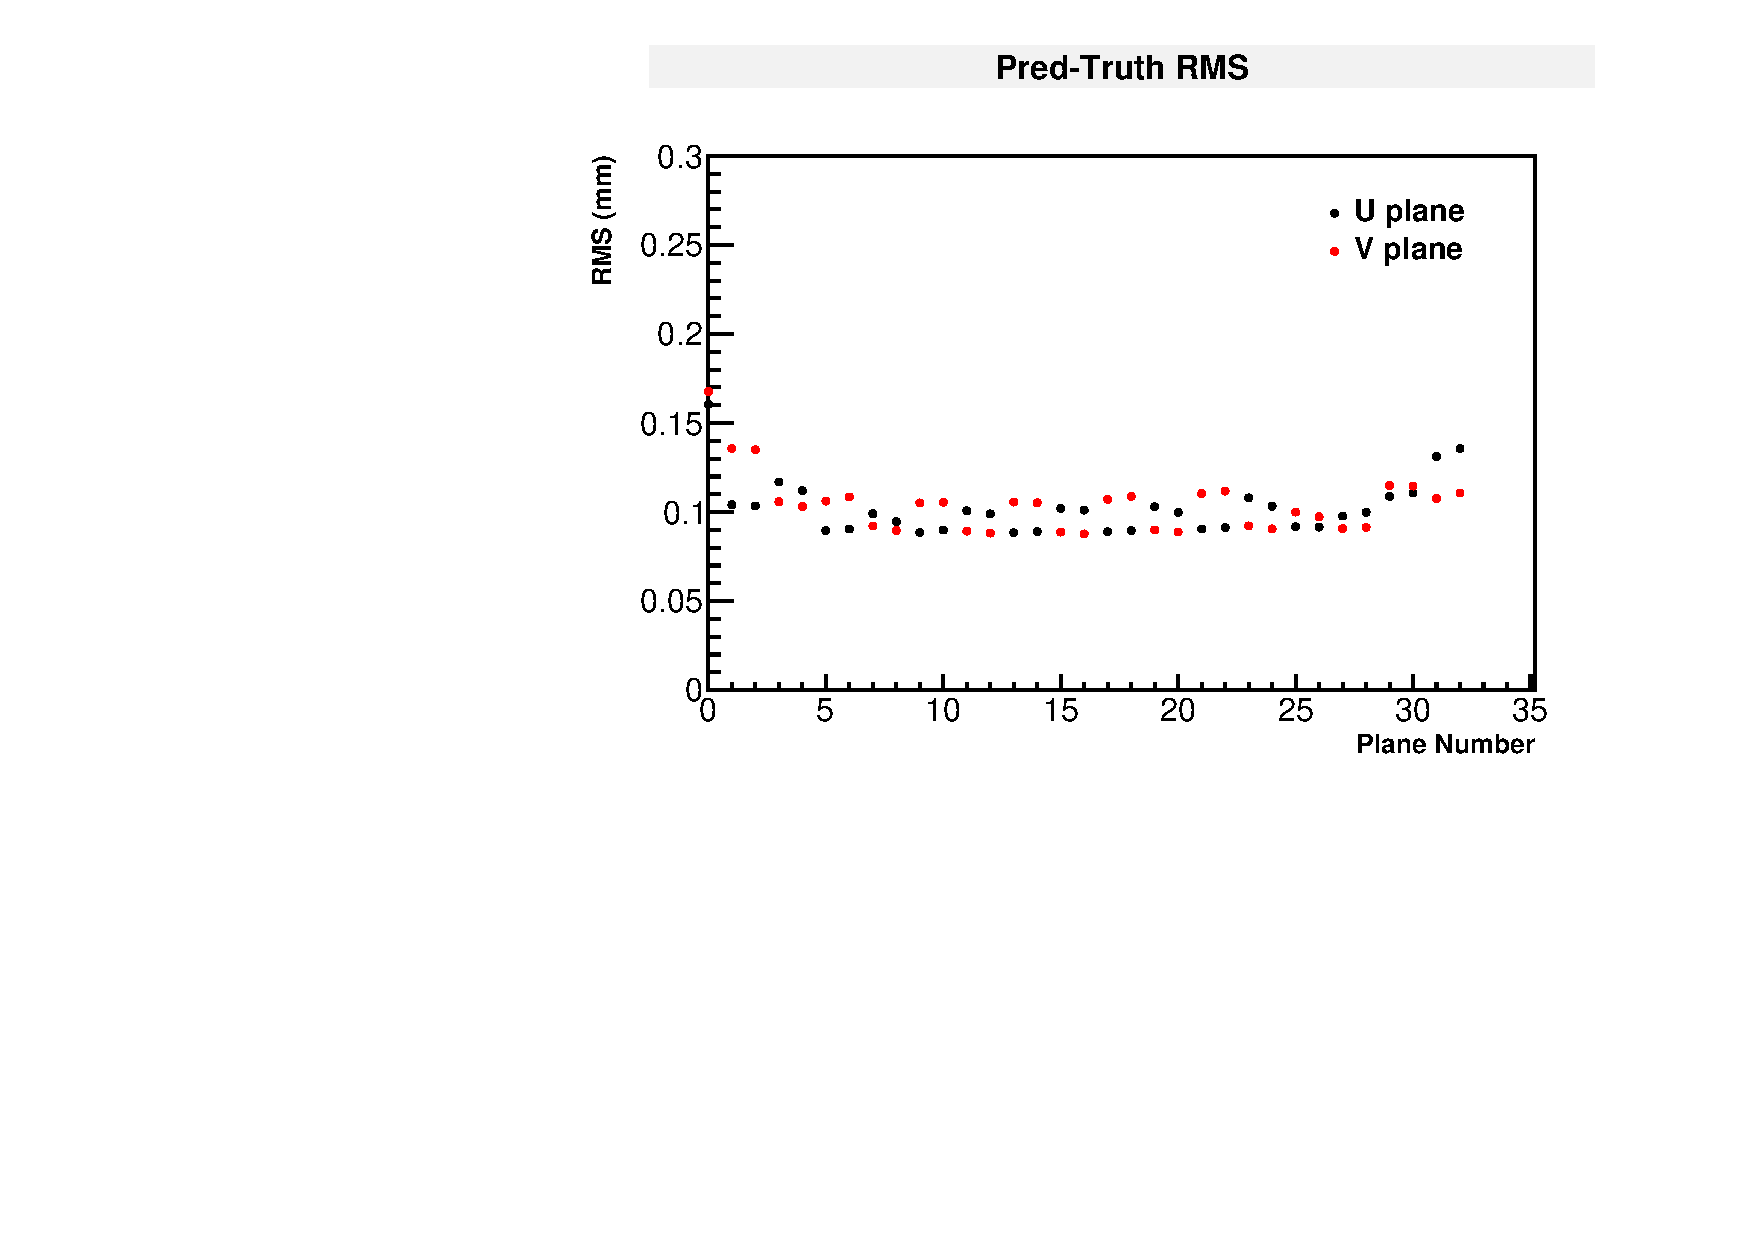
\includegraphics[width=1\textwidth]{predtruthrms} 
        \caption{RMS of predicted - truth residuals. There is an overall parabolic shape to the distribution, comprised of many parabolas. The RMS at the center of the fit is better than the edges since there are more measurements near the center. On individual planes, whatever that plane measured will have a better RMS, eg. plane 1 which is a U plane fits U better than V at that plane.}
    \end{subfigure}

    \caption{RMS of residual plots as a function of plane number for all events. Technically these should be split up according to number of planes hit, and the distance between the first and last hit in the fit, which would simplify and justify the shapes. See \href{http://gm2-docdb.fnal.gov:8080/cgi-bin/ShowDocument?docid=3813}{DocDB 3813} and \href{http://gm2-docdb.fnal.gov:8080/cgi-bin/ShowDocument?docid=6306}{DocDB 6306} to understand these plots.}
\end{figure}



\begin{figure}
    \centering
    \begin{subfigure}[]{0.6\textwidth}
        \centering
        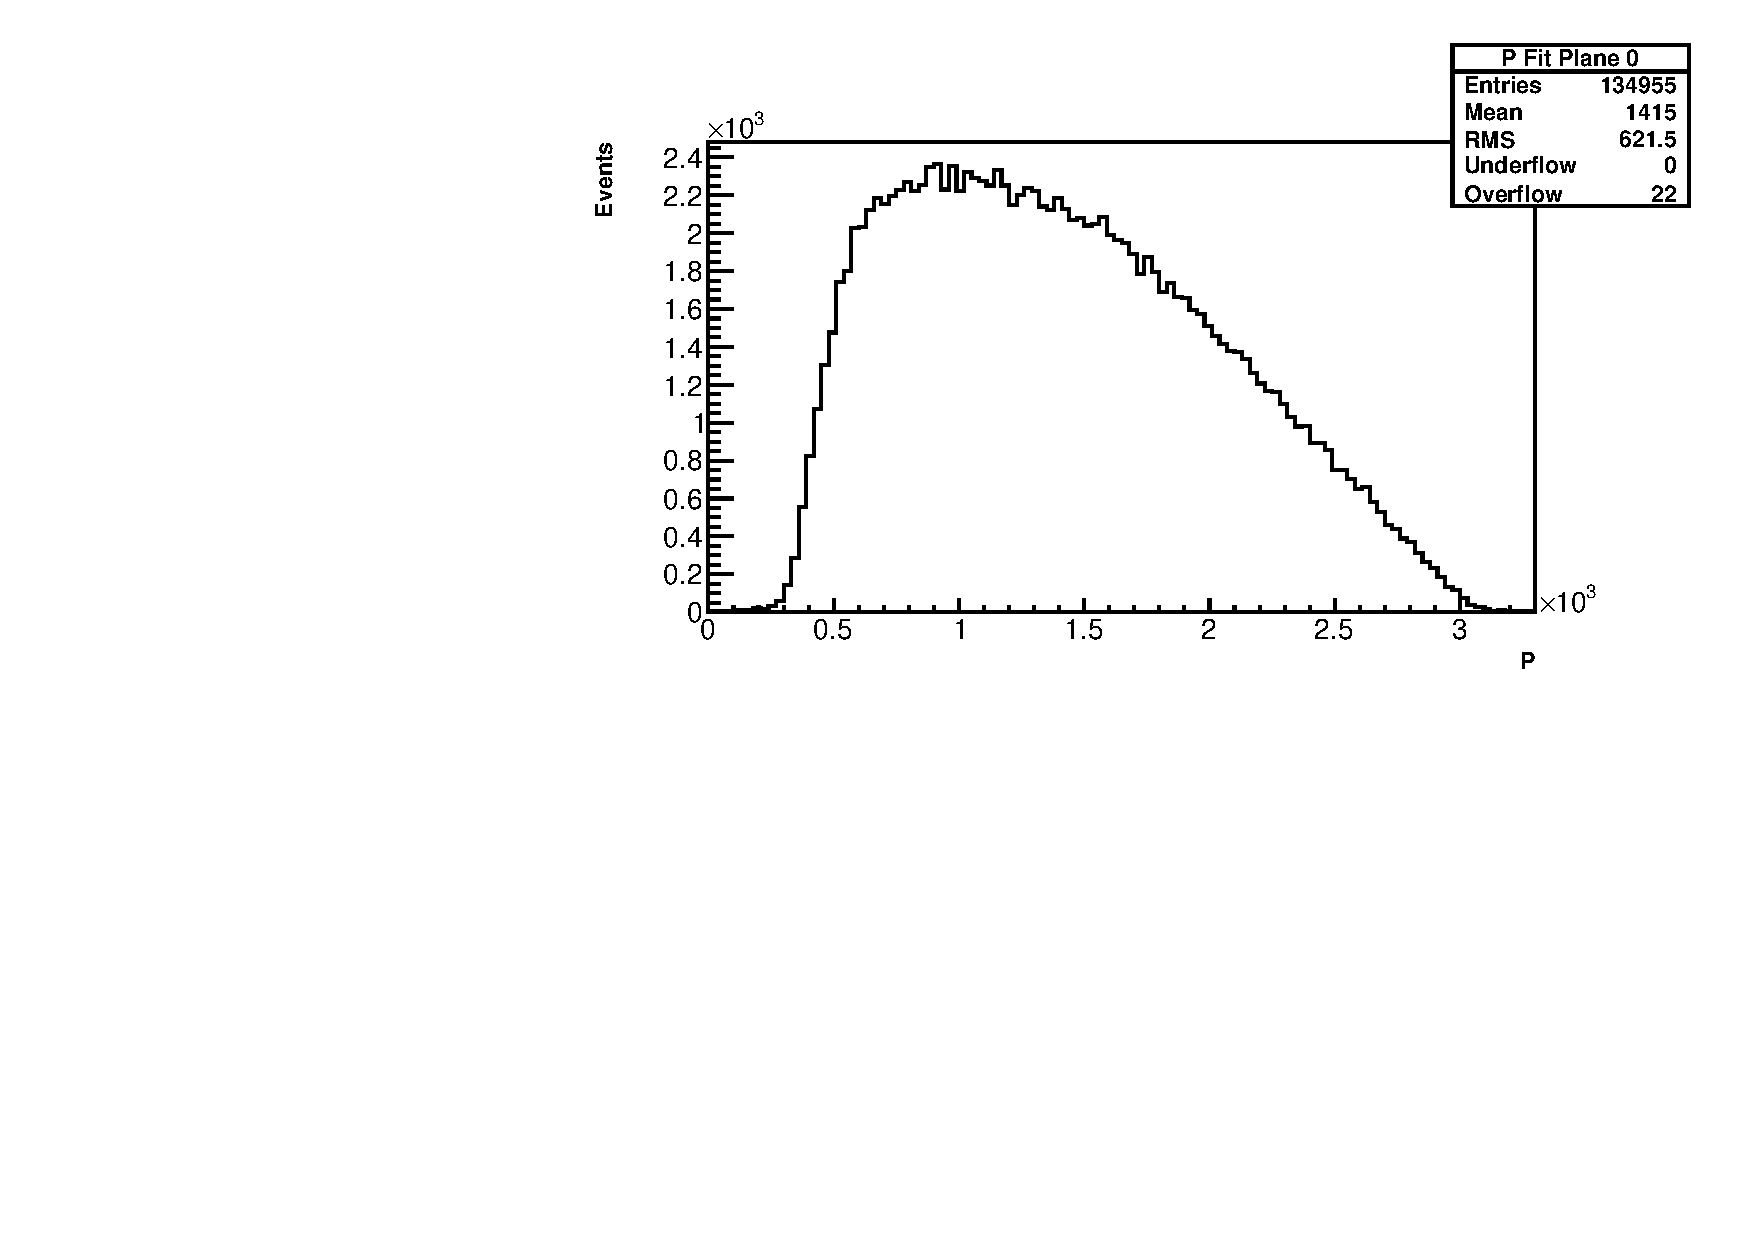
\includegraphics[width=1\textwidth]{Pplane0} 
        \caption{Momentum magnitude from the fit at plane 0. X momentum distribution is very similar to this since most of the momentum is in the forward direction.}
    \end{subfigure}

    \begin{subfigure}[]{0.6\textwidth}
        \centering
        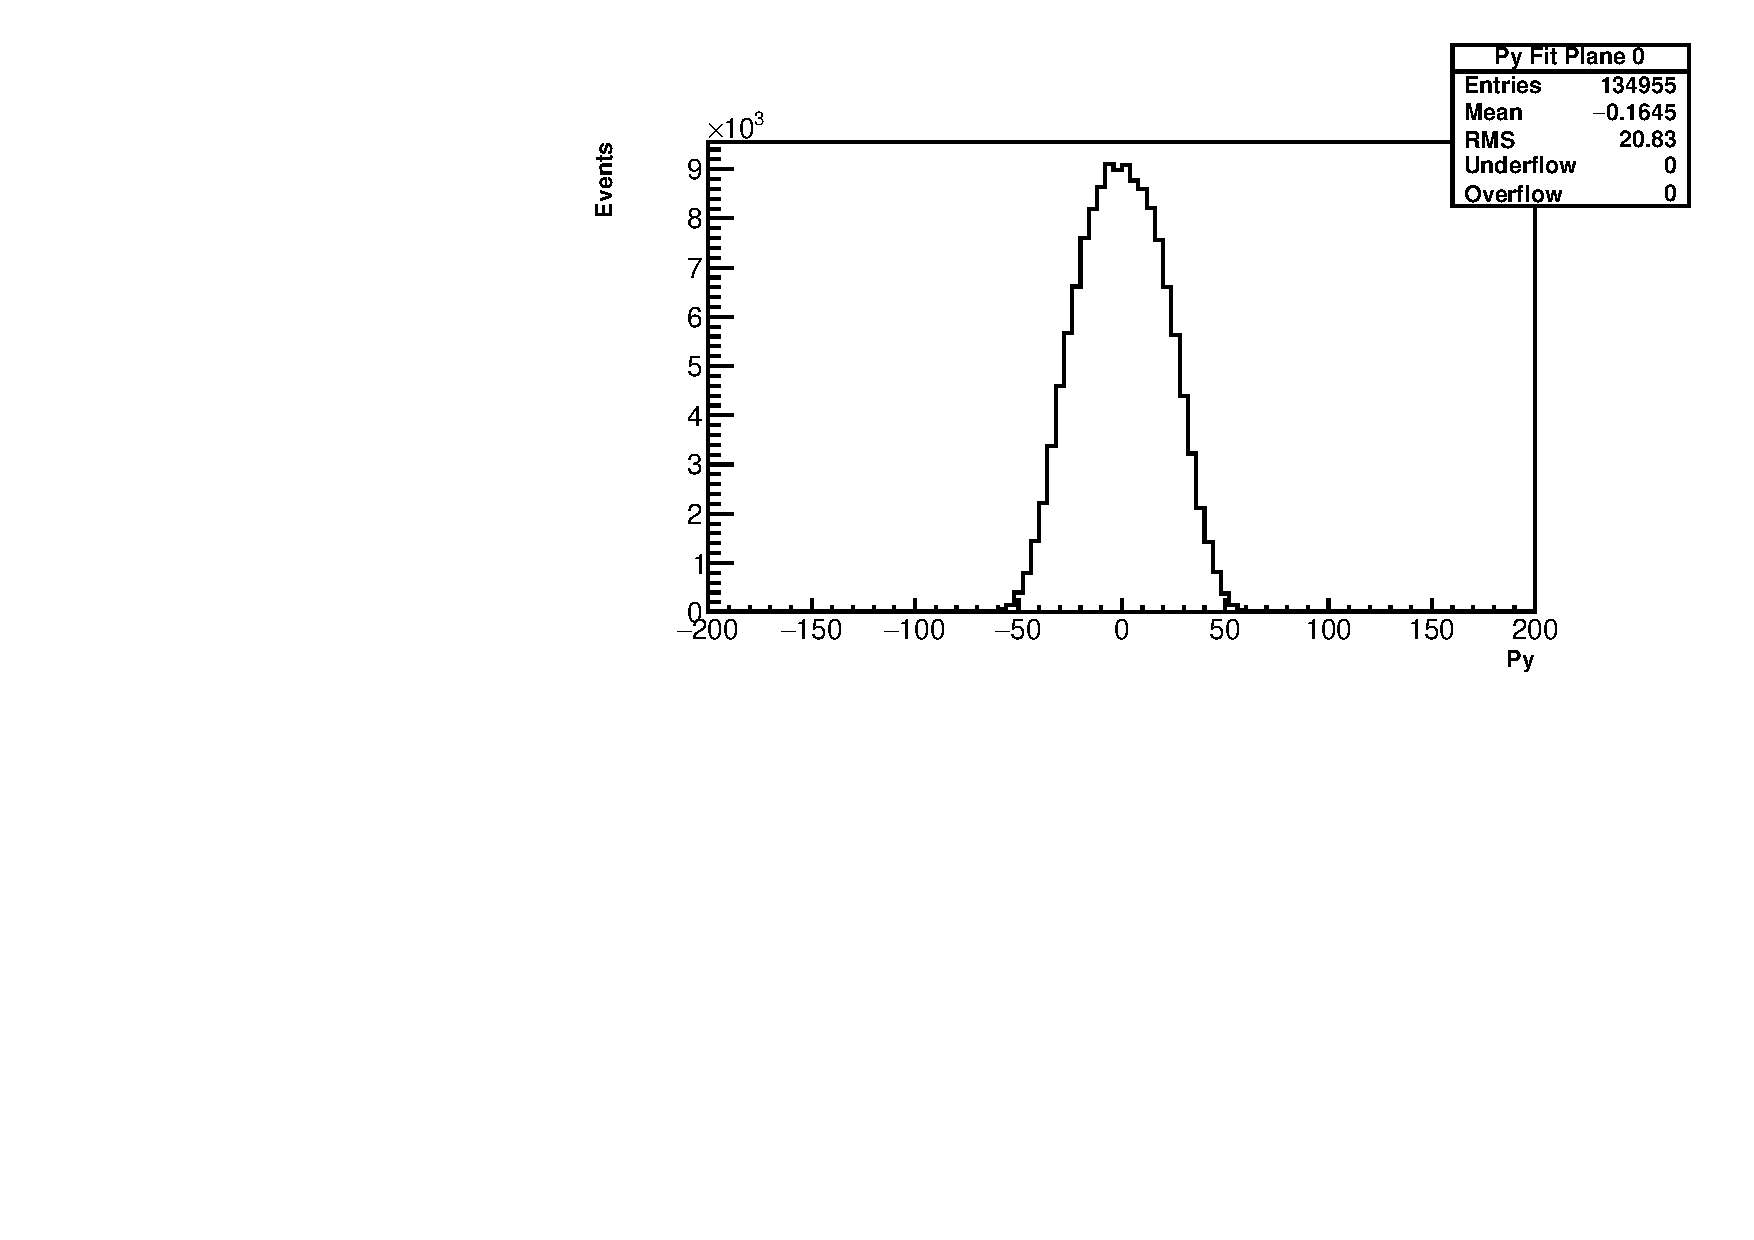
\includegraphics[width=1\textwidth]{Pyplane0} 
        \caption{Y momentum from the fit at plane 0. Bounded nicely by the measurement range of the detectors.}
    \end{subfigure}
    
    \begin{subfigure}[]{0.6\textwidth}
        \centering
        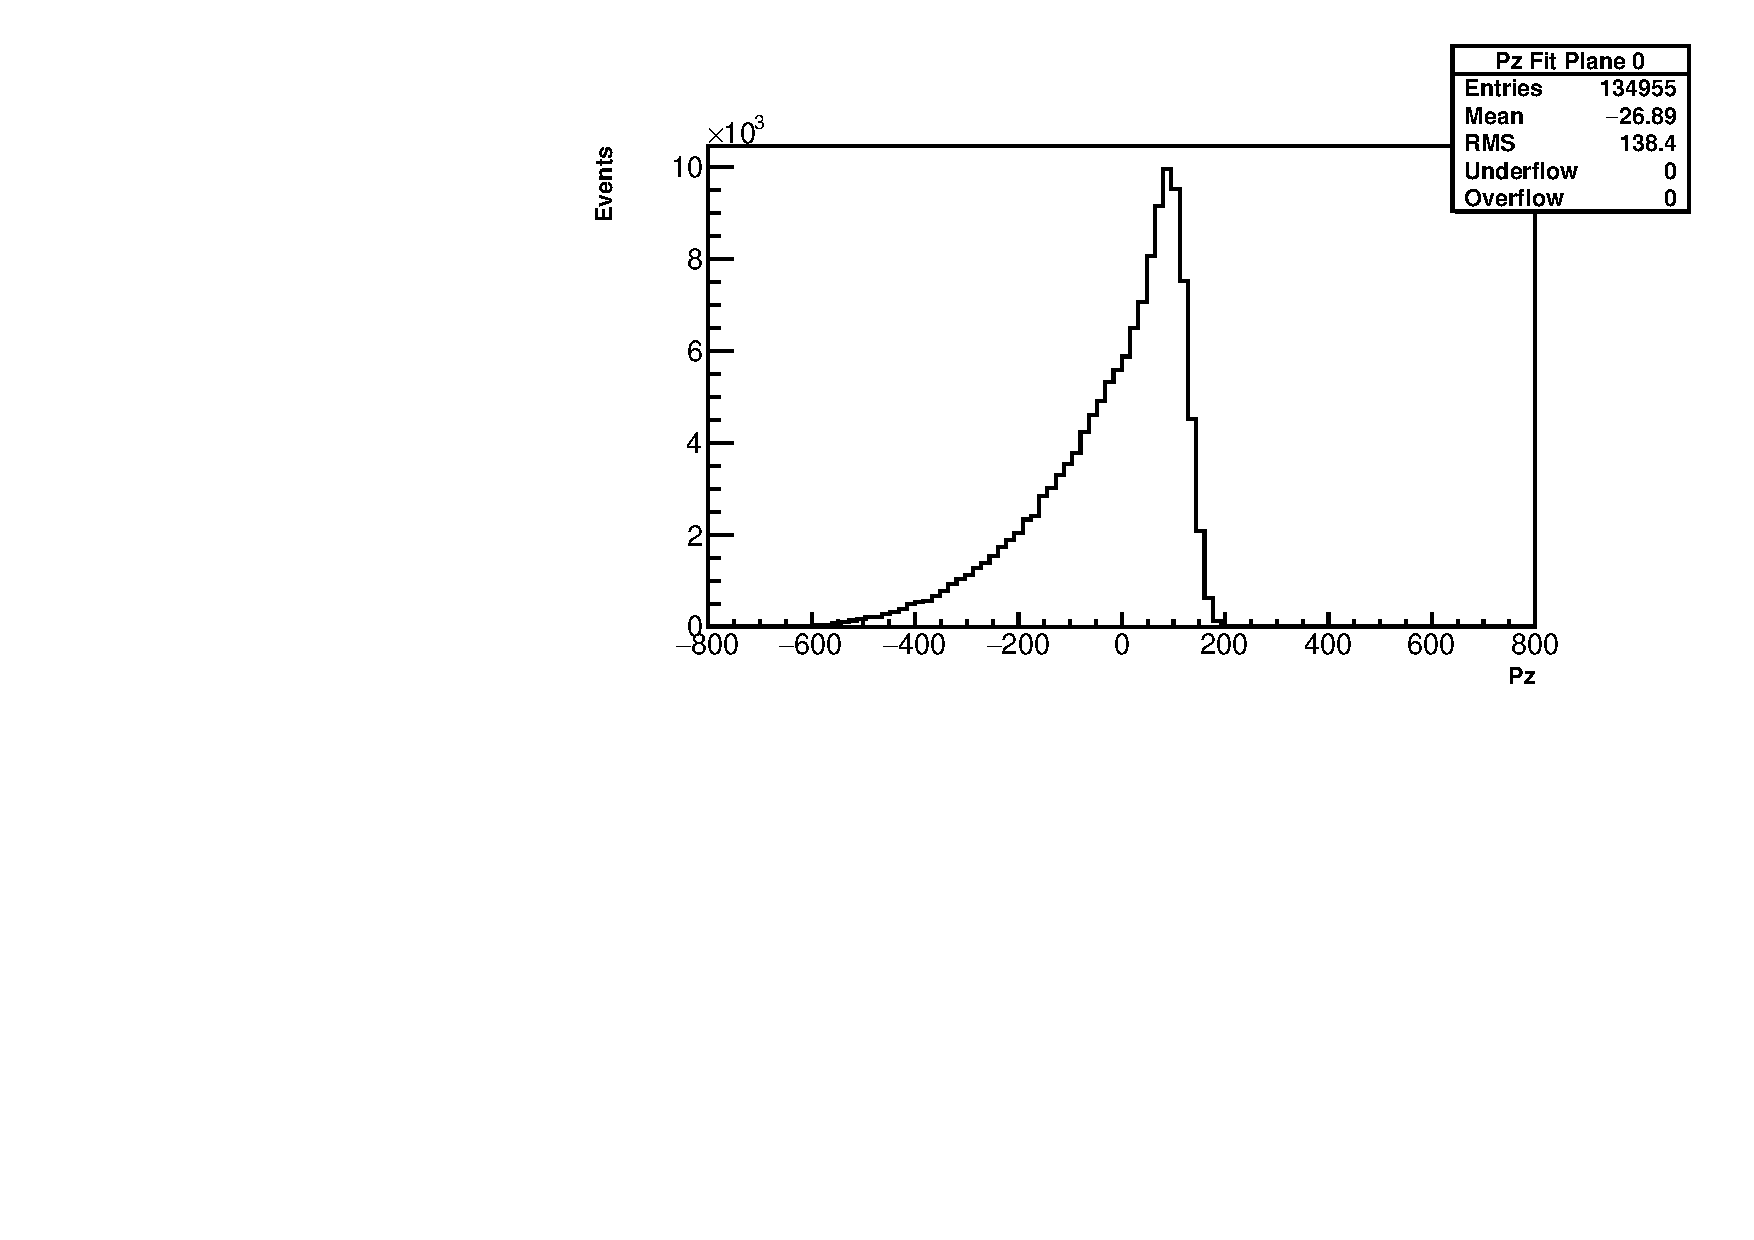
\includegraphics[width=1\textwidth]{Pzplane0} 
        \caption{Z momentum of the fit at plane 0. Some particles have outward radial momentum at the start of the fit (a negative value), and some inward, with all particles curving inward through the fit.}
    \end{subfigure}

    \caption{Momentum fit parameters on plane 0. Remember, the coordinate system is such that X is forward with the planes parallel, Y vertically up, and Z horizontal. The distributions here are very similar to truth as desired, which can be seen in the following truth residual plots.}
\end{figure}


\begin{figure}
    \centering
    \begin{subfigure}[]{0.55\textwidth}
        \centering
        \includegraphics[width=1\textwidth]{Xplane0} 
        \caption{X position from the fit at plane 0. Made up of individual delta functions since fits start at discrete 0 planes before each module. No tracks with the current Geane fitting starts at module 7 or 8 since such tracks don't hit enough planes to be fit.}
    \end{subfigure}

    \begin{subfigure}[]{0.55\textwidth}
        \centering
        \includegraphics[width=1\textwidth]{Yplane0} 
        \caption{Y position from the fit at plane 0. Bounded nicely by the measurement range of the detectors. The storage region width can be seen.}
    \end{subfigure}
    
    \begin{subfigure}[]{0.55\textwidth}
        \centering
        \includegraphics[width=1\textwidth]{Zplane0} 
        \caption{Z position of the fit at plane 0. There is an interesting spiky structure to the distribution, coming from how the detectors are staggered and shifted, and the incoming distribution of positrons. A larger negative value indicates a greater radial position. As a reminder this distribution is seen in truth as well.}
    \end{subfigure}

    \caption{Position fit parameters on plane 0. Remember, the coordinate system is such that X is forward with the planes parallel, Y vertically up, and Z horizontal. The distributions here are very similar to truth as desired, which can be seen in the following truth residual plots.}
\end{figure}


\begin{figure}
    \centering
    \begin{subfigure}[]{0.6\textwidth}
        \centering
        \includegraphics[width=1\textwidth]{P0TruthRes} 
        \caption{Momentum truth residual on plane 0. The distribution has an RMS of about 40 MeV.}
    \end{subfigure}

    \begin{subfigure}[]{0.6\textwidth}
        \centering
        \includegraphics[width=1\textwidth]{P0TruthResVsP} 
        \caption{Momentum truth residual on plane 0 vs P. As the momentum increase the spread in the residual increases, with the core staying relatively tight.}
    \end{subfigure}
    
    \begin{subfigure}[]{0.6\textwidth}
        \centering
        \includegraphics[width=1\textwidth]{Px0TruthRes} 
        \caption{X momentum truth residual on plane 0. Has an RMS of about 30 MeV. There are large tails in the distribution.}
    \end{subfigure}

    \caption{Momentum truth residuals on plane 0. Units are MeV. Most of the momentum and momentum spread is in the forward X direction. For real examination all of these plots should be split up according to the momentum of the track.}
\end{figure}


\begin{figure}
    \centering
    \begin{subfigure}[]{0.6\textwidth}
        \centering
        \includegraphics[width=1\textwidth]{P0TruthResRel} 
        \caption{Relative momentum truth residual on plane 0. There is about a 2\% resolution to the track fitting.}
    \end{subfigure}

    \begin{subfigure}[]{0.6\textwidth}
        \centering
        \includegraphics[width=1\textwidth]{P0TruthResVsPRel} 
        \caption{Relative momentum truth residual on plane 0 vs P. There is a tendency of the track fitting to overestimate the momentum of the track for some high momentum tracks.}
    \end{subfigure}
    
    \begin{subfigure}[]{0.6\textwidth}
        \centering
        \includegraphics[width=1\textwidth]{Px0TruthResRel} 
        \caption{X relative momentum truth residual on plane 0.}
    \end{subfigure}

    \caption{Relative momentum truth residuals on plane 0. For real examination all of these plots should be split up according to the momentum of the track.}
\end{figure}



\begin{figure}
    \centering
    \begin{subfigure}[]{0.6\textwidth}
        \centering
        \includegraphics[width=1\textwidth]{Py0TruthRes} 
        \caption{Y momentum truth residual on plane 0. The distribution has an RMS of about 4 MeV indicating the vertical momentum is pretty well measured, though tracks generally do not have much vertical momentum.}
    \end{subfigure}

    \begin{subfigure}[]{0.6\textwidth}
        \centering
        \includegraphics[width=1\textwidth]{Py0TruthResVsP} 
        \caption{Y momentum truth residual on plane 0 vs Py. There is a pretty tight core and some small corners in the distribution.}
    \end{subfigure}
    
    \begin{subfigure}[]{0.6\textwidth}
        \centering
        \includegraphics[width=1\textwidth]{Pz0TruthRes} 
        \caption{Z momentum truth residual on plane 0. Has an RMS of about 3 MeV, indicating the horizontal momentum is pretty well measured, though tracks generally do not have much horizontal momentum.}
    \end{subfigure}

    \caption{Momentum truth residuals on plane 0. Units are MeV. For real examination all of these plots should be split up according to the momentum of the track.}
\end{figure}

\clearpage

\begin{figure}
    \centering
    \begin{subfigure}[]{0.6\textwidth}
        \centering
        \includegraphics[width=1\textwidth]{X0TruthRes} 
        \caption{X position truth residual on plane 0. The distribution is a spike indicating that the X position of the fit is taken as known when fitting. Non-zero values indicate something is wrong with the fitting.}
    \end{subfigure}

    \begin{subfigure}[]{0.6\textwidth}
        \centering
        \includegraphics[width=1\textwidth]{Y0TruthRes} 
        \caption{Y position truth residual on plane 0. Has an RMS of about 740 $\mu$m as expected from simple geometry arguments coming from the 150 $\mu$m smearing. Even though particles do not curve much in Y, the straws don't measure the vertical position very well.}
    \end{subfigure}
    
    \begin{subfigure}[]{0.6\textwidth}
        \centering
        \includegraphics[width=1\textwidth]{Z0TruthRes} 
        \caption{Z position truth residual on plane 0. Has an RMS of about 135 $\mu$m as expected from simple geometry arguments coming from the 150 $\mu$m smearing. Better than the Y residual since both straws measure mostly in the horizontal direction, in spite of the fit having to deal with the curvature of the tracks.}
    \end{subfigure}

    \caption{Position truth residuals on plane 0. Units are mm. For real examination all of these plots should be split up according to the momentum of the track.}
\end{figure}







\end{document}
